% !TEX program = pdflatex
% !TEX encoding = UTF-8 Unicode

% Plantilla, basada en la clase `scrbook` del paquete KOMA-script,  para la elaboración de un TFG siguiendo las directrices del la comisión del Grado en Matemáticas de la Universidad de Granada.

% Francisco Torralbo Torralbo

\documentclass[print, color]{ugrTFG}

% Importamos paquetes
\setlength{\parskip}{5pt}%
%\setlength{\parskip}{\baselineskip}
\setlength{\parindent}{0pt}%
\DeclareMathOperator{\im}{Im}
\DeclareMathOperator{\id}{id}
\DeclareMathOperator{\interior}{Int}
\DeclareMathOperator{\sd}{sd}
\DeclareMathOperator{\bd}{Bd}
\DeclareMathOperator{\obj}{\textit{Obj}}
\DeclareMathOperator{\diam}{diam}
\DeclareMathOperator{\st}{st}
% VERSIÓN ELECTRÓNICA PARA TABLETA
% Cambiando la opción "print" por "tablet" generaremos un pdf adaptado para leerlo en tabletas de 9 pulgadas.

% -------------------------------------------------------------------
% INFORMACIÓN DEL TFG Y EL AUTOR
% -------------------------------------------------------------------

\newcommand{\miTitulo}{Aplicación de la topología algebraica en redes neuronales\xspace}
\newcommand{\miNombre}{Pablo Olivares Martínez\xspace}
\newcommand{\miGrado}{Grado en Ingeniería Informática y Matemáticas}
\newcommand{\miFacultad}{Facultad de Ciencias Escuela Técnica Superior de Ingenierías Informática y de Telecomunicación}
\newcommand{\miUniversidad}{Universidad de Granada}

% Añadir tantos tutores como sea necesario separando cada uno de ellos mediante el comando `\medskip` y una línea en blanco
\newcommand{\miTutor}{
  Miguel Ortega Titos \\ \emph{Departamento de Geometría y Topología} 

  % Añadir tantos tutores como sea necesario. 

  \medskip
  Julián Luengo Martín \\ \emph{Departamento de Ciencias de la Computación e Inteligencia Artificial}
}
\newcommand{\miCurso}{2023-2024\xspace}

\hypersetup{
	pdftitle={\miTitulo},
	pdfauthor={\textcopyright\ \miNombre, \miFacultad, \miUniversidad}
}

\begin{document}

\maketitle

% -------------------------------------------------------------------
% FRONTMATTER
% -------------------------------------------------------------------
\frontmatter % Desactiva la numeración de capítulos y usa numeración romana para las páginas

% !TeX root = ../tfg.tex
% !TeX encoding = utf8
%
%*******************************************************
% Declaración de originalidad
%*******************************************************

\thispagestyle{empty}

\hfill\vfill

\textsc{Declaración de originalidad}\\\bigskip

D./Dña. \miNombre \\\medskip

Declaro explícitamente que el trabajo presentado como Trabajo de Fin de Grado (TFG), correspondiente al curso académico \miCurso, es original, entendido esto en el sentido de que no he utilizado para la elaboración del trabajo fuentes sin citarlas debidamente.
\medskip

En Granada a \today 
\vspace{3cm}
\begin{center} 
	\begin{figure}[H]
		\center
		
\includegraphics[width=35mm]{img/firma.jpeg}
	\end{figure}
	
Fdo: \miNombre 

\end{center}

\vfill

\cleardoublepage
\endinput
   
% !TeX root = ../tfg.tex
% !TeX encoding = utf8

%*******************************************************
% Dedication
%*******************************************************
\thispagestyle{empty}
\phantomsection 
\pdfbookmark[1]{Dedicatoria}{Dedicatoria}

\hfill
\vfill

\begin{flushright}
\itshape
A mi familia y amigos, \\
y en especial a Inés.
\end{flushright}

\vfill

\cleardoublepage
\endinput
                % Opcional
% !TeX root = ../tfg.tex
% !TeX encoding = utf8

%*******************************************************
% Table of Contents
%*******************************************************
\phantomsection
\pdfbookmark[0]{\contentsname}{toc}

\setcounter{tocdepth}{2} % <-- 2 includes up to subsections in the ToC
\setcounter{secnumdepth}{3} % <-- 3 numbers up to subsubsections

\tableofcontents 

%*******************************************************
% List of Figures and of the Tables
%*******************************************************

    % *******************************************************
    %  List of Figures
    % *******************************************************    
    \phantomsection 
    % \listoffigures

    %*******************************************************
    % List of Tables
    %*******************************************************
    \phantomsection 
    % \listoftables
    
    %*******************************************************
    % List of Listings
    % The package \usepackage{listings} is needed
    %*******************************************************      
	  % \phantomsection 
    % \renewcommand{\lstlistlistingname}{Listados de código}
    % \lstlistoflistings 

\cleardoublepage
            
% !TeX root = ../tfg.tex
% !TeX encoding = utf8

%*******************************************************
% Agradecimientos
%*******************************************************

\chapter{Agradecimientos}

Quisiera comenzar agradeciendo a mis tutores, Miguel y Julián, por su gran ayuda
y dedicación en todo momento de este trabajo.
\bigskip

A mis padres y hermanos, así como a mis abuelos, por apoyarme de manera
incondicional desde la distancia y no dejar que me rindiera.
\bigskip

También quisiera agradecer a todos aquellos compañeros y amigos que, de una forma
u otra, me han ayudado con este trabajo tanto con sus ideas y opiniones como con
su aliento.
\bigskip

Por último, quisiera agradecérselo a Inés. Por tu paciencia y tu apoyo continuo,
por estar a mi lado cuando más lo necesitaba, gracias.

\cleardoublepage
\endinput            % Opcional

% !TeX root = ../tfg.tex
% !TeX encoding = utf8
%
%*******************************************************
% Summary
%*******************************************************

\selectlanguage{english}
\chapter{Abstract}

This Bachelor's Thesis explores the integration of Topological Data Analysis (TDA)
with convolutional neural networks (CNNs) to clarify and enhance our
understanding of how CNNs manipulate data. Given the common perception of CNNs as
\enquote{black boxes} due to the opacity on their internal decision-making
processes, this work adopts an alternative approach through the application of persistent
homology techniques, a key tool in TDA. This allows for a detailed analysis of the
data structure during CNN processing, facilitating greater transparency and
understanding of these networks' internal workings from a topological point of view.

The study focuses on the applicability of persistent homology to provide an additional
layer of explainability and optimization to deep learning models. The underlying
theory is explored, and implementations are carried out in practical cases using
advanced network architectures such as ResNet, EfficientNet and DenseNet. Through
controlled experiments, it is demonstrated that topological regulation not only
improves the performance of CNNs in image classification and transfer learning
tasks, but also offers new insights into the data structure throughout the learning
process.

Specific results indicate that different configurations in CNN models significantly
influence the topological characteristics of the data. The dynamics of the
architectures studied show an initial tendency to simplify the data, possibly to
remove noise and irrelevant details. However, as learning progresses, the
topological complexity of the data increases, suggesting a deliberate strategy to
develop richer and more detailed representations, thereby facilitating better
differentiation between classes.

The implementation of a topological regularizer in selected models such as
EfficientNet-B0 and DenseNet-121 has proven to be particularly promising. This approach
adjusts the topological complexity of the data in a way that reflects a significant
improvement in the accuracy and efficacy of classification. Moreover, it is observed
that knowledge transfer markedly improves when the data topology is appropriately
manipulated, suggesting that topological modifications could be an effective
strategy for optimizing CNNs.

In conclusion, this document not only enhances the understanding of CNNs'
internal mechanisms through TDA but also marks a step towards more transparent
and reliable artificial intelligence (AI) models. The findings shows the utility
of TDA in the field of deep learning, proposing a new alternatives for
explainability and efficiency that may be interesting to consider in the future
evolution of computer vision and data science.

\bigskip
\textbf{Keywords}: convolutional neural networks, topological data analysis,
persistent homology, AI explainability, optimization of deep learning models, transfer
learning.

% Al finalizar el resumen en inglés, volvemos a seleccionar el idioma español para el documento
\selectlanguage{spanish}
\chapter{Resumen}

Este Trabajo de Fin de Grado (TFG) explora la integración del Análisis de Datos
Topológico (TDA) con redes neuronales convolucionales (CNNs) para clarificar y
mejorar nuestra comprensión de cómo las CNNs manipulan los datos. Dada la percepción
común de las CNNs como \enquote{cajas negras} debido a la opacidad en sus
procesos de toma de decisiones internos, este trabajo adopta un enfoque alternativo
mediante la aplicación de técnicas de homología persistente, una herramienta
clave en TDA. Esto permite un análisis detallado de la estructura de datos durante
el procesamiento en las CNNs, facilitando una mayor transparencia y
entendimiento de los mecanismos internos de estas redes desde un punto de vista
topológico.

El estudio se centra en la aplicabilidad de la homología persistente para
proporcionar una mayor explicabilidad y optimización de los modelos de
aprendizaje profundo. Se explora la teoría matemática subyacente, para
posteriormente realizar implementaciones en casos prácticos utilizando
arquitecturas de CNNs avanzadas como ResNet, EfficientNet y DenseNet. A través
de experimentos controlados, se demuestra que la regulación topológica no solo mejora
el rendimiento de las CNNs en tareas de clasificación de imágenes y de transferencia
de conocimiento, sino que también ofrece nuevas perspectivas sobre la estructura
de los datos a lo largo del proceso de aprendizaje.

Los resultados indican que las diferentes configuraciones en los modelos de CNNs
influyen significativamente en las características topológicas de los datos. La dinámica
de las arquitecturas estudiadas muestra una tendencia inicial a simplificar los datos,
posiblemente para eliminar ruido y detalles irrelevantes. Sin embargo, a medida
que avanza el aprendizaje, la complejidad topológica de los datos aumenta,
sugiriendo una estrategia deliberada para obtener representaciones más ricas y
detalladas, facilitando así una mejor diferenciación entre clases.

La implementación de un regularizador topológico en modelos como EfficientNet-B0
y DenseNet-121 ha demostrado ser particularmente prometedora. Este enfoque
ajusta la complejidad topológica de los datos de manera que refleja una mejora
significativa en la precisión y eficacia de la clasificación. Además, se observa
que la transferencia de conocimiento mejora considerablemente cuando la
topología de los datos se manipula adecuadamente, sugiriendo que las modificaciones
topológicas podrían ser una estrategia efectiva para optimizar las CNNs.

En conclusión, este documento no solo mejora la comprensión de los mecanismos
internos de las CNNs a través de TDA, sino que también marca un paso hacia modelos
de inteligencia artificial (IA) más transparentes y confiables. Los hallazgos
destacan la utilidad del TDA en el campo del aprendizaje profundo, proponiendo nuevas
alternativas para la explicabilidad y eficiencia que pueden ser interesantes de considerar
en la evolución futura de la visión artificial y la ciencia de datos.

\bigskip
\textbf{Palabras clave}: redes neuronales convolucionales, análisis de datos
topológico, homología persistente, explicabilidad en IA, optimización de modelos
de aprendizaje profundo, transferencia de conocimiento.

\endinput                    
% !TeX root = ../tfg.tex
% !TeX encoding = utf8
%
%*******************************************************
% Introducción
%*******************************************************

% \manualmark
% \markboth{\textsc{Introducción}}{\textsc{Introducción}}

\chapter{Introducción}

\section{Contexto}

El desarrollo humano ha sido constantemente impulsado por avances tecnológicos que
han redefinido nuestra comprensión e interacción con mundo. Desde la invención
de la imprenta hasta la revolución digital actual, cada era ha estado marcada por
innovaciones clave. En particular, la invención de los ordenadores y el avance de
las tecnologías de la información han convergido en la capacidad de generar,
almacenar y analizar grandes volúmenes de datos. Este volumen de información ha desencadenado
lo que ahora conocemos como la Era de la Información, que se caracteriza por el
desarrollo de algoritmos avanzados que extraen valor de estos datos de manera
automática y eficiente.

Dentro de esta revolución tecnológica, el aprendizaje profundo y, en particular,
las redes neuronales convolucionales (CNNs) \cite{bengio2017deep} han emergido como
útiles herramientas, especialmente en el ámbito de la visión artificial. Estos modelos
son capaces de identificar patrones complejos en datos visuales, superando a
menudo el rendimiento humano en tareas de reconocimiento de imágenes. Sin embargo,
las decisiones tomadas por las CNN a menudo son opacas y difíciles de
interpretar, lo que ha llevado a que se les describa como \enquote{cajas negras}.

Ante este problema, han surgido diversas técnicas para clarificar cómo estas redes
toman decisiones. Una de las más novedosas y prometedoras es el análisis de
datos topológico (TDA) \cite{dey2022computational}, que emplea herramientas de la
topología algebraica para ofrecer soluciones. El TDA busca comprender la
\enquote{forma} de los datos, ofreciendo así conocimiento sobre cómo las CNNs
estructuran y manipulan la información a nivel global, no solo basándose en instancias
individuales.

En este trabajo, aplicaremos técnicas de TDA para desentrañar cómo las CNNs
procesan y transforman conjuntos de datos, con el objetivo de comprender los mecanismos
subyacentes de estos modelos de aprendizaje profundo y así proporcionar nuevas claves
que nos permitan aprovecharlas mejor. Al enfocarnos en las estructuras globales
de los datos en lugar de cambios individuales, esperamos ofrecer una comprensión
más clara y detallada de cómo trabajan estas redes, contribuyendo así a una
mayor comprensión y confianza en los algoritmos de aprendizaje profundo.

El TDA es un campo relativamente reciente. A comienzo de los años 90, bajo la
premisa de que los datos tienen una \enquote{forma}, matemáticos como Patrizio
Frosini o Vanessa Robins estudiaron las propiedades que podían extraerse en el
estudio de la distancia entre variedades \cite{Frosini_1990} y estructuras
relacionadas por el homomorfismo de inclusión \cite{robins1999towards}. Estas ideas
cautivaron a Edelsbrunner, quien les dio forma en lo que hoy se conoce como
homología persistente, junto con un algoritmo para calcularla y visualizarla de manera
efectiva \cite{edelsbrunner2002topological}. La homología persistente es
actualmente la piedra angular del TDA, permitiendo el análisis de características
topológicas que persisten a través de diferentes escalas. La homología
persistente resuelve desafíos en la selección de parámetros al codificar
información de todos los valores posibles. En 2008, Gunnar Carlsson
\cite{carlsson2009topology} dio un paso adelante al reformular la homología
persistente dentro del ámbito del álgebra conmutativa, proporcionando lo que hoy
conocemos como código de barras, facilitando su comprensión y ampliando su
aplicabilidad en ciencia de datos y otras áreas tecnológicas. Desde entonces,
varios autores como Liwen Zhang, Gregory Naitzat y Lek-Heng Lim \cite{naitzat2020topology}
han aplicado estas técnicas con el fin de comprender mejor el funcionamiento de las
CNN. Su trabajo mostraba que, efectivamente, las CNNs simplificaban la \enquote{forma}
de los datos. Inspirado por los resultados, German Magai \cite{magai2023deep} profundizó
en estos hallazgos para confirmar dichas afirmaciones.

\section{Motivación}

La comprensión del funcionamiento de los modelos de aprendizaje profundo ha
emergido como una necesidad en el campo de la ciencia de datos. Las CNNs, aunque
pesar de ser muy efectivas en muchas tareas de visión artificial, a menudo actúan
como \enquote{cajas negras}. Esto puede ser un problema, ya que nos impide
comprender por qué un modelo ha tomado ciertas decisiones que pueden ser
erróneas y por tanto ser incapaces de ofrecer solución al problema.

La topología es la rama de las matemáticas que estudia las transformaciones
continuas, por lo que nos ofrece una perspectiva única para investigar cómo las CNNs
procesan los datos. Aunque la topología es un área bastante abstracta de las
matemáticas, su uso en el análisis de datos complejos es relativamente nuevo y prometedor.
Dentro de este campo, la homología persistente aplicada en el marco del TDA se presenta
como una herramienta innovadora para descifrar la manera en que las CNNs modifican
la \enquote{forma} de los datos durante su procesamiento.

La aplicación de métodos topológicos a los problemas del aprendizaje profundo no
es solo novedosa, sino que también tiene un gran potencial para transformar nuestra
comprensión de los modelos complejos. Al explorar cómo el TDA puede mejorar la
transparencia y eficacia de las CNNs, este estudio no solo busca aclarar el funcionamiento
interno de estos modelos, sino que también se adentra en un campo poco explorado
que cruza varias disciplinas con el objetivo final de abrir nuevas vías de
investigación y aplicaciones prácticas no solo para mejorar la manera en que
interactuamos con estas tecnologías, sino también para entender y confiar en las
decisiones que toman.

\section{Estructura del trabajo}

Con el fin de profundizar en la comprensión de los modelos de CNNs desde la
perspectiva de la homología persistente, este trabajo se ha estructurado en cuatro
partes.

La primera parte se centra en establecer las bases teóricas de la homología persistente,
para lo cual se explora detalladamente la teoría de la homología simplicial. Esta
área de la topología algebraica se desarrolló originalmente para estudiar el concepto
de \enquote{agujero} en diversas dimensiones mediante el uso de símplices, que son
estructuras que generalizan el concepto de triángulo a múltiples dimensiones.
Los símplices suelen agruparse en lo que se conoce como complejos simpliciales, que
son conjuntos de símplices que se combinan de manera que sus intersecciones cumplen
ciertas propiedades. Estas estructuras forman parte de una familia más general, conocida
como CW-complejos, que ofrecen un marco más flexible para la construcción de
espacios topológicos a través de la unión de piezas llamadas celdas. También exploraremos
la sucesión de Mayer-Vietoris, una herramienta poderosa en topología algebraica
que permite descomponer espacios topológicos complejos en uniones de subespacios
más simples, facilitando el cálculo de sus invariantes topológicos como los módulos
de homología y la relación de estos con conceptos como la conexión. Con todo
esto podemos finalmente introducir la homología persistente y el Teorema de
Correspondencia, el cual nos dará las herramientas necesarias que hoy emplea el TDA.

En la segunda parte de este trabajo, se realizará un estudio detallado sobre los
principios del aprendizaje profundo que fundamentan las CNNs, comenzando con un repaso
histórico desde las neuronas artificiales básicas hasta los modelos de CNN más avanzados
en la actualidad. Esta sección abordará tanto las propiedades fundamentales de
las CNNs como sus características específicas, mostrando cómo estas han evolucionado
para proporcionar mejores y más eficientes predicciones en el ámbito de la clasificación
de imágenes.

Finalmente introduciremos el TDA, explicando sus principios y técnicas, y exploraremos
su aplicación en el ámbito de las CNNs para comprender cómo la estructura de los
datos afecta el aprendizaje de la red. Esta exploración teórica establecerá la
base para los estudios y experimentos realizados en este trabajo. se expondrán los
resultados y la metodología empleada en un exhaustivo estudio de la homología persistente
y de las propuestas realizadas.

Para terminar, se presentan las conclusiones obtenidas y propuestas futuras para
el estudio de la manera en que las CNNs cambian la \enquote{forma} de los datos.

\section{Objetivos}

El presente trabajo propone una serie de objetivos con el fin de profundizar en
las bases de la homología persistente y realizar un estudio práctico en el
ámbito de las CNNs:

\begin{enumerate}
	\item En el ámbito de las \textbf{matemáticas} se propuso como objetivo
	principal profundizar en los contenidos de la topología algebraica y una
	introducción rigurosa a la homología persistente. Con dicho fin, la
	\autoref{part:math} cumple con los siguientes puntos:
	\begin{itemize}
		\item Se realiza una descripción de las principales herramientas algebraicas
		necesarias para el estudio de la homología simplicial y la homología persistente
		\autoref{chapter:alg-fundamentals}.
		
		\item Se estudian los complejos simpliciales, objetos de estudio de la
		homología simplicial. Además, se exploran otras estructuras topológicas
		relevantes como los CW-complejos y las variedades topológicas en el
		\autoref{chapter:complex}.
		
		\item Se introduce la homología simplicial y una de sus principales herramientas,
		la sucesión de Mayer-Vietoris, además de su relación con la conexión topológica
		en el \autoref{chapter:homology}.
		
		\item Se introduce el concepto de homología persistente y su principal resultado,
		el Teorema de correspondencia, descritos en el \autoref{chapter:persistent-homology}.
	\end{itemize}
	
	\item Posteriormente, desde el ámbito del \textbf{aprendizaje profundo} se plantea
	comprender los principales modelos de CNNs en el ámbito de la clasificación de
	imágenes. Para ello, la \autoref{part:deep-learning} explora los siguientes conceptos:
	\begin{itemize}
		\item Se repasan los principales conceptos de inteligencia artificial,
		aprendizaje automático y visión artificial en el
		\autoref{chapter:concepts}.
		
		\item Se realiza un repaso histórico y del estado del arte de las CNNs en los
		Capítulos \ref{chapter:ann} y \ref{chapter:cnn}.
	\end{itemize}
	
	\item Finalmente, se propone realizar un estudio de las CNNs mediante el uso
	de técnicas de TDA y formalizar una propuesta en base a las conclusiones
	obtenidas. Para cumplir con estos objetivos, se han superados los siguientes
	hitos en la \autoref{part:proposal}:
	\begin{itemize}
		\item Se analiza cómo transforman diferentes modelos y elementos de las CNNs
		la homología persistente de los datos en el \autoref{chapter:analisis}.
		
		\item Se propone un regularizador topológico con el objetivo de mejorar la
		tasa de clasificación y la transferibilidad de los modelos en los Capítulos
		\ref{chapter:tda} y \ref{chapter:analisis}.
	\end{itemize}
\end{enumerate}

\section{Presupuesto}

La primera consideración en el coste de la elaboración del estudio viene dada
por la mano de obra empleada. El equipo empleado por el trabajador se trata de un
ordenador portátil valorado en 600€ y una vida útil de 6 años. El proyecto se ha
realizado durante un periodo de 10 meses y medio, donde en promedio se le ha dedicado
4 horas diarias en los días de semana, lo que se traduce en 20 horas semanales. Por
otro lado, según el portal de transparencia empresarial Glassdoor\footnote{\href{https://www.glassdoor.es/Sueldos/data-scientist-sueldo-SRCH_KO0,14.htm}{https://www.glassdoor.es/Sueldos/data-scientist-sueldo-SRCH\_KO0,14.htm}},
el salario de un científico de datos promedio en España se comprende en el rango
de los 30.000€ a 45.000€. Dado que el perfil del empleado es de junior,
supondremos un salario de 30.000€ anuales, lo que implica un salario de 15€ por
hora.

El coste derivado del entrenamiento de modelos de aprendizaje profundo suele ser
elevado debido al consumo energético de las GPUs y el tiempo de entrenamiento
necesario. Además, ha de tenerse en cuenta gastos derivados como mantenimiento y
refrigeración. Dado que se han entrenado un total de 88 modelos con tiempos de entrenamiento
medios de una hora, más algunas pruebas y expermientos, llegamos a la conclusión
que el tiempo total de GPU empleado es de unas 100 horas. En particular, se han empleado
dos Quadro RTX 8000, con un consumo de 260W por hora. Sabiendo que el precio de la
luz en Granada ronda los 0,1€/kWh en promedio, nos queda el presupuesto total
que figura en la \autoref{tab:presupuesto}.

\begin{table}[h!]
	\centering
	\begin{tabular}{|l|r|}
		\hline
		\textbf{Categoría}                     & \textbf{Costo}      \\
		\hline
		Mano de obra                           & 13,640€             \\
		\hline
		Amortización del equipo                & 87,50€              \\
		\hline
		Coste de energía (GPU)                 & 26€                 \\
		\hline
		Coste de mantenimiento y refrigeración & 20€                 \\
		\hline
		\textbf{Total}                         & \textbf{13,773,50€} \\
		\hline
	\end{tabular}
	\caption{Presupuesto detallado del estudio.}
	\label{tab:presupuesto}
\end{table}

\section{Planificación}

La organización de este trabajo supuso un reto desde comienzos del curso 2023-2024.
El hecho de tener que compaginar un curso completo con un trabajo de tal calibre
requería de una organización minuciosa. Por ello, desde comienzos de septiembre
de 2023 se comenzó a investigar y profundizar en los conceptos teóricos
requeridos para tener una comprensión profunda de la homología persistente. Esta
fase requirió de más tiempo del esperado, tal y como puede observarse en la
\autoref{fig:plan}. La principal complicación surgió debido a la aparición de requisitos
no contemplados en demostraciones puntuales que, junto a los exámenes, retrasó la
finalización del marco teórico matemático.

La etapa final del desarrollo teórico se compaginó con reuniones con los tutores
para ir concretando el camino de los experimentos y el planteamiento de hipótesis.
Esto llevó a que la implementación del código necesario se realizara en su
mayoría durante los meses de abril y mayo, que posteriormente iría siendo modificado
en función de las necesidades de la investigación y los resultados obtenidos.

\begin{figure}[H]
	\centering
	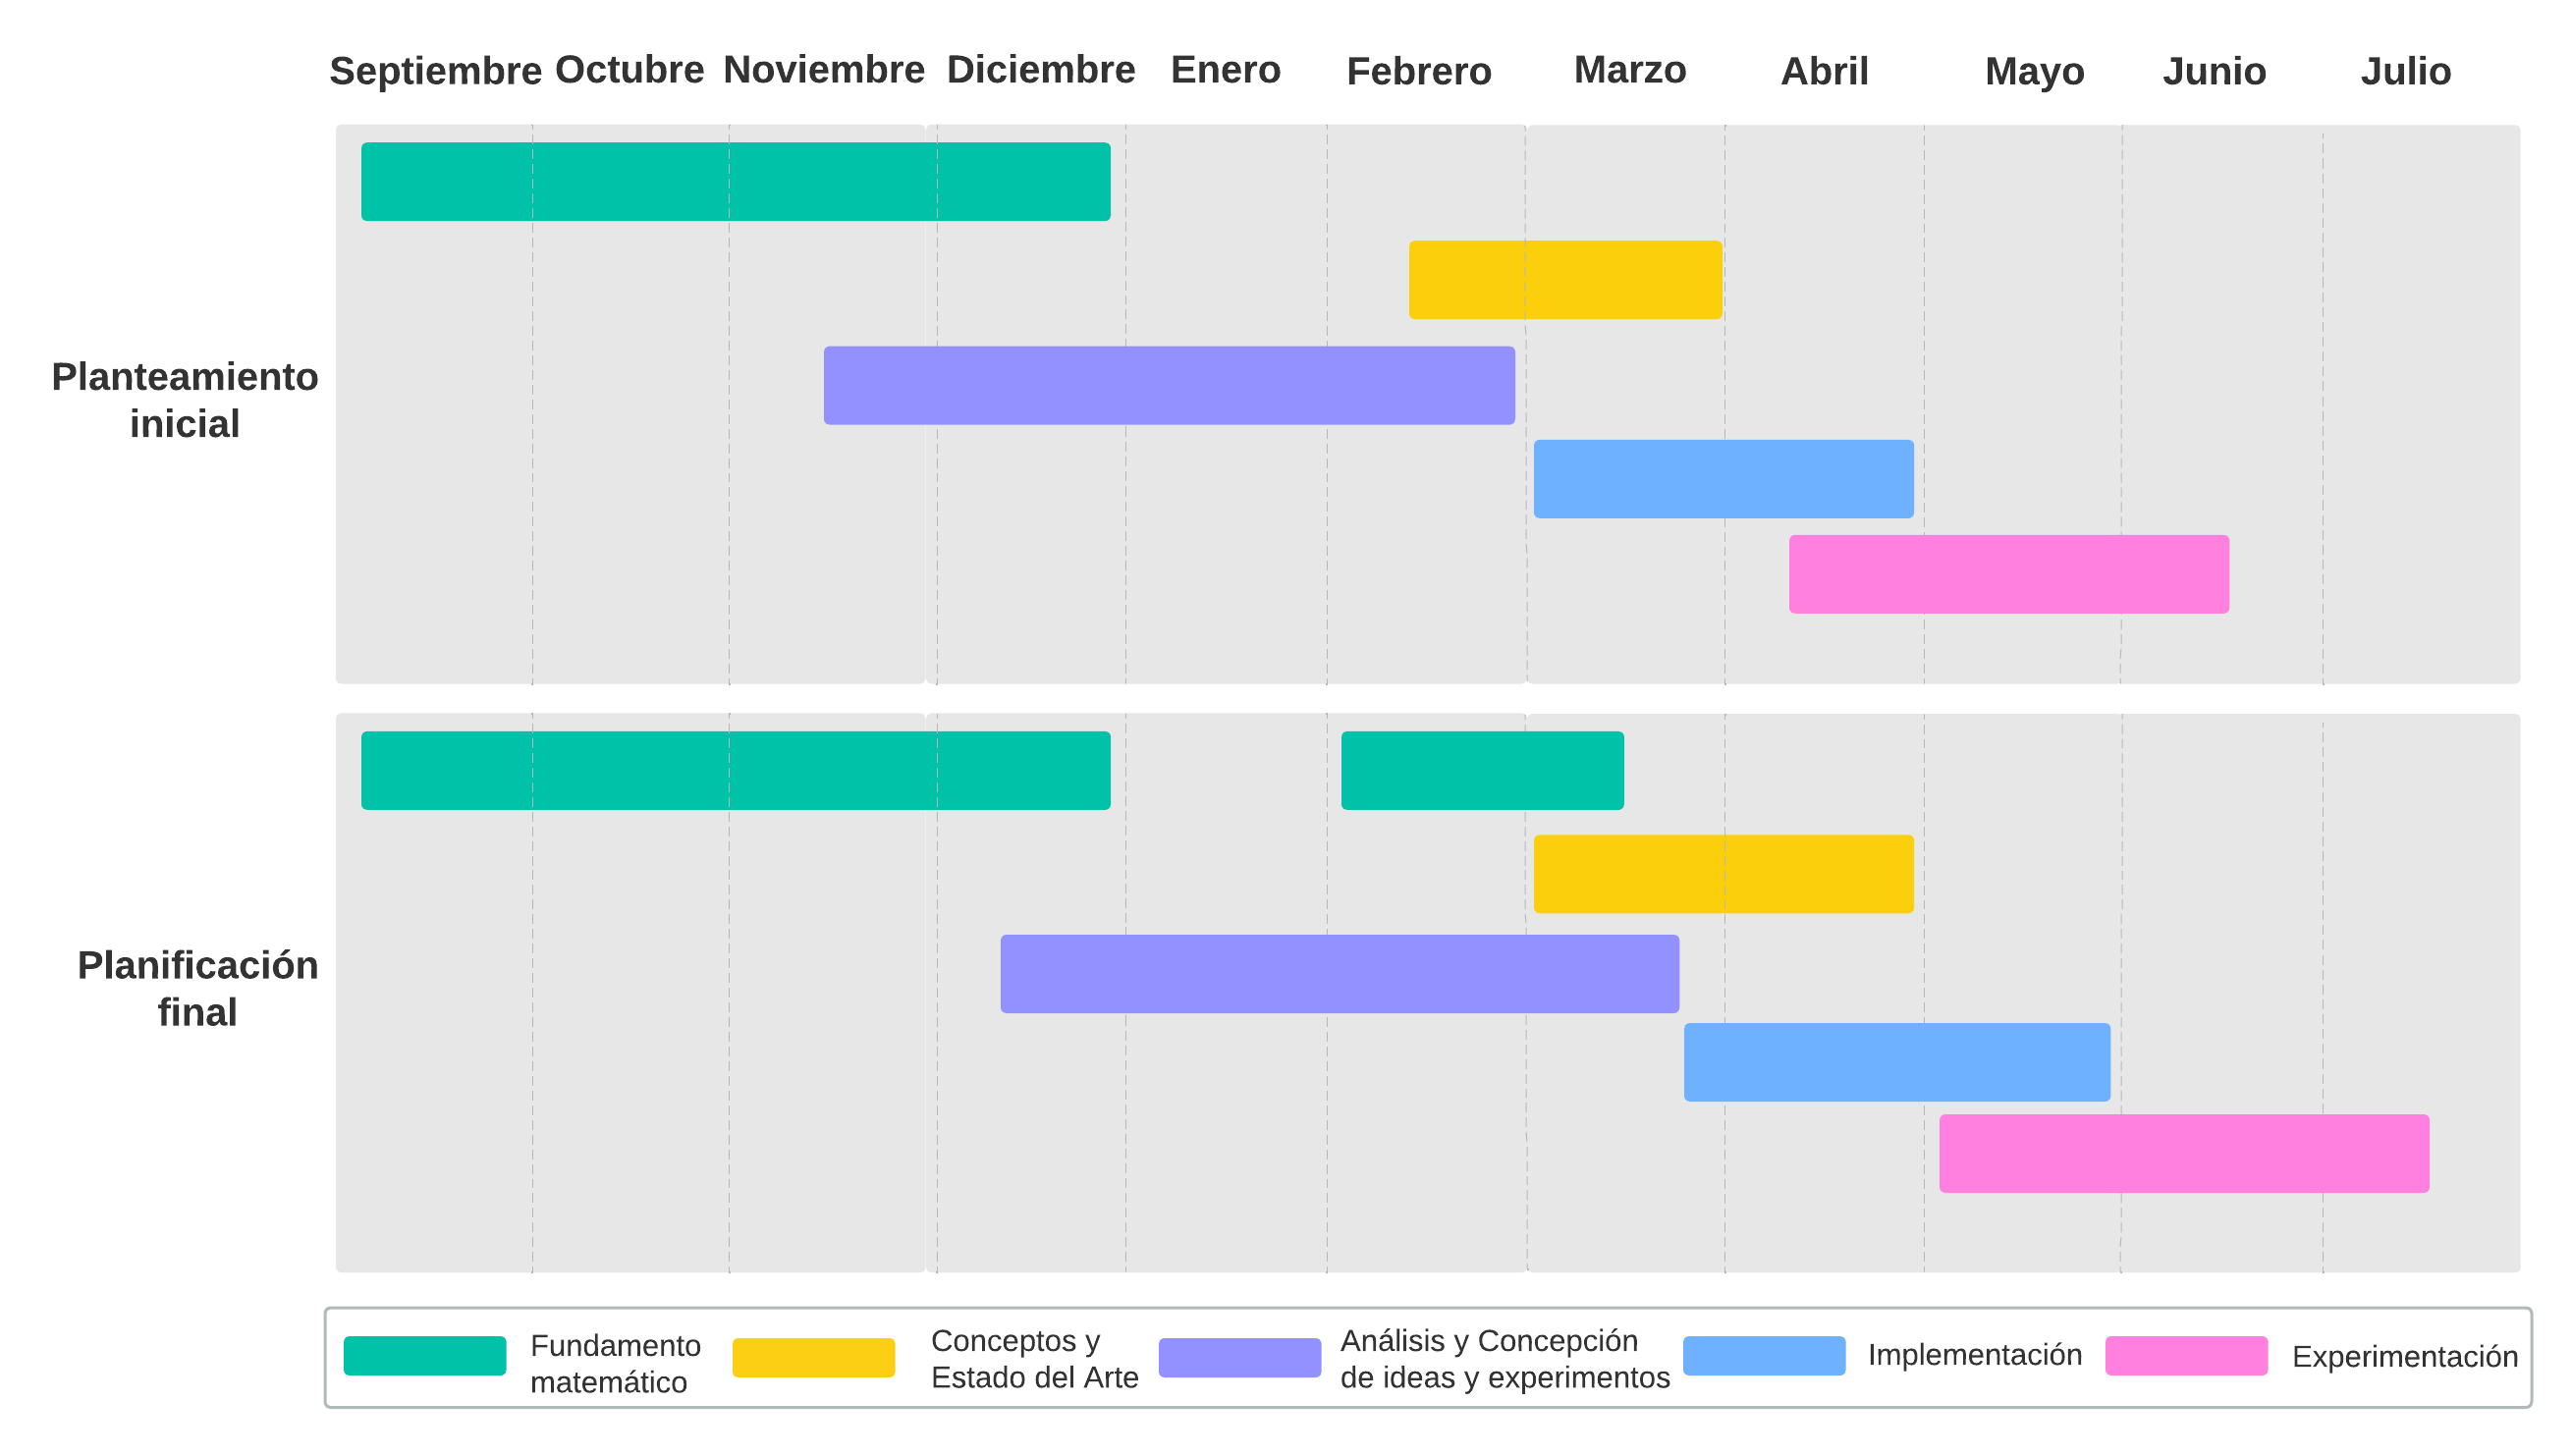
\includegraphics[width=150mm]{img/planificacion.png}
	\caption{Planificación temporal prepuesta frente a la finalmente realizada.}
	\label{fig:plan}
\end{figure}

\endinput               

% -------------------------------------------------------------------
% MAINMATTER
% -------------------------------------------------------------------
\mainmatter % activa la numeración de capítulos, resetea la numeración de las páginas y usa números arábigos

\part{Fundamento teórico} % Dividir un TFG en partes OPCIONAL
% Añadir tantos capítulos como sea necesario
% !TeX root = ../tfg.tex
% !TeX encoding = utf8

\chapter{Preliminares algebraicos}

\section{Módulos}

\begin{definicion}
	Sea $R$ un anillo cuyo elemento identidad $1 \neq 0$. Un \textbf{$R$-módulo izquierdo} $A$ es un grupo abeliano aditivo junto con una función $p: R \times A \rightarrow A$ con $(r, a) \to ra$ tal que dados $r,r' \in R$, $a,a' \in A$ se tiene
	\begin{enumerate}
		\item $(r+r')+a = ra + r'a$
		\item $(rr')a = r(r'a)$
		\item $r(a+a') = ra + ra'$
		\item $1a = a$
	\end{enumerate}
\end{definicion}

De la definición anterior se sigue que $0a = 0$ y $(-1)a = -a$.

De manera análoga, definimos \textbf{$R$-módulo derecho} donde el anillo actúa por la izquierda en vez de por la derecha de forma que $p: A \times R \rightarrow A$. Si $R$ es un anillo conmutativo, los $R$-módulos izquierdos y derechos coinciden y les llamamos simplemente $R$-módulos. Como los resultados de $R$-módulos izquierdos y derechos son análogos, trabajaremos simplemente con los $R$-módulos izquierdos y nos referiremos a ellos como $R$-módulos a menos que se indique explícitamente lo contrario.

\begin{ejemplo}
	ej
\end{ejemplo}

\begin{definicion}
	Sea $A$ un $R$-módulo izquierdo y $S$ un subconjunto de $A$. Diremos que $S$ es un submódulo izquierdo de $A$, esto es, $S \subset A$, si $S$ es cerrado respecto a la suma y si $r,s \in S$ entonces $rs \in S$. Por tanto, $S$ es un $R$-módulo.
\end{definicion}

Si un submódulo de $R$ es un subconjunto $L \subset R$ cerrado respecto a la suma tal que $rL \subset L$ para todo $r \in R$, lo llamaremos \textbf{ideal izquierdo} de $R$. Tomando un ideal izquierdo $L$ de $R$ y $A$ un $R$-módulo izquierdo, definimos el producto del ideal $L$ por el módulo $A$
\[ LA = \{\text{todas las sumas finitas } \sum l_ia_i, \text{ para } l_i \in L,\ a_i \in A \} \]
donde $LA$ es un submódulo de $A$. En particular, el producto de dos ideales izquierdos $LL'$ es también un ideal izquierdo y $(LL')A = L(L'A)$.

\begin{definicion}
	Sean $A$, $B$ $R$-módulos. Definimos el \textbf{homomorfismo de $R$-módulos} de $A$ a $B$ como la aplicación $\alpha: A \rightarrow B$ tal que
	\begin{enumerate}
		\item $\alpha(a+a') = \alpha a + \alpha a'$
		\item $\alpha(ra) = r(\alpha a)$
	\end{enumerate}
	para todo $a,a' \in A$, $r \in R$.
\end{definicion}

También es frecuente escribir el homomorfismo de $R$-módulos $\alpha: A \rightarrow B$ como $A \xrightarrow{\alpha} B$.

Cuando $\alpha: A \rightarrow B$ sea un homomorfismo de $R$-módulos, diremos que $A$ es el \textbf{dominio} y $B$ el \textbf{rango}. La \textbf{imagen} de $\alpha$ es el conjunto $\im(\alpha) = \{ \alpha(a) : a \in A \}$. El \textbf{núcleo} será el conjunto de elementos que se anulan en su imagen, esto es, $\ker(\alpha) = \{ a \in A : \alpha(a) = 0 \}$. Diremos que $\alpha$ es un \textbf{epimorfismo} cuando $\alpha(A) = B$, un \textbf{monomorfismo} cuando $\ker(\alpha) = \{0\}$ y un \textbf{isomorfismo} si $\alpha$ es un epimorfismo y un monomorfismo a la vez. Si existe un isomorfismo entre $A$ y $B$ diremos que son \textbf{isomorfos} y lo notaremos $A \cong B$. Un homomorfismo $\omega: A \rightarrow A$ lo llamaremos \textbf{endomorfismo}.

Dados dos homomorfismos de $R$-módulos $\alpha_1, \alpha_2 : A \rightarrow B$, su \textbf{suma} $\alpha_1 + \alpha_2$ la definimos como $(\alpha_1 + \alpha_2)(a) = \alpha_1(a) + \alpha_2(a)$ para todo $a \in A$. Además, dados dos homomorfismos de $R$-módulos $\alpha: A \rightarrow B$, $\beta: B \rightarrow C$, su \textbf{composición} $\beta \circ \alpha: A \rightarrow C$ es también un homomorfismo de $R$-módulos. Nótese que para que la composición sea posible, el rango de $\alpha$ tiene que ser igual al dominio de $\beta$. En ocasiones usaremos la notación $\alpha\beta = \alpha \circ \beta$. Llamaremos \textbf{inversa} (por ambos lados) de $\alpha : A \rightarrow B$ al homomorfismo $\alpha^{-1} : B \rightarrow A$ tal que $\alpha^{-1} \circ \alpha = 1_A$ y $\alpha \circ \alpha^{-1} = 1_B$. Una \textbf{inversa izquierda} de $\alpha$ es una función $\gamma: A \rightarrow A$ tal que $\gamma \circ \alpha = 1_A$. No tiene por qué existir ni ser única.

\begin{definicion}
	Sea $\{A_i, \alpha_i\}$ una familia de $R$-módulos $A_i$ y homomorfismos entre ellos tal que $\alpha_i: A_i \rightarrow A_{i+1}$. Diremos que la secuencia
	\[ \cdots \xrightarrow{\alpha_{i-2}} A_{i-1} \xrightarrow{\alpha_{i-1}} A_i \xrightarrow{\alpha_{i}} A_{i+1} \xrightarrow{\alpha_{i+1}} \cdots \]
	es \textbf{exacta} cuando $\im \alpha_i = \ker \alpha_{i+1}$.
\end{definicion}

Para cada submódulo $T \subset B$, la inclusión de $T$ en $B$ es un monomorfismo $i: T \rightarrow B$. Las \textbf{clases laterales} de $T$ en $B$ son los conjuntos $b + T = \{b + t : t \in T\}$ donde $b \in B$. Dos clases laterales $b_1 + T$, $b_2 + T$ son iguales si $b_1 - b_2 \in T$. Como $T$ es un submódulo, el grupo abeliano $B/T$ se convierte en un $R$-módulo cuando $r(b+T) = rb + T$ para todo $r \in R$. A este $R$-módulo lo llamaremos el \textbf{módulo cociente} de $B$ sobre $T$. El homomorfismo $\pi: B \rightarrow B/T$ tal que $\pi(b) = b + T$ es un epimorfismo que llamaremos \textbf{proyección canónica} de $B$.

\begin{proposicion}\label{prop:first_iso}

Sea \( \beta: B \rightarrow B' \) un homomorfismo de módulos con \( T \subset \ker \beta \). Existe entonces un único homomorfismo de módulos \( \beta': B/T \rightarrow B' \) con \( \beta'\pi = \beta \); es decir, el siguiente diagrama con \( \beta(T) = 0 \)
\[
\begin{array}{ccc}
	B & \stackrel{\pi}{\longrightarrow} & B/T \\
	& \searrow \beta & \downarrow \beta' \\
	& & B'
\end{array}
\]
es conmutativo.
\end{proposicion}

\begin{proof}
Definamos \( \beta'(b + T) = \beta(b) \). Por estar $T$ contenida en el núcleo de $\beta$, la función está bien definida. En efecto, si $a,b \in B$ entonces $a+T = b+T \Rightarrow a-b \in T \subset \ker \beta \Rightarrow \beta(a-b) = 0 \Rightarrow \beta(a)=\beta(b)$. Como $\beta$ es un homomorfismo, $\beta'$ también lo es.
\end{proof}

En particular, si \( \beta: B \rightarrow B' \) es un epimorfismo con núcleo \( T \), \( \beta': B/T \rightarrow B' \) es un isomorfismo. Esta afirmación puede expresarse de la siguiente manera: cada \( \beta \) con \( \beta(T) = 0 \) \textit{factoriza de manera única} a través de la proyección \( \pi \). Esta propiedad caracteriza a \( \pi: B \rightarrow B/T \) hasta un isomorfismo de \( B/T \), de la siguiente manera:

\begin{proposicion}
	Si \( T \subset B \) y \( \eta: B \rightarrow D \) es tal que \( \eta(T) = 0 \) y cada \( \beta: B \rightarrow B' \) con \( \beta(T) = 0 \) factoriza de manera única a través de \( \eta \), entonces hay un isomorfismo \( \theta: B/T \cong D \) con \( \theta \pi = \eta \).
\end{proposicion}

\begin{proof}
	Factorizar \(\eta\) a través de \(\pi\) y \(\pi\) a través de \(\eta\), así que \(\eta = (\eta' \pi) \eta = 1_\eta\). Pero \(\eta\) factoriza \textit{únicamente} a través de \(\pi\), así que \(\eta' \pi = 1\). Simétricamente, \(\pi' \eta = 1\). Por lo tanto \(\pi' = (\eta')^{-1}\) y \(\eta'\) es el isomorfismo deseado \(\theta\).
\end{proof}

Para cualquier \(T \subseteq B\) la inyección \(i\) y la proyección \(\pi\) producen una secuencia exacta.
\[ 0 \rightarrow T \xrightarrow{i} B \xrightarrow{\pi} B/T \rightarrow 0. \]

\begin{definicion}
Sean $A,B$ y $C$ $R$-módulos y $\sigma: A \rightarrow B$, $\gamma: B \rightarrow C$ homomorfismos entre ellos. Diremos que la secuencia 
\[ (\sigma, \gamma): 0 \rightarrow A \xrightarrow{\sigma} B \xrightarrow{\gamma} C \rightarrow 0 \]
es una \textbf{secuencia exacta corta}. Es decir, una secuencia exacta de cinco \(R\)-módulos con los dos módulos exteriores siendo cero (y por lo tanto las dos funciones exteriores triviales).
\end{definicion}

La exactitud en \(A\) significa que \(\sigma\) es un monomorfismo, en \(B\) significa que \(\sigma A = \ker \gamma\) y en \(C\) que \(\gamma\) es un epimorfismo. Así la secuencia exacta corta puede escribirse como \(A \xrightarrow{\sigma} B \xrightarrow{\gamma} C\), con exactitud en \(B\). Ahora \(\sigma\) induce un isomorfismo \(\sigma': A \to A\) y \(\gamma\) un isomorfismo \(\gamma': B/\sigma A \to C\); juntos estos proveen un isomorfismo de secuencias exactas cortas, en la forma de un diagrama conmutativo
\[
\begin{tikzcd}
	0 \arrow[r] & A \arrow[r, "\sigma"] \arrow[d, "\sigma'"] & B \arrow[r, "\gamma"] \arrow[d, no head, Rightarrow] & C \arrow[r] \arrow[d, "(\gamma')^{-1}"] & 0 \\
	0 \arrow[r] & \sigma A \arrow[r, "i"]                    & B \arrow[r]                                          & B/\sigma A \arrow[r]                    & 0
\end{tikzcd}
\]

En resumen, una secuencia exacta corta es simplemente otro nombre para un submódulo y su cociente.

%Cada homomorfismo \(\alpha: A \rightarrow B\) determina dos módulos cociente
%\[\text{Coim } \alpha = A / \text{Ker } \alpha, \quad \text{Coker } \alpha = B / \text{Im } \alpha,\]
%llamados la \textbf{coimagen} y el \textbf{conúcleo} de \(\alpha\). Esta definición provee dos secuencias exactas cortas
%\[ \text{Ker } \alpha \hookrightarrow A \twoheadrightarrow \text{Coim } \alpha, \quad \text{Im } \alpha \hookrightarrow B \twoheadrightarrow \text{Coker } \alpha, \]
%un isomorfismo \(\text{Coim } \alpha \cong \text{Im } \alpha\) y una secuencia exacta más larga
%\[ 0 \rightarrow \text{Ker } \alpha \xrightarrow{i} A \xrightarrow{\alpha} B \rightarrow \text{Coker } \alpha \rightarrow 0. \]
%
%Por la \ref{prop:first_iso}, \(\beta \alpha = 0\) implica que \(\beta\) factoriza de manera única a través de \(\pi\) como \(\beta = \beta' \pi\). Dualmente, si algún \(\gamma': A' \rightarrow A\) tiene \(\alpha \gamma' = 0\), entonces \(\gamma'\) factoriza a través de \(i\) como \(\gamma' = i \gamma''\) para un único \(\gamma'': A' \rightarrow \ker \alpha\). Esta propiedad caracteriza \(i: \ker \alpha \rightarrow A\) como un isomorfismo de \(\text{Ker } \alpha\). Observa las afirmaciones duales: \(\alpha\) es un monomorfismo si y solo si \(\ker \alpha = 0\), y es un epimorfismo si y solo si \(\text{Coker } \alpha = 0\).

Si \(\alpha: A \rightarrow B\) y \(S \subseteq A\), el conjunto \(\alpha S\) de todos los elementos \(\alpha s\) para \(s \in S\) es un submódulo de \(B\) llamado la \textbf{imagen} de \(S\) bajo \(\alpha\). De manera similar, si \(T \subseteq B\), el conjunto \(\alpha^{-1}T\) de todos los \(s \in A\) con \(\alpha s \in T\) es un submódulo de \(A\), llamada la \textbf{imagen inversa} (completa) de \(T\). En particular, \(\ker \alpha = \alpha^{-1}0\), donde \(0\) denota el submódulo de \(B\) que consiste solo del elemento cero.

Para \(K \subseteq S \subseteq A\) el módulo \(S/K\) es llamado un \textbf{subcociente} de \(A\); es un módulo cociente del submódulo \(S\) de \(A\), y simultáneamente un submódulo del módulo cociente \(A/K\). Además, si \(K' \subseteq K \subseteq S' \subseteq S \subseteq A\), entonces \(K'/K\) es un submódulo de \(S'/K\) y la proyección compuesta \(S' \rightarrow (S'/K)/(K'/K)\) tiene núcleo \(K'\), por lo tanto el isomorfismo familiar \((S'/K)/(K'/K) \cong S'/K'\). Esto nos permite escribir cada subcociente \((S'/K)/(K'/K)\) de un subcociente \(S/K\) directamente como un subcociente de \(A\). Si \( \alpha: A \rightarrow A'\) tiene \(\alpha S \subseteq S'\) y \(\alpha K \subseteq K'\), entonces \(\alpha s + K'\) es una clase lateral de \(S'/K'\) determinada de manera única por la clase lateral \(s+K\) de \(S/K\). Por lo tanto \(\alpha_{\ast}(s+K) = \alpha s + K'\) define un homomorfismo
\[\alpha_{\ast}: S/K \rightarrow S'/K'\]
\[(\alpha S \subseteq S', \alpha K \subseteq K')\]
llamado el homomorfismo \textbf{inducido} por \(\alpha\) en los subcocientes dados.

Si \(S\) y \(T\) son submódulos de \(A\), su \textbf{intersección} \(S \cap T\) (como conjuntos) es también un submódulo, así como su \textbf{unión} \(S + T\), consistiendo de todas las sumas \(s + t\) para \(s \in S\), \(t \in T\). El \textbf{teorema del isomorfismo de Noether} afirma que \(1_{A}\) induce un isomorfismo

\[ 1_{\ast}: S/(S \cap T) \cong (S + T)/T. \]

\section{Categorías}

\begin{definicion}
	Una \textbf{categoría} $\mathcal{C}$ es una tripleta $(\mathcal{O}, \hom, \circ)$ formada por
	\begin{enumerate}
		\item Una clase $\mathcal{O}$, cuyos elementos denominamos \textbf{objetos} de $\mathcal{C}$ y notamos por $Obj(\mathcal{C})$.
		\item Por cada par de objetos $(A,B)$ de $\mathcal{C}$, un conjunto $\hom(A,B)$ cuyos elementos son llamados \textbf{morfismos} de $A$ a $B$. Si $f \in \hom(A,B)$, normalmente escribiremos $f: A \rightarrow B$ o $A \xrightarrow{f} B$.
		\item Una \textbf{ley de composición} que asocia a cada morfismo $f: A \rightarrow B$ y a cada morfismo $g: B \rightarrow C$ un morfismo $g \circ f : A \rightarrow C$ satisfaciendo
		\begin{itemize}
			\item \textbf{Asociatividad}. Si $f: A \rightarrow B$, $g: B \rightarrow C$ y $h : C \rightarrow D$ son morfismos de $\mathcal{C}$, entonces $h \circ (g \circ f) = (h \circ g) \circ f$.
			\item \textbf{Identidad}. A cada objeto $B$ le podemos asociar un morfismo identidad $1_B : B \rightarrow B$ tal que si $f: A \rightarrow B$ y $g: B \rightarrow C$ entonces $g \circ 1_B = g$ y $1_B \circ f = f$.
		\end{itemize}
		Llamaremos a este morfismo la \textbf{composición} de $f$ y $g$.
	\end{enumerate}
\end{definicion}

\begin{ejemplo}
	Como veremos a continuación, la definición anterior nos va a permitir trabajar con un gran número de espacios matemáticos que ya conocemos en el contexto de la teoría de categorías. Algunos de ellos son:
	\begin{itemize}
		\item \textbf{La categoría de espacios topológicos}, donde los objetos son todos los espacios topológicos y los morfismos todas las aplicaciones continuas entre espacios topológicos $f: X \rightarrow Y$.
		\item \textbf{La categoría de grupos}, donde los objetos son todos los grupos y los morfismos todos los homomorfismos de grupos.
		\item \textbf{La categoría de conjuntos}, cuyos objetos son todos los conjuntos y sus morfismos todas las aplicaciones entre conjuntos.
	\end{itemize}
\end{ejemplo}

\begin{definicion}
	Sea $f \in \hom(A,B)$ un morfismo en la categoría $\mathcal{C}$. Diremos que $f$ es una \textbf{equivalencia} en $\mathcal{C}$ si existe en $\mathcal{C}$ otro morfismo $g \in \hom(B,A)$ tal que $g \circ f = 1_A$ y $f \circ g = 1_B$.
\end{definicion}

Nótese que si $f \in \hom(A,B)$ es una equivalencia en $\mathcal{C}$, $g \in \hom(B,A)$ debe ser única. En efecto, si suponemos que existe $g' \in \hom(B,A)$ tal que $g' \circ f = 1_A$, entonces $g = g'\circ f \circ g = g' \circ 1_B = g'$.

\section{Funtores}

\begin{definicion}
	Sean $\mathcal{C}, \mathcal{D}$ dos categorías. Un \textbf{funtor covariante} de $\mathcal{C}$ a $\mathcal{D}$ es una pareja de funciones \textit{denotadas por la misma letra $T$} tal que:
	\begin{enumerate}
		\item Una \textbf{función objeto} que asigna a cada objeto $C \in \mathcal{C}$ un objeto $T(C) \in \mathcal{D}$.
		\item Una \textbf{función de morfismos} qu asigna a cada morfismo $\gamma: C \rightarrow C'$ de $\mathcal{C}$ un morfismo $T(\gamma): T(C) \rightarrow T(C')$ de $\mathcal{D}$. Este par de funciones satisfacen las siguientes condiciones:
		\begin{equation}
			T(1_C) = 1_{T(C)}, \qquad C \in \mathcal{C},
		\end{equation}
		\begin{equation}
			T(\beta \gamma) = T(\beta)T(\gamma), \qquad \beta \gamma \text{ definido en } \mathcal{C}.
		\end{equation}
	\end{enumerate}
\end{definicion}

Es decir, un funtor covariante $T: \mathcal{C} \rightarrow \mathcal{D}$ es una aplicación que preserva el rango, dominio, identidades y composiciones de $\mathcal{C}$ en $\mathcal{D}$.

\endinput
%--------------------------------------------------------------------
% FIN DEL CAPÍTULO. 
%--------------------------------------------------------------------

% !TeX root = ../tfg.tex
% !TeX encoding = utf8

\chapter{Símplices y complejos simpliciales}

\section{Símplices}

Con la finalidad de generalizar estructuras como el triángulo y el tetraedro, 
a finales del siglo XIX nace un nuevo concepto: el símplice. Su simplicidad y 
propiedades lo convirtieron en una herramienta muy versátil en el estudio de la
topología algebraica, dando lugar a lo que hoy conocemos como homología simplicial. 
En esta sección definiremos lo que es un símplice y algunos conceptos asociados a él
que nos serán de gran utilidad en el estudio de dicho campo.

\begin{definicion}
	Sea $\{a_0, \dots, a_n\}$ un conjunto de puntos en $\mathbb{R}^N$. 
	Diremos que dicho conjunto es \textbf{afínmente independiente} si 
	para cualesquiera $t_i \in \mathbb{R}$, las ecuaciones
	\[ \sum_{i=0}^{n}t_i=0 \quad \text{y} \quad \sum_{i=0}^{n}t_ia_i=0 \]
	implican que $t_0 = t_1 = \dots = t_n$.
\end{definicion}

\begin{definicion}
	Sea $\{a_0, \dots, a_n\}$ un conjunto de puntos afínmente independiente en 
	$\mathbb{R}^N$. Definimos el \textbf{símplice} $\sigma = [a_0, \dots, a_n]$ 
	generado por $a_0, 	\dots, a_n$ como el conjunto de todos los $x \in \mathbb{R}^N$ 
	tales que
	\[ x=\sum_{i=0}^{n}t_ia_i \quad \text{y} \quad \sum_{i=0}^{n}t_i=1 \]
	con $t_i \geq 0$, $i \in \{1, \dots, n\}$.
\end{definicion}
Los coeficientes $t_i$ están determinados de manera única por el punto $x$. A los términos  
$t_0, \dots, t_n$ los llamamos las \textbf{coordenadas baricéntricas} de $\sigma$
con respecto a $a_0, \dots, a_n$.

Los puntos $a_0, \dots, a_n$ que generan $\sigma$ los llamaremos \textbf{vértices} de $\sigma$
y al número $n$ lo llamaremos la \textbf{dimensión} de $\sigma$.

\begin{definicion}
	Sea $\sigma=[a_0, \dots, a_n]$ un símplice. Una \textbf{cara} de $\sigma$ será cualquier
	símplice generado por un subconjunto de $\{a_0, \dots, a_n\}$.
\end{definicion}
En particular, la cara de $\sigma$ generada por $a_0, \dots, a_{i-1}, a_{i+1}, \dots, a_n$ la 
llamamos la \textbf{cara opuesta} de $a_i$, $i \in \{0, \dots, n\}$. Las caras de $\sigma$ 
diferentes de $\sigma$ diremos que son \textbf{caras propias} de $\sigma$ y la unión de todas ellas la 
llamaremos el \textbf{borde} de $\sigma$. Finalmente, definimos el \textbf{interior} de $\sigma$
como el conjunto de puntos de $\sigma$ que no pertenecen a su borde.

\begin{ejemplo}
\begin{figure}[h]
	\begin{minipage}{.24\textwidth}
		\centering
		{
			\begin{tikzpicture}
				% 0-símplex
				\draw (0,0);
			\end{tikzpicture}
		}\subcaption{0-símplex}
	\end{minipage}
	\begin{minipage}{.24\textwidth}
		\centering
		{
			\begin{tikzpicture}
				% 1-símplex
				\draw (0,0) -- (1,0);
			\end{tikzpicture}
		}\subcaption{1-símplex}
	\end{minipage}
	\begin{minipage}{.24\textwidth}
		\centering
		{
			\begin{tikzpicture}
				% 2-símplex
				\draw (0,0) -- (1,0) -- (0.5,0.87) -- cycle;
			\end{tikzpicture}
		}\subcaption{2-símplex}
	\end{minipage}
	\begin{minipage}{.24\textwidth}
		\centering
		{
			\begin{tikzpicture}
				% 3-símplex
				\draw (0,0) -- (1,0) -- (0.5,0.87) -- cycle;
				\draw (0.5,0.4) -- (0.5,0.87);
				\draw (0.5,0.4) -- (0,0);
				\draw (0.5,0.4) -- (1,0);
			\end{tikzpicture}
		}\subcaption{3-símplex}
	\end{minipage}
	\caption{Símplices en columnas}
\end{figure}
\end{ejemplo}

\section{Complejos simpliciales}

\begin{definicion}
	Un \textbf{complejo simplicial} $K$ en $\mathbb{R}^N$ es una colección de símplices en $\mathbb{R}^N$
	 tal que:
	\begin{enumerate}
		\item Toda cara de un símplice de $K$ está en $K$.
		\item La intersección de cualesquiera dos símplices de $K$ es una cara 
		de ambos símplices.
	\end{enumerate}
\end{definicion}

En ciertas ocasiones puede ser interesante saber si dada una colección cualquiera de símplices, esta es 
un complejo simplicial o no. Para ello, el siguiente lema nos puede ser de utilidad.

\begin{lema}
	Una colección $K$ de símplices es un complejo simplicial si, y sólo si, se cumplen las siguientes 
	condiciones:
	\begin{enumerate}
		\item Toda cara de un símplice de $K$ está en $K$.
		\item Los símplices de $K$ tienen interior disjunto dos a dos.
	\end{enumerate}
\end{lema}
\begin{proof}
	Primero, asumamos que $K$ es un complejo simplicial. MUNKRES
\end{proof}

\begin{definicion}
	Si $L$ es una subcolección del complejo simplicial $K$ que contiene todas las caras de sus 
	elementos, entonces $L$ es un complejo simplicial que llamaremos \textbf{subcomplejo} de $K$.
\end{definicion}
Entre los subcomplejos de un complejo simplicial, cabe destacar el siguiente. Diremos \textbf{p-esqueleto} 
de $K$ al subcomplejo formado por todas las caras de $K$ cuya dimensión sea menor o igual que $p$. Lo denotaremos por $K^{(p)}$. En particular, $K^{(0)}$ es el conjunto de vértices de $K$.

\begin{definicion}
	Sea $K$ un complejo simplicial de $\mathbb{R}^N$. Definimos el \textbf{politopo} de $K$ como el 
	subconjunto $|K| \subset \mathbb{R}^N$ tal que $|K|$ es la unión de todos los símplices de $K$.
\end{definicion}
Dotando a cada símplice de la topología inducida por la topología usual de $\mathbb{R}^N$, vamos a dotar ahora a $|K|$ de una topología. Diremos que un subconjunto $A \subset |K|$ es cerrado en $|K|$ si, y sólo si, $A \cap \sigma$ es cerrado en $\sigma$ para todo $\sigma \in K$. Si llamamos $T$ a la topología 
definida de esta forma, podemos ver fácilmente que $(|K|, T)$ es un espacio topológico. Claramente, $\emptyset, |K| \in T$. SEGUIR DEMOSTRANDO

Llamaremos \textbf{poliedro} a cualquier espacio topológico que sea el politopo de un complejo simplicial.

\begin{definicion}
	Un espacio topológico $X$ es \textbf{triangulable} si existe un complejo simplicial $K$ cuyo espacio subyacente (DEFINIR ESPACIO SUBYACENTE) es homeomorfo a $X$. Diremos entonces que $h: |K| \rightarrow X$ es una \textbf{triangulación}. BUSCAR BIBLIOGRAFIA PARA ESTO
\end{definicion}

TAL VEZ ALGUNAS PROPIEDADES LOCALMENTE COMPACTO Y EJEMPLO

\section{Aplicaciones simpliciales}

Cuando trabajemos con complejos simpliciales, será interesante tener en cuenta cuándo las 
transformaciones entre ellos pueden ser continuas o incluso homeomorfismos. 

\begin{lema}
	Sean $K$ y $L$ dos complejos simpliciales y sea $f: K^{(0)} \rightarrow L^{(0)}$ una aplicación. 
	Supongamos que siempre que los vértices $v_0, \dots, v_n$ de $K$ generen un símplice en $K$, 
	los puntos $f(v_0), \dots, f(v_n)$ son vértices de un símplice de $L$. Entonces podemos extender $f$ 
	a una aplicación continua $g:|K| \rightarrow |L|$ tal que
	\[ x = \sum_{i=0}^{n}t_iv_i \quad \implies \quad g(x) = \sum_{i=0}^{n}t_if(v_i) \]
\end{lema}
Llamaremos a $g$ la \textbf{aplicación simplicial} (lineal) inducida por $f$.
\begin{proof}
	Por hipótesis, los vértices $f(v_0), \dots, f(v_n)$ generan un símplice $\tau$ en $L$. Por 
	ser $K$ un complejo simplicial, la suma de sus coeficientes $t_i$, con $i \in \{0, \dots, n\}$,  
	es igual a uno, luego $g(x) = \sum_{i=0}^{n}t_if(v_i)$ es un punto de $\tau$. Podemos ver que 
	$g$ es una aplicación continua del símplice $\sigma$ generado por $v_0, \dots, v_n$ al símplice 
	$\tau$ generado por $f(v_0), \dots, f(v_n)$.
	
	Ahora tan solo nos queda ver que $g:|K| \rightarrow |L|$ es continua. Bien, pues por ser 
	$g: \sigma \rightarrow \tau$ continua, también lo es $g: \sigma \rightarrow |L|$. Finalmente 
	por el lema METER LEMA ANTERIOR 2.3 DE MUNKRES, $g:|K| \rightarrow |L|$ es continua.
\end{proof}

\begin{lema}\label{lem:homeo_complex}
	Supongamos que $f:K^{(0)} \rightarrow L^{(0)}$ es una aplicación biyectiva tal que los vértices 
	$v_0, \dots, v_n$ de $K$ generan un símplice de $K$ si, y sólo si, $f(v_0), \dots, f(v_n)$ 
	generan un símplice de $L$. Entonces la aplicación simplicial inducida $g:|K| \rightarrow |L|$ 
	es un homeomorfismo.
\end{lema}
Diremos entonces que $g$ es un \textbf{homeomorfismo simplicial} de $K$ con $L$.
\begin{proof}
	Por hipótesis, cada símplice $\sigma \in K$ se identifica con otro símplice $\tau \in L$. 
	Por tanto, debemos comprobar que la aplicación lineal $h: \tau \rightarrow \sigma$ inducida por 
	la correspondencia de vértices $f^{-1}$ es la inversa de $g: \sigma \rightarrow \tau$. Si 
	consideramos $x = \sum_{i=0}^{n}t_i v_i$, entonces por definición $g(x) = \sum_{i=0}^{n}t_if(v_i)$.
	Luego
	\[ h(g(x)) = h(\sum_{i=0}^{n}t_if(v_i)) = \sum_{i=0}^{n}t_i f^{-1}(v_i) = \sum_{i=0}^{n}t_i v_i = x \]
	
\end{proof}

\section{Complejos simpliciales abstractos}

Si bien la definición actual de los complejos simpliciales puede llegar a ser de gran utilidad, en 
la práctica muchas veces no es necesario usar las herramientas que nos proporciona la geometría afín. 
Es por ello que vamos a introducir una descripción puramente combinatoria de los complejos simpliciales 
que, aun siendo más simples, son de gran utilidad a la hora de trabajar con espacios topológicos.

\begin{definicion}
	Un \textbf{complejo simplicial abstracto} (o simplemente complejo abstracto) es una 
	colección $\mathcal{S}$ de conjuntos finitos no vacíos tal que si $A \in \mathcal{S}$, 
	entonces para todo $B \subset A$ con $B$ no vacío, $B \in \mathcal{S}$.
\end{definicion}

Al elemento $A$ de $\mathcal{S}$ lo llamaremos \textbf{símplice} de $A \in \mathcal{S}$. La 
\textbf{dimensión} de $A$ es una menos que el número de elementos que le pertenecen. Todo 
subconjunto de $A$ lo llamaremos \textbf{cara} de $A$. En cuanto a la \textbf{dimensión} de 
$\mathcal{S}$, diremos que es igual al máximo de las dimensiones de sus elementos o en caso de 
no haberlo, diremos que la dimensión de $\mathcal{S}$ es infinita. El \textbf{conjunto de vértices} 
$V$ de $\mathcal{S}$ diremos que es la unión de elementos de $\mathcal{S}$ que contienen un único punto. 
Llamaremos \textbf{subcomplejo} de $\mathcal{S}$ a cualquier subcolección de $\mathcal{S}$ que sea 
un complejo simplicial abstracto en sí.

Sean $V_S$, $V_T$ los conjuntos de vértices de los complejos abstractos $\mathcal{S}$, $\mathcal{T}$  respectivamente. Dos complejos abstractos $\mathcal{S}$ y $\mathcal{T}$ diremos que son 
\textbf{isomorfos} si existe una aplicación biyectiva $f: V_S \rightarrow V_T$ tal que 
$\{a_0, \dots, a_n\} \in \mathcal{S}$ si, y sólo si, $\{f(a_0), \dots, f(a_n)\} \in \mathcal{T}$.

\begin{definicion}
	Sean $K$ un complejo simplicial y $V$ su conjunto de vértices. Sea $\mathcal{K}$ la colección de 
	todos los subconjuntos $\{a_0, \dots, a_n\} \subset V$ tales que los vértices $a_0, \dots, a_n$ 
	generan un símplice de $K$. Entonces llamaremos a la colección $\mathcal{K}$ el 
	\textbf{esquema de vértices} de $K$.
\end{definicion}

Después de realizar todas las definiciones pertinentes, ya estamos en condiciones de enunciar el 
siguiente teorema.

\begin{teorema}
	Las siguientes afirmaciones son ciertas:
	\begin{enumerate}[label=(\alph*)]
		\item Todo complejo abstracto $\mathcal{S}$ es isomorfo al esquema de vértices de algún 
		complejo simplicial $K$.
		\item Dos complejos simpliciales son linealmente isomorfos si, y sólo si, sus esquemas 
		de vértices son isomorfos como complejos simpliciales abstractos.
	\end{enumerate}
\end{teorema}
\begin{proof}
	Para demostrar $(a)$, empezaremos tomando un conjunto de índices $J$. Llamemos $\mathbf{E}^J$ 
	al subconjunto de funciones $x: J \rightarrow \mathbb{R}$ de $\mathbb{R}^J$ tales que $x(\alpha) = 0$ 
	para todo $\alpha \in J$ excepto para un número finito de valores. Sea $\Delta^J$ la 
	colección de todos los símplices en $\mathbf{E}^J$ generados por subconjuntos finitos de 
	la base usual de $\mathbf{E}^J$. $\Delta^J$ es un complejo simplicial. 
	Sean entonces $\sigma, \tau$ símplices de $\Delta^J$, la 
	unión de sus conjuntos de vértices es afínmente independiente y genera un símplice en $\Delta^J$.
	Diremos que $\Delta^J$ es un \textit{símplice de dimensión infinita}.
	
	Sea ahora $\mathcal{S}$ un complejo abstracto con conjunto de vértices $V$. Tomamos un conjunto 
	de índices $J$ lo bastante grande para que podamos tomar una aplicación inyectiva 
	$f: V \rightarrow J$. A continuación, vamos a tomar un subcomplejo de $\Delta^J$ tal que para 
	cada símplice abstracto $\{a_0, \dots, a_n\} \in \mathcal{S}$, el símplice (geométrico) generado 
	por $f(a_0), \dots, f(a_n)$ está en $K$. Por tanto $K$ es un complejo simplicial y 
	$f$ es un isomorfismo entre $\mathcal{S}$ y el esquema de vértices de $K$.
	
	En cuanto a $(b)$, es una consecuencia inmediata del \autoref{lem:homeo_complex}
\end{proof}

\begin{definicion}
	Si el complejo simplicial abstracto $\mathcal{S}$ es isomorfo al esquema de vértices del 
	complejo simplicial $K$, diremos que $K$ es una \textbf{realización geométrica} de $\mathcal{S}$.
\end{definicion}

\begin{lema}
	Sea $\mathcal{S}$ un comlpejo simplicial abstracto de dimensión $d$. Entonces $\mathcal{S}$ tiene 
	una realización geométrica en $\mathbb{R}^{2d+1}$.
\end{lema}
\begin{proof}
	TENGO LA DEMOSTRACION EN TDA PERO HAY QUE BUSCAR OTRA FUENTE.
\end{proof}

\begin{ejemplo}
	ALGUN EJEMPLO QUE MUESTRE SU UTILIDAD.
\end{ejemplo}

\section{Triangulaciones}



\section{Algunos complejos simpliciales}

\endinput
%--------------------------------------------------------------------
% FIN DEL CAPÍTULO. 
%--------------------------------------------------------------------

% !TeX root = ../tfg.tex
% !TeX encoding = utf8

\chapter{Homología}

El término de homología se puede definir de manera puramente algebraica, lo cual marcó un avance significativo en el desarrollo de la topología algebraica. En este capítulo, presentaremos una síntesis concisa de los fundamentos que subyacen a las diversas aproximaciones para construir la teoría de la homología. Estos principios servirán como base para abordar casos específicos en capítulos posteriores y comprender mejor las propiedades topológicas de los espacios.

\section{Grupos de homología}

\begin{definicion}
	Sea $C$ un grupo abeliano junto a un endomorfismo  $d: C \rightarrow C$ tal que $d^2 = 0$. Diremos entonces que $C$ es un \textbf{grupo diferencial} y llamaremos a $d$ \textbf{operador borde} de $C$.
\end{definicion}

Llamaremos a los elementos de $C$ \textbf{cadenas}. El subgrupo de \textbf{ciclos} será $Z(C) = \ker d$,  y el subgrupo de \textbf{bordes} $B(C) = \im d$. Si nos fijamos, el requisito $d^2 = 0$ es equivalente a exigir que $\im{d} \subset \ker{d}$.

\begin{definicion}
	Sea $C$ un grupo diferencial. Definimos el \textbf{grupo de homología} de $C$ como el grupo cociente $H(C)$ tal que 
	\[ H(C) = \frac{Z(C)}{B(C)}\]
\end{definicion}

Por tanto, el grupo de homología de un grupo diferencial $C$ está formado por las clases laterales $[c] = c + B(C)$ donde $c$ es un ciclo de $C$. A los elementos de $H(C)$ los llamaremos \textbf{clases de homología}. Dos ciclos $c$ y $c'$ diremos que son \textbf{homólogos} si ambos pertenecen a la misma clase de homología, esto es, $c \sim c'$.

\begin{ejemplo}
	contenidos...
\end{ejemplo}

\begin{definicion}
	Sean $C$ y $C'$ dos grupos diferenciales y $d, d'$ sus respectivos operadores borde. Diremos que $f: C \rightarrow C'$ es un \textbf{homomorfismo de grupos diferenciales} si $f$ es un homomorfismo de grupos y además $d'f = fd$.
\end{definicion}

La anterior definición nos permite preservar la estructura algebraica del grupo diferencial. De esta forma, si tomamos una cadena $c \in C$ que sea un ciclo o un borde y $f:C \rightarrow C'$ es un homomorfismo de grupos diferenciales, $f(c) \in C'$ seguirá siendo un ciclo o un borde de manera correspondiente.

\begin{definicion}
	Sean $C, C'$ grupos diferenciales y $f:C \rightarrow C'$ un homomorfismo de grupos diferenciales. Definimos la función $f_* = H(f): H(C) \rightarrow H(C')$ satisfaciendo 
	\[f_*([c]) = [f(c)] \]
	Diremos que $H(f)$ es el \textbf{homomorfismo inducido} por $f$.
\end{definicion}

En estas condiciones, $H$ es un funtor covariante de la categoría de grupos diferenciales a la categoría de grupos.

\begin{ejemplo}
	contenidos...
\end{ejemplo}

\section{Complejos de cadena}

\begin{definicion}
	Sea $R$ un anillo. Un \textbf{complejo de cadenas} $K$ de $R$-módulos es una familia $\{K_n, \partial_n\}$ donde $K_n$ son $R$-módulos y $\partial_n : K_n \rightarrow K_{n-1}$ homomorfismos de $R$-módulos tales que $\partial_n \partial_{n-1} = 0$ para todo $n \in \mathbb{Z}$.
\end{definicion}

La última condición es equivalente a que $\im{\partial_{n+1}} \subset \ker{\partial_n}$.

Un complejo $K$  es por tanto una secuencia doblemente infinita
\[ K : \cdots \rightarrow K_{1} \rightarrow K_0 \rightarrow K_{-1} \rightarrow \cdots \]
donde toda composición es el homomorfismo con imagen el cero. La \textbf{homología} $H(K)$ es la familia de módulos
\[ H_n(K) = \frac{\ker \partial_n}{\im \partial_{n+1}} \]
Luego $H_n(K)=0$ implica que la secuencia $K$ es exacta en $K_n$. A los elementos de $K_n$ los llamaremos \textbf{n-cadenas} o \textbf{cadenas de dimensión n}. Si la dimensión se sobrentiende, la llamaremos simplemente \textbf{cadena}. Un \textbf{n-ciclo} de $K$ es un elemento del submódulo $C_n(K) = \ker \partial_n$. Un \textbf{n-borde} es un elemento de $\partial_{n+1}K_{n+1}$. La clase lateral de un ciclo $c$ se escribe $[c] = c + \partial K_{n+1}$. Dos $n$-ciclos $c,c' \in C_n(K)$ pertenecientes a la misma clase lateral $[c]$ decimos que son \textbf{homólogos}, es decir, $c \sim c'$.

\begin{definicion}
	Sean $K,K'$ complejos de cadena. Una \textbf{aplicación de cadena} o \textbf{morfismo de cadena} $f: K \rightarrow K'$ es una familia de homomorfismos de $R$-módulos $f_n: K_n \rightarrow K_n'$ tal que $\partial_n'f_n = f_{n-1}\partial_n$ para todo $n \in \mathbb{Z}$.
\end{definicion}

La función $H_n(f) = f_*$ definida por $f_*([c]) = f_*(c + \partial K_{n+1}) = fc + \partial K'_{n+1}$ es un homomorfismo $H_n(f): H_n(K) \rightarrow H_n(K')$. Así mismo, cada $H_n$ es un funtor covariante de la categoría de complejos de cadena y morfismos de cadenas a la categoría de módulos.

\begin{definicion}\label{def:chain_homotopy}
	Sean $K,K'$ cadenas de complejos y $f,g: K \rightarrow K'$ dos aplicaciones de cadena entre ellos. Una \textbf{homotopía de cadenas} u \textbf{homotopía algebraica} $s$ es una familia de homomorfismos de módulos $s_n: K_n \rightarrow K_{n+1}'$ para cada dimensión $n \in \mathbb{Z}$ tal que
	\begin{equation}
		\partial_{n+1}'s_n + s_{n-1} \partial_n = f_n - g_n
	\end{equation}
	Diremos entonces que $f$ y $g$ son \textbf{algebraicamente homotópicas} y escribiremos $f \simeq g$.
\end{definicion}

\begin{teorema}
	Si $s$ es una homotopía de cadenas entre $f,g: K \rightarrow K'$, entonces
	\[ H_n(f) = H_n(g) : H_n(K) \rightarrow H_n(K') \]
\end{teorema}
\begin{proof}
	Si $c$ es un ciclo de $K_n$, tenemos que $\partial_n c = 0$. Por \ref{def:chain_homotopy} se cumple que $f_nc-g_nc =  \partial s_n c$. Como consecuencia $f_n c$ y $g_n c$ son homólogos lo que implica que $[f_nc] = [g_n c]$ en $H_n(K')$, como queríamos demostrar.
\end{proof}

\begin{definicion}
	Una aplicación de cadena $f: K \rightarrow K'$ es una \textbf{equivalencia de cadena} si existe otra aplicación $h: K' \rightarrow K$ y homotopías $s: h \circ f \rightarrow 1_K$, $t: f \circ h \rightarrow 1_{K'}$ tales que $h \circ f \simeq 1_K$, $f \circ h \simeq 1_{K'}$.
\end{definicion}

Como $H_n(1_K) = 1$, del anterior teorema se deduce lo siguiente.

\begin{corolario}
	Si $f: K \rightarrow K'$ es una equivalencia de cadenas, la aplicación inducida $H_n(f): H_n(K) \rightarrow H_n(K')$ es un isomorfismo para cada dimensión $n \in \mathbb{Z}$.
\end{corolario}

\begin{proposicion}
	Sean $f,g: K \rightarrow K'$ y $f',g': K' \rightarrow K''$ aplicaciones de cadena. Sean $s: f \rightarrow g$, $s': f' \rightarrow g'$ homotopías de cadena entre ellas tales que $f \simeq g$, $f' \simeq g'$. Entonces su composición
	\[ f' s + s' g: f' \circ f \rightarrow g' \circ g \qquad g' \circ g : K \rightarrow K'' \]
	es una homotopía de cadena.
\end{proposicion}
\begin{proof}
	Por ser $s,s'$ homotopías de cadena tenemos que $\partial s + s\partial = f-g$ y $\partial s' + s'\partial = f'-g'$. Aplicando  $f'$ a la izquierda de la primera expresión y $g$ a la derecha de la segunda nos queda
	\[ f'\partial s + f's\partial = f' \circ f-f' \circ g \]
	\[ \partial s' g + s'\partial g = f' \circ g-g' \circ g \]
	Sumando ambas igualdades
	\[ f'\partial s + f's\partial + \partial s' g + s'\partial g = f' \circ f-f' \circ g + f' \circ g-g' \circ g \]
	\[ f'\partial s + f's\partial + \partial s' g + s'\partial g = f' \circ f - g' \circ g \]
	\[ \partial f' s + f's \partial + \partial s' g + s' g \partial = f' \circ f - g' \circ g \]
	\[ \partial (f' s + s' g) + (f's + s' g) \partial = f' \circ f - g' \circ g \]
\end{proof}



\endinput
%--------------------------------------------------------------------
% FIN DEL CAPÍTULO. 
%--------------------------------------------------------------------

% !TeX root = ../tfg.tex
% !TeX encoding = utf8

\chapter{Homología simplicial}

Este capítulo se centra en la homología simplicial, una rama de estudio crucial
de la topología algebraica que utiliza complejos simpliciales para analizar y
comprender la estructura de espacios topológicos triangulables. Tras explorar los
fundamentos del álgebra homológica y la teoría de complejos simpliciales, ahora
profundizamos en las propiedades teóricas y aplicaciones prácticas de la
homología simplicial siguiendo los contenidos de \cite{rafael2003elementos}.

\section{Homología simplicial orientada}
Consideremos \(\Sigma_{p}\) el conjunto de todos los símplices de dimensión \(p\) de
un complejo simplicial \(K\). Para cada \(\sigma \in \Sigma_{p}\), definimos
\(\Sigma_{p}^{+}\) y \(\Sigma_{p}^{-}\) como los conjuntos que contienen, respectivamente,
un símplice orientado \(\sigma^{+}\) y el símplice con orientación opuesta
\(\sigma^{-}\). En lo que sigue, \(R\) siempre será un \textbf{anillo unitario conmutativo}, a menos que se indique de manera explícita lo contrario.

\begin{definicion}
	Sea \(K\) un complejo simplicial y sea \(R\) un anillo. Consideremos el conjunto. Definimos
	\(C_{p}(K;R)\), el \textbf{\(R\)-módulo de las \(p\)-cadenas simpliciales orientadas}
	de \(K\), como el cociente del \(R\)-módulo libre generado por
	\(\Sigma_{p}^{+}\cup \Sigma_{p}^{-}\) sobre el submódulo generado por el
	conjunto \(\{\sigma^{+}+ \sigma^{-}: \sigma \in \Sigma_{p}\}\). Esto es,
	\[
	C_{p}(K;R) = \frac{R\langle \Sigma_{p}^{+}\cup \Sigma_{p}^{-}\rangle}{\langle
		\sigma^{+}+ \sigma^{-}: \sigma \in \Sigma_{p}\rangle}.
	\]
	Para \(p < 0\) o \(p > \dim(K)\), definimos \(C_{p}(K;R)\) como el \(R\)-módulo trivial.
\end{definicion}
El interés de definir el \(R\)-módulo de \(p\)-cadenas simpliciales orientadas radica
tanto en la identificación de los elementos que contiene como en las operaciones
algebraicas aplicables sobre ellos. Esta construcción nos permite manejar un
símplice orientado y su opuesto como opuestos algebraicos en un marco formal. Veámoslo.

Nuestro objetivo es demostrar que efectivamente
\[
\frac{R\langle \Sigma_{p}^{+}\cup \Sigma_{p}^{-}\rangle}{\langle \sigma^{+}+
	\sigma^{-}: \sigma \in \Sigma_{p}\rangle}\cong R \langle \tilde{\Sigma}_{p}\rangle
,
\]
donde \(\tilde{\Sigma}_{p}\) representa el conjunto de \(p\)-símplices en \(\Sigma_{p}\)
con una orientación arbitrariamente fija para cada uno.

Para ello, definamos la aplicación
\(f : \Sigma^{+}_{p}\cup \Sigma^{-}_{p}\to R \langle \tilde{\Sigma}_{p}\rangle\). Esta
aplicación asigna a cada símplice orientado \(\sigma^{+}\) en \(\Sigma_{p}^{+}\), un
representante \(\sigma\) en \(R \langle \tilde{\Sigma}_{p}\rangle\) con una
orientación fija elegida arbitrariamente, y a cada \(\sigma^{-}\) en \(\Sigma_{p}^{-}\),
le asigna \(-\sigma\) en \(R \langle \tilde{\Sigma}_{p}\rangle\), donde \(-\sigma\) refleja
el elemento opuesto de \(\sigma\).

La aplicación \(f\) respeta las relaciones de orientación al asignar a símplices con
orientaciones opuestas a elementos que son opuestos algebraicos en \(R \langle \tilde
{\Sigma}_{p}\rangle\). Por la \nameref{teo:univ-prop-free-mod}, esta aplicación
induce un homomorfismo
\(\tilde{f}: R\langle \Sigma_{p}^{+}\cup \Sigma_{p}^{-}\rangle \to R \langle \tilde
{\Sigma}_{p}\rangle\)
que resulta ser sobreyectivo, ya que cada elemento en \(R \langle \tilde{\Sigma}_{p}
\rangle\) tiene al menos una preimagen en \(R\langle \Sigma_{p}^{+}\cup \Sigma_{p}^{-}
\rangle\).

Por definición de \(f\), para cada elemento de la forma \(\sigma^{+}+ \sigma^{-}\)
en \(\langle \sigma^{+}+ \sigma^{-}: \sigma \in \Sigma_{p}\rangle\), tenemos que \(\tilde
{f}(\sigma^{+}+ \sigma^{-}) = f(\sigma^{+}) + f(\sigma^{-}) = \sigma - \sigma = 0\),
demostrando que todo el submódulo
\(\langle \sigma^{+}+ \sigma^{-}: \sigma \in \Sigma_{p}\rangle\) tiene imagen cero
por \(\tilde{f}\) y, por ende, está contenido en el núcleo de \(\tilde{f}\).

Además, si consideramos un elemento \(x\) en \(R\langle \Sigma_{p}^{+}\cup \Sigma_{p}
^{-}\rangle\) tal que \(\tilde{f}(x) = 0\), este elemento puede expresarse como una
combinación lineal de elementos en \(\Sigma_{p}^{+}\) y \(\Sigma_{p}^{-}\). La condición
\(\tilde{f}(x) = 0\) implica que la suma de las imágenes bajo \(f\) de los términos en
esta combinación lineal debe ser cero en \(R \langle \tilde{\Sigma}_{p}\rangle\).
Esto solo ocurre si para cada \(\sigma\), la suma total de los coeficientes correspondientes
a \(\sigma^{+}\) y \(\sigma^{-}\) es cero, lo que significa que cada término en \(x\)
que contribuye a esta suma cero debe ser de la forma \(\sigma^{+}+ \sigma^{-}\) o
un múltiplo de este, luego \(\tilde{f}(x) = 0\) implica que \(x \in \langle \sigma^{+}
+ \sigma^{-}: \sigma \in \Sigma_{p}\rangle\).

Por tanto, el núcleo de \(\tilde{f}\) coincide precisamente con
\(\langle \sigma^{+}+ \sigma^{-}: \sigma \in \Sigma_{p}\rangle\), y aplicando el \nameref{teo:first-iso},
concluimos que
\[
\frac{R\langle \Sigma_{p}^{+}\cup \Sigma_{p}^{-}\rangle}{\langle \sigma^{+}+
	\sigma^{-}: \sigma \in \Sigma_{p}\rangle}\cong R \langle \tilde{\Sigma}_{p}\rangle
,
\]
estableciendo la estructura algebraica deseada y completando la prueba.

\begin{observacion}
	En particular, la anterior construcción asigna a cada símplice orientado una
	cadena cuyo coeficiente del anillo es \(1\), \(0\) o \(-1\). A estas cadenas las
	llamaremos \textbf{\(p\)-cadenas elementales}. En ocasiones abusaremos de la
	notación para designar por \(\sigma\) a la cadena elemental respectiva del
	símplice orientado \(\sigma\).
\end{observacion}

\begin{definicion}
	Sea \(K\) un complejo simplicial y sean \(C_{p}(K;R), C_{p-1}(K;R)\) \(R\)-módulos de
	\(p\)-cadenas. Definimos el \textbf{operador borde de \(p\)-cadenas} como el homomorfismo
	\(\partial_{p}: C_{p}(K;R) \to C_{p-1}(K;R)\) tal que
	\[
	\partial_{p}(\sigma) = \partial_{p}([v_{0}, v_{1}, \ldots, v_{p}]) = \sum_{i=0}
	^{p}(-1)^{i}[v_{0}, \ldots, \hat{v}_{i}, \ldots, v_{p}] .
	\]
	donde \(\hat{v}_{i}\) denota el vértice a eliminar.
\end{definicion}
%Debemos verificar que \(\partial_p\) esté bien definido y que \(\partial_p(-\sigma) = -\partial_p \sigma\). Para este propósito, basta con mostrar que el lado derecho de (*) cambia de signo si intercambiamos dos vértices adyacentes en el arreglo \([v_0, \ldots, v_p]\). Así que comparemos las expresiones para
%\[
%\partial_p[v_0, \ldots, v_j, v_{j+1}, \ldots, v_p]
%\]
%y
%\[
%\partial_p[v_0, \ldots, v_{j+1}, v_j, \ldots, v_p].
%\]
%Para \(i \neq j, j+1\), los términos \(i\)-ésimos en estas dos expresiones difieren precisamente por un signo; los términos son idénticos excepto que \(v_j\) y \(v_{j+1}\) han sido intercambiados.
%
%¿Qué pasa con los términos \(i\)-ésimos para \(i = j\) y \(i = j + 1\)? En la primera expresión, uno tiene
%\[
%(-1)^j[\ldots, v_j, \hat{v}_{j}, v_{j+1}, \ldots] + (-1)^{j+1}[\ldots, v_j, v_{j+1}, \hat{v}_{j+1}, \ldots].
%\]
%En la segunda expresión, uno tiene
%\[
%(-1)^j[\ldots, v_{j+1}, \hat{v}_{j+1}, v_j, \ldots] + (-1)^{j+1}[\ldots, v_{j+1}, v_j, \hat{v}_j, \ldots].
%\]
%Comparando, se ve que estas dos expresiones difieren por un signo.
\begin{lema}
	El operador borde \(\partial_{p}: C_{p}(K;R) \to C_{p-1}(K;R)\) está bien definido.
	En particular, si \(\sigma^{+}\) y \(\sigma^{-}\) son las dos orientaciones del \(p\)-símplice
	\(\sigma\), tenemos que
	\[
	\partial_{p}(\sigma^{+}+\sigma^{-}) = 0
	\]
\end{lema}
\begin{proof}
	Probaremos que la suma de la imagen por el operador borde de \(\sigma^{+}= [v_{0}
	v_{1}\ldots v_{p}]\) y \(\sigma^{-}= [v_{1}v_{0}\ldots v_{p}]\) es igual a \(0\).
	Para ello, observamos que
	\begin{align*}
		\partial_{p}\sigma^{+} & = [v_{1}v_{2}\ldots] - [v_{0}v_{2}\ldots] + \sum_{i\ne0,1}(-1)^{i}[v_{0}v_{1}\ldots \hat{v}_{i}\ldots v_{p}], \\
		\partial_{p}\sigma^{-} & = [v_{0}v_{2}\ldots] - [v_{1}v_{2}\ldots] + \sum_{i\ne0,1}(-1)^{i}[v_{1}v_{0}\ldots \hat{v}_{i}\ldots v_{p}].
	\end{align*}
	Al sumar ambas expresiones, los dos primeros términos de
	\(\partial_{p}\sigma^{+}\) y \(\partial_{p}\sigma^{-}\) se cancelan entre sí. Como
	consecuencia de la definición de \(C_{p-1}(K;R)\), los términos restantes
	definen orientaciones opuestas del mismo símplice por lo que se cancelan y
	\(\partial_{p}(\sigma^{+}+\sigma^{-})=0\).
\end{proof}

\begin{lema}
	Sean \(\partial_{p}: C_{p+1}(K;R) \to C_{p}(K;R)\),
	\(\partial_{p}: C_{p}(K;R) \to C_{p-1}(K;R)\) operadores borde. Entonces \(\partial
	_{p}\circ \partial_{p+1}= 0\).
\end{lema}
\begin{proof}
	\begin{gather*}
		\partial_{p}\partial_{p+1}[v_{0}, \ldots, v_{p+1}] = \partial_{p}\left( \sum_{i=0}
		^{p+1}(-1)^{i}[v_{0}\ldots \hat{v}_{i}\ldots v_{p+1}] \right) \\ = \sum_{i=0}
		^{p+1}(-1)^{i}\left[ \sum_{j>i}^{p+1}(-1)^{j}[v_{0}\ldots, \hat{v}_{i}\ldots
		\hat{v}_{j}\ldots v_{p+1}] + \sum_{j=0}^{j<i}(-1)^{j}[v_{0}\ldots \hat{v}_{j}
		\ldots \hat{v}_{i}\ldots v_{p+1}] \right].
	\end{gather*}
	Es decir, el símplice
	\([v_{0}\ldots,\hat{v}_{k}\ldots,\hat{v}_{t}\ldots, v_{p+1}]\) aparece dos veces
	en la anterior expresión con signos opuestos, donde \(k,t \in \{0, \ldots, p+1\}\).
	Esto nos lleva a discutir los siguientes casos. Supongamos sin pérdida de generalidad
	que \(k < t\). En el primer caso, \(i = k < j = t\) donde el coeficiente es \((-1)^{k}
	(-1)^{t-1}\). En el segundo caso, \(i = t > j = k\) con coeficiente \((-1)^{t}(-1)^{k}\).
	Concluimos por tanto que todo símplice de la expresión se anula y al anularse
	sobre los generadores, \(\partial_{p-1}\partial_{p}\) es el homomorfismo nulo.
\end{proof}

\begin{definicion}
	El complejo de cadenas positivo \(C_{\bullet}(K;R) = \{C_{p}(K;R), \partial_{p}\}\)
	lo llamaremos \textbf{complejo de cadenas simpliciales} de \(K\). La homología de
	dicho complejo la notaremos por \(H_{p}(K;R)\) y lo llamaremos \textbf{\(p\)-ésimo
		\(R\)-módulo de homología} de \(K\).
\end{definicion}
Si \(R=\Z\), el módulo \(H_{p}(K;\Z)\) lo notaremos simplemente por \(H_{p}(K)\) y diremos
que es el \textbf{\(p\)-ésimo grupo de homología} de \(K\).

\begin{proposicion}
	\label{prop:aumento} Sea \(K\) un complejo simplicial no vacío. Entonces el
	complejo de cadenas positivo \(\{ C_{p}(K;R), \partial_{p}\}\) admite un aumento.
\end{proposicion}
\begin{proof}
	Sea \(\varepsilon: C_{0}(K;R) \to R\) el homomorfismo que extiende linealmente \(\varepsilon
	(v) = 1\) para todo vértice \(v \in K\). Veamos que
	\(\varepsilon \circ \partial_{1}: C_{1}(K;R) \to R\) es nulo. Tomando \([v_{0},v_{1}
	] \in C_{1}(K;R)\) obtenemos que \(\varepsilon (\partial_{1}[v_{0},v_{1}]) = \varepsilon
	(v_{1}- v_{0}) = 1-1 = 0\), como queríamos ver.
\end{proof}

\begin{definicion}
	Sea \(\widetilde{C}_{\bullet}(K;R)\) el complejo aumentado del complejo de cadenas
	simpliciales \(C_{\bullet}(K;R)\). Denominaremos \textbf{\(p\)-ésimo módulo de
		homología reducida} de \(K\) al módulo de homología \(H_{p}(\widetilde{C}_{\bullet}
	;R)\) y lo denotaremos por \(\widetilde{H}(K;R)\).
\end{definicion}

\begin{proposicion}
	\label{prop:simpl_app_hom} Sean \(K\) y \(L\) dos complejos simpliciales junto con
	una aplicación simplicial \(f: |K| \to |L|\). Esta aplicación induce un
	homomorfismo entre los complejos de cadenas, \(C(f)\), el cual se define
	extendiendo linealmente la función
	\[
	C(f)([v_{0}\ldots v_{p}]) =
	\begin{cases}
		[f(v_{0}) \ldots f(v_{p})] & \text{si los vértices son distintos entre sí}, \\
		0                          & \text{en caso contrario}.
	\end{cases}
	\]
	En particular, si \(f\) es la identidad, entonces \(C(f)\) es simplemente la
	identidad también. Además, si \(g: |L| \longrightarrow |M|\) es otra aplicación
	simplicial, se cumple que \(C(g \circ f) = C(g) \circ C(f)\).
\end{proposicion}
\begin{proof}
	Para demostrar esto, primero observamos que la definición de \(C(f)\) es
	independiente de la orientación de los símplices. Luego, verificamos la
	igualdad \(\partial_{p}\circ C(f) = C(f) \circ \partial_{p}\). Si no hay vértices
	repetidos, se tiene que:
	\begin{gather*}
		C(f) \partial_{p}([v_{0}\ldots v_{p}]) = C(f) \left( \sum_{i=0}^{p}(-1)^{i}[v
		_{0}\ldots \hat{v}_{i}\ldots v_{p}] \right) = \\ \sum_{i=0}^{p}(-1)^{i}[f(v_{0}
		) \ldots \widehat{f(v_i)}\ldots f(v_{p})] = \partial_{p}C(f)([v_{0}\ldots v_{p}
		]).
	\end{gather*}
	Si hay vértices repetidos, digamos \(f(v_{i}) = f(v_{j})\), entonces \(\partial_{p}
	C(f)([v_{0}\ldots v_{p}]) = 0\). Por otro lado,
	\[
	\sum_{i=0}^{p}(-1)^{i}C(f)([v_{0}\ldots \hat{v_i}\ldots v_{p}]) = 0
	\]
	debido a que \(C(f)([v_{0}\ldots \hat{v}_{k}\ldots v_{p}]) = 0\) para \(k \neq i,j\)
	y cuando \(i < j\),
	\[
	(-1)^{i}[f(v_{0}) \ldots \widehat{f(v_i)}\ldots f(v_{j}) \ldots f(v_{p})] + (
	-1)^{j}[f(v_{0}) \ldots f(v_{i}) \ldots \widehat{f(v_j)}\ldots f(v_{p})] = 0
	\]
	también se anula. Esto se debe a que si no hay más vértices repetidos, como
	\(f(v_{i}) = f(v_{j})\), el número de trasposiciones necesarias para cambiar de un
	símplice orientado al otro es \(j-i-1\), dado que \(f(v_{j})\) ocupa el lugar
	\(j-1\) en el primer símplice. La fórmula \(C(g \circ f)=C(g)C(f)\) se sigue directamente
	de la definición de \(C(f)\).
\end{proof}
\begin{observacion}
	El resultado anterior nos garantiza que \(C: \Cat{Csim}\to R \textbf{-}\Cat{Ch_\bullet}\)
	es un funtor covariante entre la categoría de complejos simpliciales y la categoría
	de complejos de cadenas.
\end{observacion}

\begin{definicion}
	\label{def:chain-map-ind} Sea \(f : |K| \to |L|\) una aplicación simplicial y sea
	\(C(f): C_{\bullet}(K;R) \to C_{\bullet}(L;R)\) una aplicación de cadenas definida
	como en la \autoref{prop:simpl_app_hom}. Llamaremos a \(C(f)\) la \textbf{aplicación
		de cadenas inducida por} \(f\) y la notaremos por \(f_{\#}\).
\end{definicion}

\begin{corolario}
	Toda aplicación simplicial inducida \(f: |K| \to |L|\) induce un homomorfismo de
	\(R\)-módulos
	\[
	H_{p}(f) : H_{p}(K;R) \to H_{p}(L;R)
	\]
	que notaremos por \(f_{*}\) y que cumple que si \(g: |L| \to |M|\) es otra aplicación
	simplicial, entonces \((g \circ f)_{*}= g_{*}\circ f_{*}\) e \(\id_{*}= \id\).
\end{corolario}
\begin{observacion}
	La última implicación del corolario se traduce en que tenemos un funtor covariante
	que va de la categoría de complejos simpliciales con los homeomorfismos simpliciales
	a la categoría de \(R\)-módulos con sus homomorfismos.
\end{observacion}

\begin{lema}
	La aplicación de cadenas \(f_{\#}: C_{\bullet}(K;R) \to C_{\bullet}(L;R)\) preserva
	el homomorfismo de aumento y como resultado, induce un homomorfismo \(f_{*}\) de
	módulos de homología reducida.
\end{lema}
\begin{proof}
	Sea \(f : |K| \to |L|\) una aplicación simplicial, \(f_{\#}\) su aplicación de
	cadenas inducida y sean
	\(\varepsilon : C_{0}(K;R) \to R,\ \varepsilon : C_{0}(L;R) \to R\) aumentos de
	\(C_{\bullet}(K;R), C_{\bullet}(L;R)\) respectivamente. Llamemos indistintamente
	\(\varepsilon\) a ambos aumentos en función del dominio en el que nos encontremos.
	Ahora definamos \(\varepsilon (f_{\#}(v)) = 1\) y \(\varepsilon(v) = 1\) para todo
	vértice de \(K\) y extendamos por linealidad. Por consiguiente \(\varepsilon \circ
	f_{\#}= \varepsilon\). Esta ecuación implica que \(f_{\#}\) lleva el núcleo de
	\(\varepsilon_{K}: C_{0}(K;R) \to R\) al núcleo de
	\(\varepsilon_{L}: C_{0}(L;R) \to R\), lo que induce un homomorfismo \(f_{*}: \widetilde
	{H}_{0}(K;R) \to \widetilde{H}_{0}(L;R)\).
\end{proof}
\begin{teorema}
	Sean \(f, g\) aplicaciones simpliciales de \(K\) a \(L\); \(f_{\#}, g_{\#}\) sus
	aplicaciones de cadenas inducidas y sea \(s: f_{\#}\to g_{\#}\) una homotopía de
	cadenas entre ellas. Entonces los homomorfismos inducidos \(f_{*}, g_{*}\) para sus
	módulos de homología son iguales.
\end{teorema}
\begin{proof}
	Sea \(z\) un \(p\)-ciclo de \(K\). Entonces
	\[
	g_{*}(z) - f_{*}(z) = \partial sz + s\partial z = \partial sz + 0
	\]
	por lo que \(f(z)\) y \(g(z)\) tienen la misma clase de homología. Por tanto,
	\(f_{*}([z]) = g_{*}([z])\) como se quería.
\end{proof}
%
%El siguiente teorema muestra una propiedad esencial de los módulos de homología: el módulo \(H_0(K;R)\) indica el número de componentes conexas de \(K\).
%\begin{teorema}
%	Dado un complejo simplicial \( K \), se tiene que \( H_0(K) \) es un grupo abeliano libre. Además, si \( \{v_\alpha\} \) es una colección de vértices con un elemento \( v_\alpha \) por cada componente conexa de \( |K| \), entonces las clases de homología de los \( v_\alpha \) forman una base de \( H_0(K) \).
%\end{teorema}
%\begin{proof}
%	Seguiremos en un principio la demostración propuesta en el [10, Teorema 7.1], dividiendo la prueba en varios pasos:
%
%	\textbf{PASO 1.} Comenzamos estableciendo una relación de equivalencia entre vértices \(u\) y \(v\) de \(K\), definida por la existencia de una secuencia finita de vértices \(u = a_0, a_1, \ldots, a_n = v\), donde cada par \((a_{i-1}, a_i)\) forma un 1-símplice en \(K\). Denotemos por \(C_v\) la unión de las estrellas de todos los vértices \(u\) que están relacionados con \(v\), esto es,
%	\[ C_v = \bigcup_{u \sim v} St(u), \]
%	donde \(St(u)\) es la unión de los interiores de todas las caras de \(K\) que contienen a \(u\). Esta construcción garantiza que cada \(C_v\) es abierto, ya que cada \(St(u)\) es un abierto en \(|K|\), y además cada \(C_v\) es conexo por caminos, lo cual se deriva de la posibilidad de trazar caminos a través de las secuencias de 1-símplices que definen la relación de equivalencia. Así, cada \(C_v\) corresponde a una componente conexa de \(|K|\).
%
%	Veamos que las \( C_v \) se corresponden con las componentes conexas de \( |K| \):
%
%	\begin{itemize}
	%		\item Los \( C_v \) son abiertos en \( K \) porque \( St(u) \) es abierto en \( |K| \).
	%		\item Cada \( C_v \) es conexo por caminos y por consiguiente conexo ([20, Teorema 2.7]).
	%	\end{itemize}
%
%	Dado un vértice \( u \), sea \( u \sim v \) y \( x \in St(u) \). Por definición de la relación de equivalencia, existen vértices \( u = a_0, a_1, \ldots, a_n = v \) que cumple la condición antes enunciada. Son precisamente los 1-símplices \( [a_0, a_1], \ldots, [a_{n-1}, a_n] \) los que garantizan la existencia de un camino entre \( u \) y \( v \). Por su parte, como camino entre \( u \) y \( z \) basta tomar la recta que une ambos puntos, la cual estará contenida en \( K \) debido al carácter afín de un símplice presentado en la Definición 1.2.
%
%	Si \( C_u \neq C_v \) entonces \( C_u \cap C_v \) será vacío. Supongamos que existe un \( x \in C_u \cap C_v \). Entonces
%	\[ x \in St(u) \cap St(u'), \]
%	con \( u \sim v \) y \( u' \sim v' \). Si \( u = u' \), entonces \( u \sim v \) es \( u' \sim v' \), lo cual resulta una contradicción. Por el contrario, si \( u \neq u' \), tenemos que existe una cara \( A \) con \( u \) como vértice que contiene a \( x \) en su interior y que existe una cara \( B \) con \( u' \) como vértice que contiene a \( x \) en su interior. Supongamos que la dimensión de \( A \) es menor o igual que la de \( B \). Entonces, como la intersección de dos caras es una cara y \( x \) pertenece al interior de \( A \), tenemos que \( A \subseteq B \), y por tanto el 1-símplice \( [u,u'] \) está en \( K \). En consecuencia, \( u \sim v \) o \( u' \sim v' \), lo cual nos lleva a una contradicción.
%
%	\textbf{PASO 2.} Sea \( w \) una colección de vértices de \( K \) con \( v_\alpha \in C_\alpha \). Sea \( w \) un vértice de \( K \). Se tendrá \( w \in C_\alpha \) para algún \( \alpha \). Por definición, existe una sucesión de vértices \( v_\alpha = a_0, a_1, \ldots, a_n = w \) tal que los 1-símplices \( [a_i, a_{i+1}] \) están en \( K \). Consideremos la 1-cadena
%	\[ c = [a_0, a_1] + [a_1, a_2] + \ldots + [a_{n-1}, a_n] . \]
%
%	Se tiene
%	\[ \partial c = a_n - a_0 = w - v_\alpha , \]
%	con lo cual la cadena \( w \) es homóloga a la cadena \( v_\alpha \). De este modo, cualquier 0-cadena en \( K \) es homóloga a una cadena de la forma \( \sum n_\alpha v_\alpha \).
%
%	Llegados a este punto, para ver que las clases de homología de los \( v_\alpha \) forman una base de \( H_0(K) \), tenemos que ver el siguiente y último paso de la demostración.
%
%	\textbf{PASO 3.} Veamos que una 0-cadena de la forma \( c = \sum n_\alpha v_\alpha \) es borde si y solo si \( n_\alpha = 0 \) para todo \( \alpha \).
%
%	Supongamos para ello que \( c = \partial d \). Podemos expresar la 2-cadena \( d \) como una sumatoria de 1-cadenas donde cada sumando tiene soporte en una componente conexa de \( K \). Es decir, \( d = \sum d_\alpha \), donde cada \( d_\alpha \) tiene soporte en \( C_\alpha \). De este modo, \( \partial d = \sum \partial d_\alpha \), donde \( \partial d_\alpha \) es una 0-cadena soportada por \( C_\alpha \). Por la definición de \( C_0(K) \) como módulo libre, esto implica que \( \partial d_\alpha = n_\alpha v_\alpha \) para todo \( \alpha \).
%
%	Veamos ahora que esto implica que \( n_\alpha = 0 \):
%
%	Definimos la aplicación
%	\[ \varepsilon : C_0(K) \rightarrow \mathbb{Z}, \quad c = \sum m_\alpha v_\alpha \mapsto \sum m_\alpha . \]
%	(Si construimos nuestras cadenas sobre otro módulo la definición de esta aplicación no cambia, solo variará el rango de la misma). En particular tenemos que
%	\[ \varepsilon(\partial[w, v]) = \varepsilon(w - v) = \varepsilon(w) - \varepsilon(v) = 0 , \]
%	de donde se deduce que \( \varepsilon(\partial d_\alpha) = 0 \), lo cual nos lleva a que
%	\[ n_\alpha = \varepsilon(n_\alpha v_\alpha) = \varepsilon(\partial d_\alpha) = 0 , \]
%	tal y como queríamos demostrar.
%\end{proof}

\section{Homología del complejo cono}
A continuación, exploraremos un nuevo complejo simplicial que construiremos a partir
de otro dado. El complejo cono nos facilitará la obtención de algunos resultados
relevantes en homología.
\begin{definicion}
	Sea \(K\) un complejo simplicial de \(\R^{N}\) y sea \(w \in \R^{N}\) tal que cada semirrecta
	con origen \(w\) corta a \(|K|\) a lo sumo en un punto. Definimos el \textbf{cono
		sobre \(K\) con vértice \(w\)} como el conjunto cuyos elementos son los símplices de
	\(K\) o símplices de la forma \([w,v_{0},\ldots,v_{p}]\), donde
	\([v_{0}, \ldots, v_{p}] \in K\). Lo denotaremos por \(w \ast K\).
\end{definicion}
\begin{lema}
	El cono \(w \ast K\) es un complejo simplicial.
\end{lema}
\begin{proof}
	Sea \(\sigma = [v_{0},\ldots,v_{p}]\) un símplice de \(K\). Primero veamos que el
	conjunto \(\{w,v_{0},\ldots,v_{p}\}\) es afínmente independiente. Si \(w\) perteneciera
	al plano \(P\) generado por los puntos \(v_{0},\ldots,v_{p}\), podríamos
	considerar el segmento que une \(w\) con un punto de \(x \in \interior \sigma\). Dicho
	conjunto, por ser abierto en \(P\), contendría un intervalo de puntos en el segmento,
	contradiciendo la hipótesis de que las semirrectas que parten de \(w\) cortan a
	lo sumo en un punto a \(|K|\).
	
	Veamos ahora que \(w \ast K\) es un complejo simplicial. Los símplices de \(w \ast
	K\) pueden ser de tres tipos:
	\begin{enumerate}
		\item Símplices \([v_{0},\ldots, v_{p}]\) pertenecientes a \(K\).
		
		\item Símplices de la forma \([w,v_{0},\ldots, v_{p}]\).
		
		\item El \(0\)-símplice \([w]\).
	\end{enumerate}
	Si \(\sigma,\tau\) son símplices del primer tipo, entonces \(\interior \sigma \cap
	\interior \tau = \emptyset\) puesto que \(K\) es un complejo simplicial. El
	símplice \(\interior [w,v_{0},\ldots,v_{p}]\) es la unión de todos los segmentos
	abiertos que unen \(w\) con \(v_{0},\ldots, v_{p}\), luego dos símplices de esta forma
	tienen intersección vacía pues las semirrectas que parten de \(w\) cortan a \(K\) a
	lo sumo en un punto. Finalmente, si \(\sigma\) es del primer tipo y \(\tau\) del segundo,
	\(\interior \sigma \cap \interior \tau = \emptyset\) por el mismo argumento
	recién dado.
\end{proof}
\begin{figure}[h]
	\centering % This centers the figure
	\begin{tikzpicture}
		% Define the style for the nodes
		\tikzstyle{every node}
		=[circle, draw, fill=black, inner sep=0pt, minimum width=4pt]
		
		% Nodes definition with labels
		\node (a) at (-2, 0) [label=left:a] {}; \node (b) at (2, 0) [label=right:b] {};
		\node (w) at (0, 3.5) [label=above:w] {}; \node (c) at (2, 1.5) [label=right:c]
		{};
		
		% Draw the gray-filled area
		\fill[gray] (a.center) -- (b.center) -- (c.center) -- cycle;
		
		% Draw the translucent light blue-filled areas
		\filldraw[fill=blue, opacity=0.1] (a.center) -- (w.center) -- (c.center) --
		cycle; \filldraw[fill=blue, opacity=0.1] (b.center) -- (w.center) -- (c.center)
		-- cycle; \filldraw[fill=blue, opacity=0.1] (a.center) -- (w.center) -- (b.center)
		-- cycle;
		
		% Draw the tetrahedron edges
		\draw (a.center) -- (b.center); \draw (b.center) -- (w.center); \draw (w.center)
		-- (a.center); \draw (a.center) -- (c.center); \draw (b.center) -- (c.center);
		\draw (w.center) -- (c.center);
	\end{tikzpicture}
	\caption{Cono sobre el complejo formado por el \(2\)-símplice \([a,b,c]\) y todas
		sus caras con vértice \(w\).}
\end{figure}
\begin{proposicion}
	\label{prop:char-homol-cono} Sea \(K\) un complejo simplicial y sea \(w \ast K\) el
	cono sobre \(K\) de vértice \(w\). Entonces la homología orientada de \(w \ast K\)
	es \(H_{p}(w \ast K;R) = 0\) para todo \(p \neq 0\) y \(H_{0}(w \ast K;R) \cong R\).
	En el caso de la homología reducida, \(\widetilde{H}_{0}(w \ast K;R) = 0\) para
	todo \(p \in \Z\).
\end{proposicion}
\begin{proof}
	Sea \(D_{\bullet}= \{D_{p}, \partial_{p}\}\) un complejo de cadenas tal que \(D_{p}
	= 0\) para todo \(p \neq 0\) y \(D_{0}= R\). Definimos la aplicación de cadenas
	\(f: D_{\bullet}\to C_{\bullet}(w \ast K;R)\) de forma que \(f_{p}= 0\) para todo
	\(p \neq 0\) y \(f_{0}(r)=rw\). Por otro lado, por la \autoref{prop:aumento}
	podemos definir el aumento
	\(\varepsilon: C_{\bullet}(w \ast K;R) \to D_{\bullet}\) dado por
	\(\varepsilon_{p}=0\) para todo \(p \neq 0\) y \(\varepsilon_{0}(v) = 1\) para todo
	vértice \(v\) del cono. Nuestro objetivo es ver que efectivamente \(f\) es una equivalencia
	de cadenas junto a \(\varepsilon\). De manera directa tenemos que
	\(\varepsilon \circ f = \id_{D}\), luego \(\varepsilon \circ f \simeq \id_{D}\).
	Veamos ahora que \(f \circ \varepsilon\) es homotópica a la identidad. Para ello
	vamos a definir \(s\) como la familia \(\{s_{p}\}\) de homomorfismos \(s_{p}: C_{p}(
	w \ast K;R) \to C_{p+1}(w \ast K;R)\) tal que
	\[
	s_{p}([v_{0}\ldots v_{p}]) =
	\begin{cases}
		[wv_{0}\ldots v_{p}] \  & \text{si}\ v_{i}\neq w \quad 0 \leq i \leq p,\quad p \geq 0 \\
		0 \                     & \text{en caso contrario}
	\end{cases}
	\]
	induce una extensión lineal. Dicha familia está bien definida para
	\(C_{p}(w \ast K;R)\). Veamos que \(\partial_{p+1}s_{p}+ s_{p-1}\partial_{p}= \id_{C_p(w
		\ast K;R)}- f_{p}\varepsilon_{p}\) se cumple, por lo que \(s\) es una homotopía
	de cadenas. Para el caso en que \(p \in \Z\) es menor que \(0\) se cumple de manera
	trivial. Si \(p = 0\) distinguimos dos casos. Cuando \(v \neq w\) tenemos que \((\partial
	_{1}s_{0}+s_{-1}\partial_{0})(v) = \partial_{1}[w,v] = v-w = (\id_{0}- f_{0}\varepsilon
	_{0})(v)\). Por el contrario si \(v = w\), \((\partial_{1}s_{0}+s_{-1}\partial_{0})
	(v) = 0\) y también \((\id_{0}- f_{0}\varepsilon_{0})(v) = \id_{0}(w) - (f_{0}\varepsilon
	_{0})(w) = w - w = 0\). Por último, veamos que sucede cuando \(p > 0\).
	Supongamos primero que \(w \neq v_{i}\). Entonces
	\begin{gather*}
		(\partial_{p+1}s_{p}+ s_{p-1}\partial_{p})[v_{0}\ldots v_{p}] =\partial_{p+1}
		[wv_{0}\ldots v_{p}]+s_{p-1}\left(\sum_{i=0}^{p}(-1)^{i}[v_{0}\ldots\hat{v}_{i}
		\ldots v_{p}]\right) \\ =[v_{0}\ldots v_{p}]+\sum_{i=0}^{p}(-1)^{i+1}[wv_{0}\ldots
		\hat{v}_{i}\ldots v_{p}]+\sum_{i=0}^{p}(-1)^{i}[wv_{0}\ldots\hat{v}_{i}\ldots
		v_{p}] \\ =[v_{0}\ldots v_{p}]=(id_{C_{p}}-f_{p}\varepsilon_{p})[v_{0}\ldots
		v_{p}].
	\end{gather*}
	Finalmente si \(w = v_{i_0}\) para algún \(i_{0}\) entonces
	\begin{gather*}
		(\partial_{p+1}s_{p}+s_{p-1}\partial_{p})[v_{0}\ldots v_{p}]=s_{p-1}\partial_{p}
		[v_{0}\ldots v_{p}] =s_{p-1}\left( \sum_{i=0}^{p-1}(-1)^{i}[v_{0}\ldots \hat{v}
		_{i}\ldots v_{p}] \right) \\ =(-1)^{i_0}s_{p-1}[v_{0}\ldots \hat{v}_{i_0}\ldots
		v_{p}] =(-1)^{i_0}[wv_{0}\ldots \hat{v}_{i_0}\ldots v_{p}] \\ =(-1)^{i_0}[v_{i_0}
		v_{0}\ldots \hat{v}_{i_0}\ldots v_{p}] =[v_{0}\ldots v_{p}].
	\end{gather*}
	Es decir, \(f \circ \varepsilon \simeq \id_{C(w \ast K;R)}\) y por el
	\autoref{cor:equiv-homot} induce un isomorfismo
	\(\varepsilon_{*}: H_{p}(w \ast K;R) \to H_{p}(D;R)\).
	
	Para el caso reducido consideremos el complejo aumentado \(D_{\bullet}\) dado
	por el aumento \(\id_{R}: D_{0}\to R\). Como consecuencia, la homología de
	\(\widetilde{D}\) es trivial. Además, podemos extender los homomorfismos
	\(\varepsilon\) y \(f\) a homomorfismos \(\widetilde{\varepsilon}\) y
	\(\widetilde{f}\) para los complejos aumentados de forma que
	\(\widetilde{\varepsilon}_{-1}= \widetilde{f}_{-1}= \id_{R}\). Por la misma homotopía
	\(s\) obtenemos que \(\widetilde{\varepsilon}\) y \(\widetilde{f}\) son equivalencias
	homotópicas entre los complejos aumentados y por tanto,
	\(\widetilde{H}_{p}(w \ast K;R) = 0\) para todo \(p \in \Z\).
\end{proof}
\begin{corolario}
	\label{cor:cono-nulo} La homología simplicial reducida de cualquier símplice es
	nula.
\end{corolario}
\begin{corolario}
	Sea \(\sigma\) un \(n\)-símplice y sea \(\bd \sigma\) su borde. Entonces
	\(\widetilde{H}_{p}(\bd \sigma;R) = 0\) es trivial si \(p = n-1\) y
	\(\widetilde{H}_{n-1}(\bd \sigma; R) \cong R\). Además, para el caso no trivial,
	un generador es la clase de la cadena \(\partial(\sigma)\).
\end{corolario}
\begin{proof}
	Dado el símplice anterior, los complejos de cadenas aumentados de \(\sigma\) y
	su borde coinciden hasta dimensión \(p \leq n-1\). Por el \autoref{cor:cono-nulo}
	deducimos que \(\widetilde{H}_{p}(\bd \sigma; R) = 0\) para \(p \leq n-2\). Además,
	\(C_{p}(\bd \sigma; R) = 0\) para \(p \geq n\). Por lo tanto, \(\widetilde{H}_{n-1}(
	\bd\sigma;R)=\ker \partial_{n-1}\). Aquí, \(\partial_{n-1}\) representa el operador
	borde en ambos complejos aumentados (es decir, \(\partial_{0}=\varepsilon\) indica
	el aumento). Dado que el complejo aumentado de \(\sigma\) tiene homología trivial,
	entonces \(\ker \partial_{n-1}=\im, \partial_{n}\), y además \(\partial_{n}\) es inyectivo
	donde el operador borde \(\partial_{n}: C_{n}(\sigma; R) \rightarrow C_{n-1}(\sigma
	; R) = C_{n-1}(\bd \sigma; R)\) aparece en el complejo de \(\sigma\). Puesto que
	\(C_{n}(\sigma;R)\) es isomorfo a \(R\) generado por \(\sigma\), se sigue que \(\im \partial
	_{n}\), y por tanto \(\widetilde{H}_{n-1}(\bd\sigma;R)\), es isomorfo a \(R\) generado
	por \(\partial(\sigma)\).
\end{proof}

\section{Sucesión de Mayer-Vietoris}
Nombrada en honor a los matemáticos austriacos Walther Mayer y Leopold Vietoris,
la sucesión de Mayer-Vietoris es una herramienta esencial en la topología algebraica
y la teoría de homología. Esta sucesión permite analizar la homología de un
complejo simplicial a partir de la homología de sus subcomplejos, de manera análoga
a como el teorema de Seifert-van Kampen describe el grupo fundamental de un espacio
topológico a partir de subespacios abiertos y conexos por caminos.
\begin{lema}
	[Lema de la serpiente] \label{lem:zig-zag} Sean \(A_{\bullet}= \{A_{n},\partial_{A}
	\}, B_{\bullet}= \{B_{n},\partial_{A}\}\) y \(C_{\bullet}= \{C_{n},\partial_{C}\}\)
	complejos de cadenas y sean \(f,g\) aplicaciones de cadenas tales que la sucesión
	\[
	0 \to A_{\bullet}\overset{f}{\to}B_{\bullet}\overset{g}{\to}C_{\bullet}\to 0
	\]
	es exacta. Existe entonces una sucesión exacta de homología
	\begin{equation}
		\label{eq:long-exact-hom}\cdots \to H_{p}(A_{\bullet};R) \overset{f_*}{\to}H_{p}
		(B_{\bullet};R) \overset{g_*}{\to}H_{p}(C_{\bullet};R) \overset{\partial_*}{\to}
		H_{p-1}(A_{\bullet};R) \overset{f_*}{\to}H_{p-1}(B_{\bullet};R) \to \cdots
	\end{equation}
	donde \(\partial_{*}\) es el operador borde inducido en \(B_{\bullet}\) que
	llamaremos \textbf{operador conector}.
\end{lema}
\begin{proof}
	Para realizar esta prueba usaremos una persecución de diagramas. Usaremos el
	siguiente diagrama como guía:
	\[
	\xymatrix{ 0 \ar@{->}[r] & A_{p+1} \ar@{->}[r]^{f} \ar@{->}[d]_{\partial_A} & B_{p+1} \ar@{->}[r]^{g} \ar@{->}[d]_{\partial_B} & C_{p+1} \ar@{->}[r] \ar@{->}[d]_{\partial_C} & 0 \\ 0 \ar@{->}[r] & A_p \ar@{->}[r]^{f} \ar@{->}[d]_{\partial_A} & B_p \ar@{->}[r]^{g} \ar@{->}[d]_{\partial_B} & C_p \ar@{->}[r] \ar@{->}[d]_{\partial_C} & 0 \\ 0 \ar@{->}[r] & A_{p-1} \ar@{->}[r]^{f} & B_{p-1} \ar@{->}[r]^{g} & C_{p-1} \ar@{->}[r] & 0 }
	\]
	\textit{Paso 1}. Para definir el operador conector \(\partial_{*}\), primero
	tenemos que comprobar que si tenemos un ciclo de \(C_{p}\), entonces podemos asignarle
	un único ciclo en \(A_{p-1}\). Por tanto, sea \(c_{p}\) un ciclo de \(C_{p}\) (esto
	es, \(c_{p}\in \ker \partial_{C}\)) y escojamos \(b_{p}\in B_{p}\) tal que
	\(g(b_{p}) = c_{p}\) (recordemos que \(g\) es sobreyectiva por ser la sucesión exacta
	corta). El elemento \(\partial_{B}b_{p}\) de \(B_{p-1}\) pertenece al núcleo de \(g\)
	pues \(g(\partial_{B}b_{p})=\partial_{C}g(b_{p})=\partial_{C}c_{p}=0\). Por
	tanto, existe un elemento \(a_{p-1}\in A_{p-1}\) tal que \(f(a_{p-1})=\partial_{B}
	b_{p}\), pues \(\ker g = \im f\). Tenemos que dicho elemento es único por ser \(f\)
	inyectiva. Además, \(a_{p-1}\) es un ciclo. Como
	\(f(\partial_{A}a_{p-1}) = \partial_{B}f(a_{p-1}) = \partial_{B}\partial_{B}b_{p}
	= 0\), entonces \(\partial_{A}a_{p-1}= 0\) por ser \(f\) inyectiva. Definimos
	\(\partial_{*}[c_{p}] = [a_{p-1}]\) donde los corchetes denotan la clase de
	homología.
	
	\textit{Paso 2}. Queremos probar ahora que \(\partial_{*}\) es un homomorfismo
	de módulos bien definido. Sean \(c_{p}, c_{p}'\) dos elementos del núcleo de \(\partial
	_{C}: C_{p}\to C_{p-1}\). Sean \(b_{p}, b_{p}'\) elementos de \(B_{p}\) tal que
	\(g(b_{p}) = c_{p}\) y \(g(b_{p}')=c_{p}'\). Escojamos ahora \(a_{p-1}\) y \(a_{p-1}'\)
	tal que \(f(a_{p-1}) = \partial_{B}b_{p}\) y \(f(a_{p-1}') = \partial_{B}b_{p}'\).
	
	Para probar que \(\partial_{*}\) está bien definido, veamos que no depende del
	\(b_{p}\) y \(c_{p}\) escogido. Supongamos que \(c_{p}\sim c_{p}'\) y veamos entonces
	que \(a_{p-1}\) y \(a_{p-1}'\) también lo son. Por tanto, supongamos que \(c_{p}- c_{p}
	' = \partial_{C}c_{p+1}\). Escogemos \(b_{p+1}\) tal que \(g(b_{p+1}) = c_{p+1}\). Esto
	implica que
	\[
	f(b_{p}- b_{p}' - \partial_{B}b_{p+1}) = c_{p}- c_{p}' - \partial_{C}g(b_{p+1}
	) = c_{p}- c_{p}' - \partial_{C}c_{p+1}= 0
	\]
	En consecuencia, podemos tomar \(a_{p}\) tal que
	\(f(a_{p}) = b_{p}- b_{p}' - \partial_{B}b_{p+1}\) luego
	\[
	f(\partial_{A}a_{p}) = \partial_{B}f(a_{p}) = \partial_{B}(b_{p}- b_{p}') - 0
	= f(a_{p-1}- a_{p-1}')
	\]
	Por ser \(f\) inyectiva, \(\partial_{A}a_{p}= a_{p-1}- a_{p-1}'\), como buscábamos.
	
	Ya sabemos que \(\partial_{*}\) está bien definido, veamos que es un homomorfismo
	de módulos. Para ello basta fijarnos en que \(g(b_{p}+ b_{p}') = c_{p}+ c_{p}'\)
	y que \(f(a_{p-1}+ a_{p-1}') = \partial_{B}(b_{p}+ b_{p}')\). Por tanto \(\partial
	_{*}[ c_{p}+ c_{p}'] = [a_{p-1}+ a_{p-1}']\) por definición y en consecuencia,
	\(\partial_{*}[c_{p}+ c_{p}'] = \partial_{*}[c_{p}] + \partial_{*}[c_{p}']\). Ahora
	si \(\lambda \in R\), de manera análoga obtenemos que
	\(\lambda \partial_{*}[b_{p}] = \lambda [c_{p}] = [ \lambda c_{p}] = \partial_{*}
	[ \lambda b_{p}]\).
	
	\textit{Paso 3}. Probaremos la exactitud de \(H_{p}(B_{\bullet};R)\) por doble
	inclusión. Como \(g \circ f = 0\) tenemos que \(g_{*}\circ f_{*}= 0\). Esto
	implica que si \(\gamma \in \im f_{*}\), entonces \(g_{*}(\gamma) = 0\).
	
	Para probar la otra inclusión, consideremos \(\gamma = [b_{p}]\) y supongamos
	que \(g_{*}(\gamma) = 0\). Entonces \(g(b_{p}) = \partial_{C}c_{p+1}\) para algún \(c
	_{p+1}\in C_{p}\). Escojamos \(b_{p+1}\) de manera que \(g(b_{p+1}) = c_{p+1}\). Entonces
	\[
	g(b_{p}- \partial_{B}b_{p+1}) = g(b_{p}) - \partial_{C}g(b_{p+1}) = g(b_{p})
	- \partial_{C}c_{p+1}= 0
	\]
	luego \(b_{p}- \partial_{B}b_{p+1}= f(a_{p})\) para algún \(a_{p}\). Ahora, \(a_{p}\)
	es un ciclo pues
	\[
	f(\partial_{A}a_{p}) = \partial_{B}f(a_{p}) = \partial_{B}b_{p}- 0 = 0
	\]
	y \(f\) es inyectiva. Es más, \(f_{*}[a_{p}] = [f(a_{p})] = [b_{p}- \partial_{B}b_{p+1}
	] = [b_{p}]\) y por tanto \([b_{p}] \in \im f_{*}\) como queríamos.
	
	\textit{Paso 4}. Probemos la exactitud en \(H_{p}(C_{\bullet};R)\). Sea
	\(\alpha = [c_{p}]\) un elemento de \(H_{p}(C_{\bullet};R)\). Escojamos \(b_{p}\) tal
	que \(g(b_{p}) = c_{p}\) y ahora tomemos \(a_{p-1}\) tal que \(f(a_{p-1}) = \partial
	_{B}b_{p}\). En consecuencia, \(\partial_{*}\alpha = [a_{p-1}]\) por definición.
	
	Procederemos de nuevo por doble inclusión. Consideremos primero que
	\(\alpha \in \im g_{*}\). Entonces \(\alpha = [g(b_{p})]\) donde \(b_{p}\) es un ciclo
	en \(B\). Esto implica que \(f(a_{p-1}) = 0\) de donde \(a_{p-1}= 0\) y por tanto
	\(\partial_{*}\alpha = 0\).
	
	Supongamos ahora que \(\partial_{*}\alpha = 0\). Entonces \(a_{p-1}= \partial_{A}a
	_{p}\) para algún \(a_{p}\). Deducimos entonces que \(b_{p}- f(a_{p})\) es un ciclo
	y que \(\alpha = g_{*}[b_{p}- f(a_{p})]\) luego \(\alpha \in \im g_{*}\). Realizando
	los cálculos obtenemos que
	\[
	\partial_{B}(b_{p}- f(a_{p})) = \partial_{B}(b_{p}) - \partial_{B}(f(a_{p}))
	= \partial_{B}(b_{p}) - f(a_{p-1}) = 0
	\]
	\[
	g_{*}[b_{p}- f(a_{p})] = [g(b_{p}) - 0] = [c_{p}] = \alpha
	\]
	
	\textit{Paso 5}. Finalmente obtengamos la exactitud para
	\(H_{p-1}(A_{\bullet};R)\). Si \(\beta \in \im \partial_{*}\), entonces
	\(\beta = [a_{p-1}]\) donde \(f(a_{p-1}) = \partial_{B}b_{p}\) para algún \(b_{p}\)
	por definición. En consecuencia,
	\[
	f_{*}(\beta) = [f(a_{p-1})] = [\partial_{B}b_{p}] = 0
	\]
	
	Consideremos ahora el caso donde \(f_{*}(\beta) = 0\). Sea \(\beta = [a_{p-1}]\). Entonces
	\([f(a_{p-1})] = 0\) por lo que \(f(a_{p-1}) = \partial_{B}b_{p}\) para algún \(b_{p}\).
	Definimos \(c_{p}= g(b_{p})\). En consecuencia, \(c_{p}\) es un ciclo ya que
	\(\partial_{c}c_{p}= g(\partial_{B}b_{p}) = g(f(a_{p-1})) = 0\) y
	\(\beta = \partial_{*}[c_{p}]\) por definición. Esto es,
	\(\beta \in \im \partial_{*}\).
\end{proof}
\begin{definicion}
	En las condiciones del anterior lema, llamaremos a la sucesión obtenida
	\textbf{sucesión exacta larga de homología}.
\end{definicion}
Una consecuencia importante del resultado anterior es su naturalidad, un concepto
de gran interés en teoría de categorías.
\begin{teorema}
	Consideremos el siguiente diagrama conmutativo
	\[
	\xymatrix{ 0 \ar@{->}[r] & A_{\bullet} \ar@{->}[r]^{f} \ar@{->}[d]^{\alpha} & B_{\bullet} \ar@{->}[r]^{g} \ar@{->}[d]^{\beta} & C_{\bullet} \ar@{->}[r] \ar@{->}[d]^{\gamma} & 0 \\ 0 \ar@{->}[r] & A'_{\bullet} \ar@{->}[r]^{f'} & B'_{\bullet} \ar@{->}[r]^{g'} & C'_{\bullet} \ar@{->}[r] & 0 }
	\]
	donde las sucesiones horizontales son sucesiones exactas de complejos de cadenas.
	Entonces el diagrama
	\[
	\xymatrix{ {} \ar@{->}[r] & H_p(A_{\bullet};R) \ar@{->}[r]^{f_*} \ar@{->}[d]^{\alpha_*} & H_p(B_{\bullet};R) \ar@{->}[r]^{g_*} \ar@{->}[d]^{\beta_*} & H_p(C_{\bullet};R) \ar@{->}[r]^{\partial_*} \ar@{->}[d]^{\gamma_*} & H_{p-1}(A_{\bullet};R) \ar@{->}[r] \ar@{->}[d]^{\alpha_*} & {} \\ {} \ar@{->}[r] & H_p(A'_{\bullet};R) \ar@{->}[r]^{f'_*} & H_p(B'_{\bullet};R) \ar@{->}[r]^{g'_*} & H_p(C'_{\bullet};R) \ar@{->}[r]^{\partial'_*} & H_{p-1}(A'_{\bullet};R) \ar@{->}[r] & . }
	\]
	es conmutativo, siendo \(\alpha, \beta, \gamma\) aplicaciones de cadenas.
\end{teorema}
\begin{proof}
	Es claro que el diagrama
	\[
	\xymatrix{ H_p(A_{\bullet};R) \ar@{->}[r]^{f_*} \ar@{->}[d]^{\alpha_*} & H_p(B_{\bullet};R) \ar@{->}[r]^{g_*} \ar@{->}[d]^{\beta_*} & H_p(C_{\bullet};R) \ar@{->}[d]^{\gamma_*} \\ H_p(A'_{\bullet};R) \ar@{->}[r]^{f'_*} & H_p(B'_{\bullet};R) \ar@{->}[r]^{g'_*} & H_p(C'_{\bullet};R) }
	\]
	es conmutativo, pues los homomorfismos inducidos de las aplicaciones de
	cadenas conservan la conmutatividad. Por tanto, basta estudiar la
	conmutatividad en
	\[
	\xymatrix{ H_p(C_{\bullet};R) \ar@{->}[r]^{\partial_*} \ar@{->}[d]^{\gamma_*} & H_{p-1}(A_{\bullet};R) \ar@{->}[d]^{\alpha_*} \\ H_p(C'_{\bullet};R) \ar@{->}[r]^{\partial'_*} & H_{p-1}(A'_{\bullet};R)\ . }
	\]
	Sea \([a] \in H_{p}(A_{\bullet};R)\) y tomemos \(b_{p}\) de manera que
	\(g(b_{p})=c_{p}\). Además tomemos \(a_{p-1}\in A_{p}\) de forma que \(f(a_{p-1}) =
	\partial_{B}b_{p}\). En consecuencia, \(\partial'_{*}[c_{p}] = [a_{p-1}]\) por definición.
	Consideremos ahora \(c'_{p}= \gamma(c_{p})\). Nuestro objetivo es ver que \(\partial
	'_{*}[c'_{p}] = \alpha_{*}[a_{p-1}]\). Está claro que \(\beta(b_{p})\) es
	preimagen de \(c_{p}\) por \(g'\), pues \(g'\beta(b_{p}) = \gamma g(b_{p}) = \gamma(
	c_{p}) = e'_{p}\). Así mismo, \(\alpha(c_{p-1})\) lo es de \(\partial'_{D}\beta(b_{p}
	)\), pues
	\(f'\alpha(a_{p-1}) = \beta f (a_{p-1}) = \beta(\partial_{B}b_{p}) = \partial'_{D}
	\beta(b_{p})\). Esto es, \(\partial'_{*}[c_{p}] = [\alpha(a_{p-1})]\) por
	definición.
\end{proof}
\begin{proposicion}
	[Sucesión de Mayer-Vietoris] 
	\label{prop:mayer-vietoris}
	Sea \(K\) un complejo simplicial y sean \(K_{1},K_{2}\)
	subcomplejos de \(K\) tales que \(K = K_{1}\cup K_{2}\). Entonces existe una
	sucesión exacta
	\[
	\cdots \to H_{p}(K_{1}\cap K_{2};R) \overset{f}{\to}H_{p}(K_{1};R) \oplus H_{p}
	(K_{2};R) \overset{g}{\to}H_{p}(K;R) \to H_{p-1}(K_{1}\cap K_{2};R) \to \cdots
	\]
	tal que \(f(c) = ({i_1}_{\#}(c),-{i_2}_{\#}(c))\), \(g(d,e) ={j_1}_{\#}(d)+{j_2}_{\#}
	(e)\) donde \(i_{t}: K_{1}\cap K_{2}\to K_{t}\) y \(j_{t}: K_{t}\to K_{1}\cup K_{2}\)
	para \(t \in \{1,2\}\) son las respectivas inclusiones.
\end{proposicion}
\begin{proof}
	La demostración consiste en construir la sucesión exacta corta de complejos de
	cadena
	\[
	0 \to C_{\bullet}(K_{1}\cap K_{2};R) \overset{f}{\to}C_{\bullet}(K_{1};R) \oplus
	C_{\bullet}(K_{2};R) \overset{g}{\to}C_{\bullet}(K;R) \to 0
	\]
	y aplicar el \nameref{lem:zig-zag}.
	
	Para ello comencemos describiendo el complejo de cadenas
	\(C_{\bullet}(K_{1};R) \oplus C_{\bullet}(K_{2};R)\). Recordemos que la suma directa
	de un complejo de cadenas se definía como la suma directa de los \(R\)-módulos de
	dimensión \(p\) \(C_{p}(K_{1};R) \oplus C_{p}(K_{2};R)\), cuyo operador borde
	\(\partial'(d,e) = (\partial_{1}d, \partial_{2}e)\) donde
	\(\partial_{1}, \partial_{2}\) corresponden a los operadores borde de \(K_{1}\) y
	\(K_{2}\) respectivamente.
	
	Para comprobar la exactitud de la sucesión, comencemos estudiando la exactitud
	en los extremos de ésta. Es claro que \(f\) es inyectiva por ser una inclusión. En
	cuanto a la sobreyectividad de \(g\), tomemos \(d \in C_{p}(K;R)\) donde \(d\) sea
	la suma de símplices orientados. Notemos por \(d_{1}\) a los elementos de dicha suma
	provenientes de \(K_{1}\). Entonces \(d - d_{1}\in K_{2}\) y
	\(g(d_{1}, d-d_{1}) = d\).
	
	Para estudiar la exactitud en
	\(C_{\bullet}(K_{1};R) \oplus C_{\bullet}(K_{2};R)\), consideremos la inclusión \(k
	: K_{1}\cap K_{2}\to K\) y la respectiva inclusión de cadenas inducida \(k_{\#}:
	C_{\bullet}(K_{1}\cap K_{2};R) \to C_{\bullet}(K;R)\). Nótese que
	\(g(f(c)) = k_{\#}(c) - k_{\#}(c) = 0\). Sea ahora \(g(d,e) = 0\), entonces
	\(d = -e\) si las consideramos como cadenas de \(K\). Como \(d\) proviene de \(K_{1}\)
	y \(e\) de \(K_{2}\), ambas deben de provenir de \(K_{1}\cap K_{2}\) y en
	consecuencia, \((d,e) = (d,-d) = f(d)\), como queríamos.
	
	La homología de \(C_{\bullet}(K_{1};R) \oplus C_{\bullet}(K_{2};R)\) de
	dimensión \(p\), que notaremos por \(H_{p}(K_{1}\oplus K_{2};R)\), es entonces
	\[
	H_{p}(K_{1}\oplus K_{2};R) \cong H_{p}(K_{1};R) \oplus H_{p}(K_{2};R)
	\]
	por la \autoref{prop:hom-free-commute}. Finalmente aplicamos el \nameref{lem:zig-zag}
	y en consecuencia tenemos la sucesión deseada.
	
	Para obtener la sucesión de Mayer-Vietoris de homología reducida, reemplazaremos
	los complejos de cadenas anteriores por sus correspondientes complejos de cadenas
	aumentados. Consideremos para ello el siguiente diagrama
	\[
	\xymatrix{ 0 \ar@{->}[r] & C_0(K_1 \cap K_2;R) \ar@{->}[d]^{\varepsilon_{K_1 \cap K_2}} \ar@{->}[r] & C_0(K_1;R) \oplus C_0(K_2;R) \ar@{->}[r] \ar@{->}[d]^{\varepsilon_1 \oplus \varepsilon_2} & C_0(K;R) \ar@{->}[d]^{\varepsilon} \ar@{->}[r] & 0 \\ 0 \ar@{->}[r] & R \ar@{->}[r]_{\widetilde{f}} & R \oplus R \ar@{->}[r]_{\widetilde{g}} & R \ar@{->}[r] & 0 }
	\]
	La conmutatividad y la exactitud se mantienen en la parte inferior del
	diagrama si definimos \(\widetilde{f}(r) = (r,r)\) y
	\(\widetilde{g}(r',r) = r'+r\). Las aplicaciones \(\varepsilon_{K_1 \cap K_2}, \varepsilon
	_{1}\oplus \varepsilon_{2}\) y \(\varepsilon\) son sobreyectivas pues la intersección
	de \(K_{1}\) y \(K_{2}\) es no vacía. De este modo, la homología de sus respectivos
	complejos de cadenas es nula en dimensión \(-1\) y en dimensión \(0\) es igual a la
	de sus respectivos módulos de homología reducida \(\widetilde{H}_{0}(K_{1}\cap K
	_{2};R)\), \(\widetilde{H}_{0}(K_{1};R) \oplus \widetilde{H}_{0}(K_{2};R)\) y
	\(\widetilde{H}_{0}(K;R)\). Para finalizar, aplicamos de nuevo el \nameref{lem:zig-zag}.
\end{proof}

\section{Conexión y el módulo de homología \(H_0(K;R)\)}

Uno de los resultados más destacados en la teoría de homología simplicial es su capacidad para identificar y clasificar las componentes conexas de un complejo simplicial. Utilizando el módulo de homología de dimensión cero, \( H_0 \), veremos que es posible determinar directamente el número de componentes conexas en el complejo.

\begin{proposicion}
	Sea \( K \) un complejo simplicial. Entonces \( K \) se puede partir en subcomplejos disjuntos \( K_1, K_2, \ldots, K_s \) cuyos poliedros son las componentes conexas del poliedro \( |K| \).
\end{proposicion}
\begin{proof}
	Consideremos las componentes conexas \( X_1, X_2, \ldots, X_s \) del politopo de \( K \). Para cada \( j \), consideremos \( K_j \) como la colección de todos los símplices \( \sigma \) de \( K \) tales que \( \sigma \subset X_j \). Si un símplice pertenece a \( K_j \) para algún \( j \), entonces todas sus caras también pertenecen a \( K_j \). Por lo tanto, \( K_1, K_2, \ldots, K_s \) son subcomplejos de \( K \). Estos subcomplejos son disjuntos entre sí, debido a que las componentes conexas \( X_1, X_2, \ldots, X_s \) del poliedro \( |K| \) son disjuntos. Además, si \( \sigma \in K \) entonces \( \sigma \subset X_j \) para algún \( j \), ya que \( \sigma \) es un subconjunto conexo del espacio topológico \( |K| \), y todo subconjunto conexo de un espacio topológico se encuentra contenido en alguna componente conexa. Por consiguiente, \( \sigma \) pertenece a \( K_j \). En consecuencia, \( K = K_1 \cup K_2 \cup \ldots \cup K_s \) y \( |K| = |K_1| \cup |K_2| \cup \ldots \cup |K_s| \).
\end{proof}

\begin{definicion}
	Sea \(K\) un complejo simplicial y sean \(v,w\) dos vértices de \(K\). Diremos que \(v,w\) pueden unirse por un \textbf{camino de aristas} si existen vértices \(v_0, \ldots, v_k\) en \(K\) de forma que \(v_0 = v\), \(v_k = w\) y \([v_i, v_{i+1}]\) es un \(1\)-símplice para todo \(i \in \{0, \ldots, k-1\}\).
\end{definicion}

\begin{lema}
	\label{lem:edge-path-conexion}
	El poliedro \(|K|\) de un complejo simplicial \(K\) es un espacio topológico conexo si, y sólo si, cualesquiera dos vértices de \(K\) pueden ser unidos por un camino de aristas.
\end{lema}
\begin{proof}
	Consideremos un par de vértices cualesquiera del camino de aristas \(v_{i_0}, v_{j_0}\) de \(K\). Claramente si \(i_0 = j_0\) entonces es trivialmente conexo. Supongamos entonces sin pérdida de generalidad \(i_0 < j_0\). Entonces podemos definir una aplicación lineal y continua \(\alpha_i : \left[\frac{i-i_0}{j_0-i_0}, \frac{i+1-i_0}{j_0-i_0}\right] \to [v_i, v_{i+1}]\) tal que 
	\[
	\alpha_i(\lambda) = (1-\lambda)v_{i_0} + \lambda v_{j_0+1}
	\]
	 para todo \(i \in \{ i_0, \ldots, j_0-1\}\). Por tanto, la función \(\alpha : [0,1] \to [v_{i_0} v_{j_0}]\) tal que \(\alpha(\lambda) = \alpha_i(\lambda)\) si \(\lambda \in [i, i+1]\) es un arco que conecta ambos vértices. En consecuencia, \([v,w]\) es arco conexo. Por ser cada símplice convexo, y por tanto arco conexo, \(|K|\) es arco conexo. Concluimos aplicando el \autoref{teo:cw-conexion}.
\end{proof}

\begin{teorema}
	\label{teo:comp-conex-iso-R}
	Sea \( K \) un complejo simplicial y \( R \) un anillo. Supongamos que el poliedro \( |K| \) de \( K \) es conexo. Entonces \( H_0(K; R) \cong R \).
\end{teorema}
\begin{proof}
	Consideremos el complejo de cadenas aumentado \( \widetilde{C}(K; R) \) y su respectiva homología reducida \( \widetilde{H}(K; R) \). Es claro que el submódulo de bordes del complejo aumentado \( B_0(K; R) \) está contenido en \( \ker \widetilde{\partial}_0 \), dado que \( \widetilde{\partial}_0 \circ \widetilde{\partial}_1 = 0 \).
	
	Para la otra inclusión, consideremos \( w_0, w_1, \ldots, w_m \) vértices de \( K \) que determinan un camino de aristas. Cada \( w_j - w_{j-1} \) es una arista de \( K \) para \( j = 1, 2, \ldots, m \), y se sigue que:
	\[
	[w_m] - [w_0] = \sum_{j=1}^m ([w_j] - [w_{j-1}]) = \widetilde{\partial}_1 \left( \sum_{j=1}^m [w_j, w_{j-1}] \right) \in B_0(K; R).
	\]
	Dado que \( |K| \) es conexo, por el \autoref{lem:edge-path-conexion} sabemos que cualquier par de vértices de \( K \) puede ser unido por un camino de aristas. Por lo tanto, \( v - u \in B_0(K; R) \) para cualquier par de vértices \( u \) y \( v \) de \( K \).
	
	Escojamos un vértice \( u \in K \). Entonces, para cualquier conjunto de coeficientes \( r_1, r_2, \ldots, r_s \in R \) y vértices \( v_1, v_2, \ldots, v_s \) de \( K \), tenemos que
	\[
	\sum_{j=1}^s r_j[v_j] = \sum_{j=1}^s r_j([v_j] - [u]) + \left( \sum_{j=1}^s r_j \right) [u],
	\]
	y, por lo tanto,
	\[
	\sum_{j=1}^s r_j([v_j] - [u]) \in B_0(K; R).
	\]
	En consecuencia,
	\[
	z - \widetilde{\partial}_0([u]) \in B_0(K; R)
	\]
	para todo \( z \in \widetilde{C}_0(K; R) \). Esto muestra que \( \ker \widetilde{\partial}_0 \subseteq B_0(K; R) \).
	Finalmente, el homomorfismo \( \widetilde{\partial_0} : \widetilde{C}_0(K; R) \rightarrow R \) es sobreyectivo y su núcleo es \( B_0(K; R) \). Además, sabemos que \(Z_0(K; R) = C_0(K; R)\), pues \( \widetilde{\partial_0} \) es el homomorfismo nulo. Entonces
	\[
	H_0(K; R) =\frac{ Z_0(K; R)}{B_0(K; R)} = \frac{C_0(K; R)}{B_0(K; R)}.
	\]
	Por el \nameref{teo:first-iso}, el homomorfismo \( \widetilde{\partial_0} \) induce un isomorfismo de \( H_0(K; R) \) a \( R \), y por lo tanto \( H_0(K; R) \cong R \), como se requería.
\end{proof}

\begin{corolario}
	Sea \(K\) un complejo simplicial y sea \(R\) un anillo. Entonces \(H_0(K; R) \cong R^s\), donde \(s\) es el número de componentes conexas del poliedro \(|K|\).
\end{corolario}
\begin{proof}
	Procederemos por inducción sobre el número de componentes conexas de \(|K|\). Si \(|K|\) es conexo, entonces el resultado se sigue del \autoref{teo:comp-conex-iso-R}. Supongamos ahora que podemos descomponer \(K\) en subcomplejos \(K_1, \ldots, K_{s}\) disjuntos dos a dos. Por la \nameref{prop:mayer-vietoris}, tenemos que la sucesión
	\begin{align}
	\cdots \to H_{0}\left(K_{1}\cap K \backslash K_1;R\right) &\to  H_{0}(K_{1};R) \oplus H_0\left( K \backslash K_1;R\right) \to \\ &\to H_{0}(K;R) \to H_{-1}\left(K_{1}\cap K \backslash K_1;R\right) \to \cdots
	\end{align}
	es exacta, donde \(K \backslash K_1 = \bigcup_{i=2}^{n+1} K_{i}\). Sin embargo, la intersección \(K_{1}\cap K \backslash K_1\) es vacía luego su módulo de homología de dimensión \(0\) y \(-1\) es el trivial. Por hipótesis de inducción, \( H_0(K_1) \oplus H_0(K \backslash K_1;R) \cong R \oplus R^{s-1} = R^s\). Finalmente, por ser la secuencia exacta en \(H_0(K;R)\) y ser \(H_{-1}\left(K_{1}\cap K \backslash K_1;R\right)\) el módulo trivial, el núcleo del operador conector es todo \(H_0(K;R)\) y por tanto, \(H_0(K;R) \cong H_{0}(K_{1};R) \oplus H_0\left( K \backslash K_1;R\right)\).
\end{proof}

%\section{Computabilidad de la homología}
%
%La Forma Normal de Smith (SNF, por sus siglas en inglés) de una matriz y su algoritmo de computación se pueden describir formalmente de la siguiente manera:
%
%\textbf{Definición}
%
%Sea \(A\) una matriz \(m \times n\) no nula sobre un dominio de ideales principales \(R\). Existen matrices invertibles \(m \times m\) y \(n \times n\), \(S\) y \(T\) respectivamente (con coeficientes en \(R\)), tales que el producto \(SAT\) es de la forma:
%
%\[
%SAT = \begin{pmatrix}
	%	\alpha_1 & 0 & 0 & \cdots & 0 & \cdots & 0 \\
	%	0 & \alpha_2 & 0 & & & & \\
	%	0 & 0 & \ddots & & \vdots & & \vdots\\
	%	\vdots & & & \alpha_r & & & \\
	%	0 & & \cdots & & 0 & \cdots & 0 \\
	%	\vdots & & & & \vdots & & \vdots \\
	%	0 & & \cdots & & 0 & \cdots & 0
	%\end{pmatrix}
	%\]
	%
	%y los elementos diagonales \(\alpha_i\) satisfacen \(\alpha_i \mid \alpha_{i+1}\) para todos \(1 \leq i < r\). Esta es la Forma Normal de Smith de la matriz \(A\). Los elementos \(\alpha_i\) son únicos hasta la multiplicación por una unidad y se denominan "divisores elementales", "invariantes" o "factores invariantes". Se pueden calcular (hasta la multiplicación por una unidad) como:
	%
	%\[
	%\alpha_i = \frac{d_i(A)}{d_{i-1}(A)},
	%\]
	%
	%donde \(d_i(A)\) (llamado el \(i\)-ésimo "divisor determinante") es igual al máximo común divisor de los determinantes de todos los menores de \(i \times i\) de la matriz \(A\) y \(d_0(A) := 1\).
	%
	%\textbf{Ejemplo}
	%
	%Para una matriz de \(2 \times 2\), se tiene que:
	%
	%\[
	%\text{SNF} \begin{pmatrix} a & b \\ c & d \end{pmatrix} = \text{diag}(d_1, \frac{d_2}{d_1})
	%\]
	%
	%con \(d_1 = \gcd(a, b, c, d)\) y \(d_2 = ad - bc\).
	%
	%\textbf{Algoritmo}
	%
	%El primer objetivo es encontrar matrices cuadradas invertibles \(S\) y \(T\) tal que el producto \(SAT\) sea diagonal. Este es la parte más difícil del algoritmo. Una vez se logra la diagonalidad, se facilita la conversión de la matriz a la Forma Normal de Smith. Expresado de manera más abstracta, el objetivo es demostrar que, considerando \(A\) como una aplicación de \(R^n\) (el módulo \(R\)-libre de rango \(n\)) a \(R^m\) (el módulo \(R\)-libre de rango \(m\)), existen isomorfismos \(S: R^m \to R^m\) y \(T: R^n \to R^n\) tales que \(S \cdot A \cdot T\) tiene la forma simple de una matriz diagonal. Las matrices \(S\) y \(T\) se pueden encontrar comenzando con matrices identidad del tamaño apropiado y modificándolas cada vez que se realiza una operación de fila sobre \(A\) en el algoritmo por la operación de columna correspondiente (por ejemplo, si la fila \(i\) se suma a la fila \(j\) de \(A\), entonces la columna \(j\) debe ser restada de la columna \(i\) de \(S\) para mantener el producto invariante), y modificando \(T\) de manera similar para cada operación de columna realizada. Dado que las operaciones de fila son multiplicaciones a la izquierda y las operaciones de columna son multiplicaciones a la derecha, esto preserva el invariante \(A' = S' \cdot A \cdot T'\) donde \(A'\), \(S'\), \(T'\) denotan los valores actuales y \(A\) denota la matriz original; eventualmente, las matrices en este invariante se convierten en diagonales. Solo se realizan operaciones de fila y columna invertibles, lo que asegura que \(S\) y \(T\) permanezcan como matrices invertibles.
	%
	%Para \(a \in R\setminus \{0\}\), escribimos \(\delta(a)\) para el número de factores primos de \(a\) (estos existen y son únicos ya que cualquier PID también es un dominio de factorización única). En particular, \(R\) también es un dominio de Bézout, por lo que es un dominio de gcd y el gcd de cualquier dos elementos satisface una identidad de Bézout.
	%
	%Para poner una matriz en la Forma Normal de Smith, se puede aplicar repetidamente el siguiente procedimiento, donde \(t\) varía de 1 a \(m\).
	%
	%\textbf{Paso I: Elegir un pivote}
	%
	%Sea \(A\) una matriz \(m \times n\) con coeficientes en \(R\). Para un paso dado \(t\), elegimos \(j_t\) como el índice de la columna más pequeña de \(A\) con una entrada no nula, iniciando la búsqueda en el índice de columna \(j_{t-1} + 1\) si \(t > 1\).
	%
	%Deseamos que \(a_{t,j_t} \neq 0\). Si este es el caso, este paso está completo. De lo contrario, por suposición, existe algún \(k\) tal que \(a_{k,j_t} \neq 0\), y podemos intercambiar las filas \(t\) y \(k\), obteniendo así \(a_{t,j_t} \neq 0\).
	%
	%Nuestro pivote elegido ahora está en la posición \((t, j_t)\).
	%
	%\textbf{Paso II: Mejorar el pivote}
	%
	%Si existe una entrada en la posición \((k, j_t)\) tal que \(a_{t,j_t} \nmid a_{k,j_t}\), entonces, dejando \(\beta = \gcd(a_{t,j_t}, a_{k,j_t})\), sabemos por la propiedad de Bézout que existen \(\sigma, \tau \in R\) tales que
	%\[
	%a_{t,j_t} \cdot \sigma + a_{k,j_t} \cdot \tau = \beta.
	%\]
	%Mediante la multiplicación a la izquierda con una matriz invertible adecuada \(L\), se puede lograr que la fila \(t\) del producto de la matriz sea la suma de \(\sigma\) veces la fila original \(t\) y \(\tau\) veces la fila original \(k\), que la fila \(k\) del producto sea otra combinación lineal de esas filas originales, y que todas las otras filas permanezcan sin cambios. Explícitamente, si \(\sigma\) y \(\tau\) satisfacen la ecuación anterior, entonces para \(\alpha = a_{t,j_t} / \beta\) y \(\gamma = a_{k,j_t} / \beta\) (divisiones posibles por la definición de \(\beta\)) se tiene
	%\[
	%\sigma \cdot \alpha + \tau \cdot \gamma = 1,
	%\]
	%de modo que la matriz
	%\[
	%L_0 = \begin{pmatrix} \sigma & \tau \\ -\gamma & \alpha \end{pmatrix}
	%\]
	%es invertible, con inversa
	%\[
	%\begin{pmatrix} \alpha & -\tau \\ \gamma & \sigma \end{pmatrix}.
	%\]
	%Ahora, \(L\) se puede obtener ajustando \(L_0\) en las filas y columnas \(t\) y \(k\) de la matriz identidad. Por construcción, la matriz obtenida después de multiplicar a la izquierda por \(L\) tiene la entrada \(\beta\) en la posición \((t, j_t)\) (y debido a nuestra elección de \(\alpha\) y \(\gamma\) también tiene una entrada \(0\) en la posición \((k, j_t)\), lo cual es útil aunque no esencial para el algoritmo). Esta nueva entrada \(\beta\) divide a la entrada \(a_{t,j_t}\) que estaba allí antes, y por lo tanto, en particular, \(\delta(\beta) < \delta(a_{t,j_t})\); por lo tanto, repetir estos pasos debe terminar eventualmente. Se termina con una matriz que tiene una entrada en la posición \((t, j_t)\) que divide todas las entradas en la columna \(j_t\).
	%
	%\textbf{Paso III: Eliminación de entradas}
	%
	%Finalmente, añadiendo múltiplos apropiados de la fila \(t\), se puede lograr que todas las entradas en la columna \(j_t\) excepto la que está en la posición \((t, j_t)\) sean cero. Esto se puede lograr mediante la multiplicación a la izquierda con una matriz apropiada. Sin embargo, para hacer la matriz completamente diagonal, también necesitamos eliminar las entradas no nulas en la fila de la posición \((t, j_t)\). Esto se puede lograr repitiendo los pasos en el Paso II para las columnas en lugar de las filas, y utilizando la multiplicación a la derecha por la transposición de la matriz \(L\) obtenida. En general, esto resultará en que las entradas cero de la aplicación anterior del Paso III se vuelvan no nulas de nuevo.
	%
	%Sin embargo, observe que cada aplicación del Paso II, ya sea para filas o columnas, debe continuar reduciendo el valor de \(\delta(a_{t,j_t})\), y por lo tanto, el proceso debe detenerse eventualmente después de cierto número de iteraciones, llevando a una matriz donde la entrada en la posición \((t, j_t)\) es la única entrada no nula tanto en su fila como en su columna.
	%
	%En este punto, solo el bloque de \(A\) a la derecha inferior de \((t, j_t)\) necesita ser diagonalizado, y conceptualmente el algoritmo puede aplicarse recursivamente, tratando este bloque como una matriz separada. En otras palabras, podemos incrementar \(t\) en uno y volver al Paso I.
	%
	%
	%\textbf{Paso final}
	%
	%La aplicación de los pasos descritos anteriormente a las columnas restantes no nulas de la matriz resultante (si las hay), nos da una matriz \(m \times n\) con índices de columna \(j_1 < \ldots < j_r\) donde \(r \leq \min(m, n)\). Las entradas de la matriz \((l, j_l)\) son no nulas, y todas las demás entradas son cero.
	%
	%Ahora podemos mover las columnas nulas de esta matriz a la derecha, de modo que las entradas no nulas estén en posiciones \((i, i)\) para \(1 \leq i \leq r\). En resumen, establecemos \(\alpha_i\) para el elemento en la posición \((i, i)\).
	%
	%La condición de divisibilidad de las entradas diagonales puede no estar satisfecha inicialmente. Para cualquier índice \(i < r\) para el cual \(\alpha_i \nmid \alpha_{i+1}\), se puede reparar esta deficiencia mediante operaciones en las filas y columnas \(i\) y \(i+1\) solamente: primero se agrega la columna \(i+1\) a la columna \(i\) para obtener una entrada \(\alpha_{i+1}\) en la columna \(i\) sin alterar la entrada \(\alpha_i\) en la posición \((i, i)\), y luego se aplica una operación de fila para hacer que la entrada en la posición \((i, i)\) sea igual a \(\beta = \gcd(\alpha_i, \alpha_{i+1})\) como en el Paso II; finalmente, se procede como en el Paso III para hacer que la matriz sea diagonal nuevamente. Dado que la nueva entrada en la posición \((i+1, i+1)\) es una combinación lineal de \(\alpha_i, \alpha_{i+1}\) originales, es divisible por \(\beta\).
	%
	%El valor \(\delta(\alpha_1) + \cdots + \delta(\alpha_r)\) no cambia por la operación anterior (es \(\delta\) del determinante de la submatriz superior \(r \times r\)), por lo que esa operación disminuye (moviendo factores primos hacia la derecha) el valor de
	%\[
	%\sum_{j=1}^r(r-j)\delta(\alpha_j).
	%\]
	%Después de aplicar finitamente muchas veces esta operación, no se puede aplicar más, lo que significa que hemos obtenido \(\alpha_1 \mid \alpha_2 \mid \cdots \mid \alpha_r\) como se deseaba.
	%
	%Dado que todas las manipulaciones de filas y columnas involucradas en el proceso son invertibles, esto demuestra que existen matrices invertibles \(m \times m\) y \(n \times n\), \(S\) y \(T\), de modo que el producto \(SAT\) satisface la definición de una Forma Normal de Smith. En particular, esto muestra que la Forma Normal de Smith existe, lo cual se asumió sin prueba en la definición.
	
	\endinput
	%--------------------------------------------------------------------
	% FIN DEL CAPÍTULO.
	%--------------------------------------------------------------------
% !TeX root = ../tfg.tex
% !TeX encoding = utf8

\chapter{Invariancia homotópica}

En los capítulos previos hemos hecho un arduo esfuerzo en conocer las propiedades de los complejos simpliciales, sus módulos de homología y cómo estudiarlos. Si bien el lector todavía podría dudar de la utilidad de este estudio, hay una propiedad que lo dota de gran interés: los módulos de homología son invariantes respecto a los grupos de homotopía. A continuación veremos que podemos aproximar cualquier aplicación continua por aplicaciones simpliciales, las cuales usaremos para demostrar este vital resultado. Las principales referencias empleadas han sido \cite{rafael2003elementos} \cite{Armstrong1983}.

\section{Subdivisión baricéntrica}

\begin{definicion}
	Sea $K$ un complejo simplicial geométrico en $\R^N$. Un complejo simplicial $K'$ diremos que es una \textbf{subdivisión} de $K$ si:
	\begin{enumerate}
		\item Cada símplice de $K'$ está contenido en $K$.
		\item Cada símplice de $K$ es igual a la unión finita de símplices de $K'$.
	\end{enumerate} 
\end{definicion}
\begin{observacion}
Nótese que la definición anterior implica que $|K|=|K'|$. Además, la condición de finitud nos garantiza que la topología de los espacios subyacentes es la misma.
\end{observacion}

\begin{lema}
	\label{lem:compl-cons}
	Si $K$ es un complejo, entonces la intersección de cualquier colección de subcomplejos de $K$ es un subcomplejo de $K$. Por otro lado, si $\{K_{\alpha}\}_{\alpha \in A}$ es una colección de complejos en $\R^N$ y todas las intersecciones $|K_{\alpha}| \cap |K_{\beta}|$ son el politopo de un complejo que es subcomplejo de ambos, entonces la unión es un complejo.
\end{lema}
\begin{proof}
	Sea $\{K_i\}_{i \in I}$ una colección de subcomplejos de $K$ indexados por $I$. Queremos ver que efectivamente $K' = \bigcap_{i \in I} K_i$ es un complejo simplicial. En el caso de intersección vacía tenemos que $K'$ es el complejo trivial. Si $K'$ no es vacío, entonces existe algún símplice $\sigma$ perteneciente a la intersección. Por tanto, consideremos una cara $\tau$ de $\sigma$ y veamos existe en $K'$. Es claro que $\sigma \in K_i$ para todo $i \in I$ y por ser $K_i$ un complejo simplicial, todas sus caras pertenecen a $K_i$, luego $\tau \in K'$. En cuanto a la intersección de dos símplices cualesquiera, procederemos por reducción a lo absurdo. Supongamos que existen dos símplices $\sigma, \tau \in K'$ de forma que su intersección no es ni el vacío ni una cara de ambos. Entonces, este hecho se seguiría cumpliendo para cada $K_i$, en contradicción con que $K_i$ es un complejo para todo $i \in I$.
	
	Para la segunda afirmación, veamos que $K = \bigcup_{\alpha \in A} K_\alpha$ es un complejo simplicial. Si $\sigma$ es un símplice en $K$, entonces existe algún $i \in I$ de forma que $\sigma \in K_i$. Por ser $K_i$ un símplice, todas sus caras están en $K_i$ y, en consecuencia, en $K$. Consideremos ahora dos símplices arbitrarios \(\sigma, \tau\) pertenecientes a \(K_{\alpha}, K_{\beta}\) respectivamente. Por hipótesis, la intersección  \(|K_\alpha| \cap |K_\beta|\) es también el politopo de un complejo simplicial, que denotaremos por \(L_{\alpha \beta}\). Este complejo \(L_{\alpha \beta}\) es subcomplejo tanto de \(K_\alpha\) como de \(K_\beta\). Por tanto, cualquier intersección de símplices \(\sigma \cap \tau\) (si existe) resulta ser un conjunto de símplices que pertenecen a \(L_{\alpha \beta}\) y, por ende, también están contenidos en \(K_{\alpha}\), \(K_{\beta}\), y en la unión \(K\), garantizando que dicha intersección es una cara común o vacía.
\end{proof}

Si bien existen distintos procedimientos para construir una subdivisión, nosotros seguiremos el siguiente:
 
\begin{definicion}
	Sea $K$ un complejo. Supongamos que $L_p$ es una subdivisión del $p$-esqueleto de $K$. Sea $\sigma$ un símplice de dimensión $p+1$ de $K$. El conjunto $\bd \sigma$ es el politopo de un subcomplejo del $p$-esqueleto de $L_{\sigma}$. Si $w_{\sigma}$ es un punto del interior de $\sigma$, entonces el cono $x_\sigma \ast L_{\sigma}$ es un complejo cuyo espacio subyacente es $\sigma$. Definimos $L_{p+1}$ como la unión de $L_p$ con los complejos $w_{\sigma} \ast L_{\sigma}$ para todo símplice de dimensión $p+1$ de $K$.
	Llamaremos a $L_{p+1}$ la \textbf{subdivisión de $K^{p+1}$ obtenida por STARRING $L_p$ de los puntos $w_{\sigma}$}.
\end{definicion}

Veamos que $L_{p+1}$ es un complejo. Notemos que $|w_{\sigma} \ast L_{\sigma}|\cap|L_p| = \bd \sigma$, que es el politopo del subcomplejo $L_{\sigma}$ de $|w_{\sigma} \ast L_{\sigma}|$ y $|L_p|$. De manera similar, si $\tau$ es otro símplice de dimensión $p+1$, entonces los espacios $|w_{\sigma} \ast L_{\sigma}|$ y $|w_{\tau} \ast L_{\tau}|$ intersecan en el símplice $\sigma \cap \tau$ de $K$. Esto es, el politopo del subcomplejo de $L_p$ y en consecuencia, también de $L_{\sigma}$ y $L_{\tau}$. Por el \autoref{lem:compl-cons}, $L_{p+1}$ es un complejo.

Puesto que el complejo $L_{p+1}$ depende de la elección de los puntos $w_{\sigma}$, los escogeremos de la siguiente forma.

\begin{definicion}
	Sea $\sigma = [v_0, \dots, v_p]$ un $p$-símplice. Definimos el \textbf{baricentro} de $\sigma$ como el punto
	\[
	\overline{\sigma} = \sum_{i=0}^{p}\frac{1}{p+1} v_i.
	\]
	Esto es, el punto del interior de $\sigma$ cuyas coordenadas baricéntricas con respecto a los vértices de $\sigma$ son iguales.
\end{definicion}
\begin{definicion}
	Sea $K$ un complejo. Definimos la secuencia de subdivisiones de esqueletos de $K$ de la siguiente forma. Sea $L_0 = K^{(0)}$ el $0$-esqueleto de $K$. En general, si $L_p$ es una subdivisión del $p$-esqueleto de $K$, entonces definimos $L_{p+1}$ como la subdivisión del esqueleto $p+1$ obtenido STARRING $L_p$ de los baricentros de los $p+1$ símplices de $K$. Por el \autoref{lem:compl-cons}, la unión de los complejos $L_p$ es una subdivisión de $K$ que llamaremos \textbf{subdivisión baricéntrica} de $K$ y la denotaremos por $\sd K$.
\end{definicion}
\begin{lema}
	Sea $K$ un complejo simplicial. Entonces el complejo $\sd K$ es igual a la colección de todos los símplices de la forma
	\[
		[\overline{\sigma}_0,\overline{\sigma}_1,\dots,\overline{\sigma}_n]
	\]
	donde $\sigma_0 \succ \sigma_1 \succ \dots \succ \sigma_n$.
\end{lema}
\begin{proof}
	Procederemos por inducción. Es inmediato que los símplices de $\sd K$ de la subdivisión de $K^{(0)}$ son de esta forma, pues cada símplice es un vértice de $K$ y sus baricentros coinciden con dicho vértice.
	
	Supongamos ahora que cada símplice de $\sd K$ perteneciente a $|K^{(p)}|$ es de esta forma. Sea $\tau$ un símplice de $\sd K$ perteneciente a $|K^{(p+1)}|$ pero no a $|K^{(p)}|$. Entonces $\tau$ pertenece a uno de los complejos $\overline{\sigma} \ast L_{\sigma}$, donde $\sigma$ es un símplice de dimensión $p+1$ de $K$ y $L_{\sigma}$ es la primera subdivisión baricéntrica del complejo formado por las caras propias de $\sigma$. Por hipótesis de inducción, cada símplice de $L_{\sigma}$ es de la forma $[\overline{\sigma}_0,\overline{\sigma}_1,\dots,\overline{\sigma}_n]$, donde $\sigma_0 \succ \sigma_1 \succ \dots \succ \sigma_n$ y $\sigma_0$ es una cara propia de $\sigma$. Concluimos que $\tau$ debe ser de la forma $[\overline{\sigma},\overline{\sigma}_0,\overline{\sigma}_1,\dots,\overline{\sigma}_n]$, como buscábamos.
\end{proof}

\begin{proposicion}
	Si $K$ es un complejo simplicial, entonces $|K| = |\sd K|$.
\end{proposicion}
\begin{proof}
	DEMOSTRAR.
\end{proof}

\begin{definicion}
	Sea $\sigma$ un símplice. Definimos el \textbf{diámetro} de $\sigma$ como la mayor distancia entre dos puntos de $\sigma$. Formalmente,
	\[
		\diam \sigma = \max{\{\|x-y\|\ :\ x,y \in \sigma\}}
	\]
	donde en nuestro caso trabajamos con la norma euclídea.
\end{definicion}
\begin{lema}
	\label{lem:char-diam}
	Sea $\sigma = [v_0, \dots, v_n]$ un $n$-símplice. Entonces
	\[
		\diam \sigma = \max{\{\|v_i-v_j\|\ :\ 0 \leq i,\ j \leq n\}}.
	\]
\end{lema}
\begin{proof}
	Sean $p,q \in \sigma$. En particular, si $p = \sum_{i=0}^{n} \lambda_i v_i$, entonces
	\[
		\|p-q\|=\left\|\sum_{i=0}^{n} \lambda _ {i} v_{i} - q\right\|=\left\| \sum _{i=0}^{n}(\lambda _{i} v_{i} - \lambda_{i} q)\right\| \leq \sum_{i=0}^{n} \lambda_{i} \left\|v_{i}-q\right\| \leq \max_{0 \leq i \leq n} \|v_{i} - q\|.
	\]
	De manera análoga, si $q = \sum_{j=0}^{n} \mu_j v_j$, entonces
	\[
	\|v_i - q\| \leq \max_{0 \leq j \leq n} \|v_i -v_j\|.
	\]
	Por consiguiente tenemos que \[\|p-q\| \leq \max_{0\leq i, j\leq n}\|v_i-v_j\|\] para cualesquiera $p,q \in \sigma$ y por tanto, $\diam \sigma \leq \max_{0\leq i, j\leq n}\|v_i-v_j\|$.
\end{proof}

\begin{definicion}
	Definimos la \textbf{medida} de un complejo simplicial $K$ como el número $\meas (K) = \max \{\diam \sigma : \sigma \in K\}$.
\end{definicion}

\begin{teorema}
	\label{teo:cota-medida-complejo}
	Dado un complejo simplicial finito $K$, una métrica para $|K|$ y $\varepsilon > 0$, existe un natural $N$ tal que cada símplice de $\sd^N K$ tiene un diámetro menor que $\varepsilon$.
\end{teorema}
\begin{proof}
	Procedemos por inducción en el número de subdivisiones. Consideremos la primera subdivisión, $\sd K$. Sea $\mu \in \sd K$ y sean $\overline{\sigma}_0, \overline{\sigma}_1, \ldots, \overline{\sigma}_k$ los vértices de $\mu$, donde $\sigma_0 \prec \sigma_1 \prec \ldots \prec \sigma_k$. Supongamos, por simplicidad, que el diámetro de $\mu$ viene dado por $\diam \mu = \|\overline{\sigma}_0 - \overline{\sigma}_1\|$ conforme al \autoref{lem:char-diam}, donde $\sigma_0 = [v_0, \ldots, v_n]$ y $\sigma_1 = [v_0, \ldots, v_n, v_{n+1}, \ldots, v_s]$.
	
	Entonces, calculamos:
	\[
	\left\|\sum_{i=0}^{n}\frac{1}{n+1}v_{i}-\overline{\sigma_{1}}\right\| = \frac{1}{n+1}\left\|\sum_{i=0}^{n}(v_{i}-\overline{\sigma_{1}})\right\| \leq \max\{\|v_{i}-\overline{\sigma_{1}}\| : i\leq n\}
	\]
	y, de manera similar,
	\[
	\|v_{i}-\overline{\sigma_{1}}\| = \left\|v_{i}-\sum_{j=0}^{s}\frac{1}{s+1}p_{j}\right\| = \frac{1}{s+1}\left\|\sum_{j=0}^{s}(v_{i}-v_{j})\right\| \leq \frac{s}{s+1}\max\{\|v_{i}-v_{j}\|\}.
	\]
	Esto implica que
	\[
	\diam(\mu) \leq \frac{s}{s+1}\diam(\sigma_{1}) \leq \frac{s}{s+1} \meas (K),
	\]
	donde $\meas K$ es el máximo diámetro de los símplices en $K$. Finalmente, dado que $\dim \sigma_1 = s \leq r = \dim K$, tenemos que
	\[
	\diam(\mu) \leq \frac{r}{r+1}\meas(K).
	\]
	Por inducción, si asumimos que la propiedad se mantiene para $\sd^{N-1}K$, entonces en $\sd^N K$ el diámetro de cada símplice es aún menor, cumpliendo la condición de que sea menor que $\varepsilon$ para algún $N$ suficientemente grande.
\end{proof}

\section{Teorema de aproximación simplicial}

El teorema de aproximación simplicial nos proporciona una herramienta para obtener aplicaciones simpliciales entre complejos a partir de aplicaciones continuas entre sus respectivos poliedros.

\begin{definicion}
	Sean $K, L$ complejos simpliciales y sea $f: |K| \to |L|$ una aplicación continua. Diremos que la aplicación simplicial $\varphi: K \to L$ es una \textbf{aproximación simplicial} de $f$ si para todo $x \in |K|$ se tiene que $\varphi(x)$ pertenece al símplice soporte de $f(x)$ en $L$.
\end{definicion}
\begin{observacion}
	La anterior definición es equivalente a afirmar si $\sigma$ es un símplice de $L$ y $f(x) \in \sigma$, entonces $\varphi(x)$ pertenece a $\sigma$.
\end{observacion}

\begin{proposicion}
	\label{prop:dist-approx-simp}
	Sean \( K, L \) complejos simpliciales y \( f: |K| \to |L| \) una aplicación continua. Si \( \varphi: K \to L \) es una aproximación simplicial de \( f \), entonces \( d(f,\varphi) \leq \meas(L) \), donde \( d(f,\varphi) = \sup\{\|f(x) - \varphi(x)\|\ : \ x \in |K|\} \).
\end{proposicion}
\begin{proof}
	Dado que \( \varphi \) es una aproximación simplicial de \( f \), para todo \( x \in |K| \), \( f(x) \) y \( \varphi(x) \) pertenecen al mismo símplice \( \sigma \in L \). Por lo tanto, \( \|f(x) - \varphi(x)\| \leq \operatorname{diam}(\sigma) \), y así, \( \|f(x) - \varphi(x)\| \leq \meas(L) \) donde \( \meas(L) \) es el máximo diámetro de los símplices en \( L \). Por lo tanto, \( d(f,\varphi) = \sup_{x \in |K|} \|f(x) - \varphi(x)\| \leq \meas(L) \).
\end{proof}
\begin{proposicion}
	\label{prop:char-approx-simp}
	Sean $K, L$ complejos simpliciales y sea $f: |K| \to |L|$ una aplicación continua. Sea  $\varphi: K \to L$ una aproximación entre los vértices de $K$ y $L$. Entonces $\varphi$ es una aproximación simplicial de $f$ si, y sólo si, para todo vértice $v \in K$ tenemos que $f( \interior\st(v;K)) \subseteq \interior \st(\varphi(x);L)$.
\end{proposicion}
\begin{proof}
	Comencemos probando la implicación a la izquierda. Sea $\sigma = [v_0, \dots, v_p]$ un símplice de $K$. Por la \autoref{prop:equiv-estrellas}, sabemos que la intersección de estrellas de cada vértice de $\sigma$ es no vacía y por tanto
	\[
		\emptyset \neq f \left( \bigcap_{i=0}^p\interior \st (v_i;K) \right) \subseteq \bigcap_{i=0}^p f(\interior \st (v_i;K)) \subseteq \bigcap_{i=0}^p \interior \st (\varphi(v_i);L).
	\]
	Luego los vértices $\varphi(v_i)$ están en un mismo símplice de $L$ para todo $i \in \{0,\dots,p\}$ y en consecuencia, $\varphi$ es una aplicación simplicial.
	
	Consideremos ahora $x \in |K|$ tal que $x \in \interior \sigma$, siendo $\sigma = [v_0, \dots, v_p]$ un símplice de $K$. Además, se tiene que $x \in \bigcap_{i=0}^p\interior \st (v_i;K)$. Siguiendo el razonamiento anterior, $f(x) \in \bigcap_{i=0}^p\interior \st (\varphi(v_i);K)$. Es decir, $\varphi(v_0), \dots, \varphi(v_p)$ son los vértices del símplice soporte de $f(x)$ y $\varphi$ es una aproximación simplicial de $f$.
	
	Para la otra implicación tomemos $x \in \interior \st (v;K)$. Entonces existe $\tau \in K$ tal que $v$ es un vértice de $\tau$ y $x \in \interior \tau$. Asimismo, $f(x) \in \interior \sigma$ para algún símplice $\sigma$ de $L$. Por ser $\varphi$ una aproximación simplicial, llevará $\tau$ a un símplice $\sigma'$ de $L$ tal que $\varphi(v)$ es vértice de $\sigma'$, pertenece al interior de $\sigma'$ y además pertenece a $\sigma$. Por el \autoref{cor:simpl-soporte}, $\sigma'$ es una cara de $\sigma$ y $\varphi(v) \in \sigma$. Concluimos entonces que $f(x) \in \interior \sigma \subseteq \interior \st(\varphi(v);L)$ y $f(\interior \st(v;K)) \subseteq \interior \st(\varphi(v);L)$.
\end{proof}
\begin{corolario}
	\label{cor:char-approx-simp}
	Sea $f: |K| \to |L|$ una aplicación continua. Entonces $f$ admite una aproximación simplicial $\varphi : K \to L$ si, y sólo si, para cada vértice $v$ de $K$ existe algún vértice de $L$ tal que $\interior \st(v;K) \subseteq f^{-1}(\interior \st(w;L))$.
\end{corolario}
\begin{proof}
	Sea $\varphi$ una aproximación simplicial de $f$. Por la \autoref{prop:char-approx-simp}, para todo vértice $v \in K$ se cumple que $f(\interior \st(v;K)) \subseteq \interior \st(\varphi(v);L)$. Esto es, $\interior \st(v;K) \subseteq f^{-1}(\interior \st(w;L))$ donde $w = \varphi(v)$.
	
	Para el recíproco, tenemos que $\interior \st(v;K) \subseteq f^{-1}(\interior \st(w;L))$. Entonces podemos definir una aplicación entre los vértices de $K$ y $L$ de manera que $\varphi(v) = w$. En consecuencia, $\interior \st(v;K) \subseteq f^{-1}(\interior \st(w;L))$ lo que implica que $f(\interior \st(v;K)) \subseteq \interior \st(\varphi(v);L)$. Finalmente, por la \autoref{prop:char-approx-simp}, $\varphi$ es una aproximación simplicial de $f$.
\end{proof}

Antes de proceder con la demostración del resultado principal de esta sección, necesitaremos hacer uso del lema de Lebesgue. Para demostrarlo, recordemos la siguiente consecuencia del teorema de Weierstrass.

\begin{corolario}
	\label{cor:teo-weierstrass}
	Sea $(X,d)$ un espacio métrico compacto y sea $\R$ con la distancia euclídea. Además, sea $f: X \to \R$ una aplicación continua. Entonces $f$ alcanza un mínimo y un máximo en $X$.
\end{corolario}
\begin{lema}[Lema de Lebesgue]
	\label{lem:lebesgue}
	Sea \(\mathcal{U}\) un recubrimiento por abiertos de un espacio métrico compacto \((X,d)\). Entonces existe un número de Lebesgue \(\varepsilon > 0\) de forma que cualquier subconjunto \(V \subseteq X\) tal que \(\diam V \leq \varepsilon\) está contenido en algún abierto \(U\) de \(\mathcal{U}\).
\end{lema}

\begin{proof}
	Dado que \((X,d)\) es un espacio métrico compacto, podemos extraer un subrecubrimiento finito por abiertos \(\{U_1, \ldots, U_n\} \subseteq \mathcal{U}\). Si para algún \(i \in \{1, \dots, n\}\) se cumple que \(U_i = X\), entonces cualquier \(\varepsilon > 0\) satisfará la condición del lema. En caso contrario, definimos para cada \(i \in \{1, \ldots, n\}\) el conjunto \(C_i := X \setminus U_i\), el cual es no vacío.
	
	Consideremos la función \( f \colon X \to \mathbb{R} \) de forma que
	\[
		f(x) = \frac{1}{n} \sum_{i=1}^{n} d(x, C_i),
	\]
	 donde \(d(x, C_i)\) es la distancia de \(x\) al conjunto \(C_i\). Dado que \(f\) es continua en \(X\) y \(X\) es compacto, por el \autoref{cor:teo-weierstrass}, \(f\) alcanza su valor mínimo \(\varepsilon > 0\) en \(X\).
	
	Ahora demostramos que este valor es el número de Lebesgue buscado. Para cualquier subconjunto \(V \subseteq X\) con \(\diam V \leq \varepsilon\), existe \(x_0 \in X\) tal que \(V \subseteq \overline{B}_{\varepsilon}(x_0)\), donde \(\overline{B}_{\varepsilon}(x_0)\) denota la bola cerrada de radio \(\varepsilon\) centrada en \(x_0\). Dado que \(f(x_0) \geq \varepsilon\), debe existir al menos un índice \(i\) para el cual \(d(x_0, C_i) \geq \varepsilon\), lo que implica que \(\overline{B}_{\varepsilon}(x_0) \subseteq U_i\) y, por lo tanto, \(V \subseteq U_i\).
\end{proof}
\begin{teorema}[Teorema de aproximación simplicial]
	\label{teo:approx-simp}
	Sean $K,L$ complejos simpliciales y $f: |K| \to |L|$ una aplicación continua. Entonces existe una subdivisión baricéntrica $\sd^n$ y una aplicación $\varphi : |\sd^n K| \to |L|$ tal que $\varphi$ es una aproximación simplicial de de $f$.
\end{teorema}
\begin{proof}
	Por la continuidad de $f$ y como consecuencia de la \autoref{prop:estr-abierta-abierto-en-K}, podemos considerar el conjunto $\mathcal{U} = \{f^{-1}(\interior \st(q;L)) : q \in K^{(0)}\}$ tal que $\mathcal{U}$ es un recubrimiento por abiertos de $|K|$.
	
	Por el \nameref{lem:lebesgue}, sabemos que existe un número $\varepsilon>0$ asociado a $\mathcal{U}$. Por el \autoref{teo:cota-medida-complejo}, podemos considerar $n \in \N$ tal que $\meas(\sd^n K) < \varepsilon/2$. Sea ahora $p$ un vértice de $\sd^n K$ y sean $\sigma,\tau \in \interior \st(p;\sd^n K)$. Si $x \in \interior \sigma$, $y \in \interior \tau$, entonces
	\[
		\|x-y\| \leq \|x-p\| + \|y-p\| < \frac{\varepsilon}{2} + \frac{\varepsilon}{2} = \varepsilon.
	\]
	De este modo, $\diam(\st(p;\sd^n K)) < \varepsilon$ y existe un vértice $q_p$ de $L$ tal que $f(\interior \st(p;\sd^n K)) \subseteq \interior \st(q_p;L)$. Por el \autoref{cor:char-approx-simp}, existe una aproximación simplicial $\varphi$ de $f$.
\end{proof}
\begin{corolario}
	Sean $K,L$ complejos simpliciales y $f: |K| \to |L|$ una aplicación continua. Para todo $\varepsilon > 0$ existen subdivisiones baricéntricas de $K, L$ y una aproximación simplicial $\varphi : \sd^n K \to \sd^m L$ tal que $d(f,\varphi) < \varepsilon$.
\end{corolario}
\begin{proof}
	Consideremos $\sd^m L$ tal que $\meas(\sd^m L) < \varepsilon$. Por el \nameref{teo:approx-simp}, existe una subdivisión baricéntrica $\sd^n K$ y una aplicación $\varphi:|\sd^n K| \to |\sd^m L|$ tal que $\varphi$ es una aproximación simplicial de $f: |K| \to |L|$. Como $|L| = |\sd^m L|$, por la \autoref{prop:dist-approx-simp} concluimos que $d(f,\varphi) \leq \meas(\sd^m L) < \varepsilon$.
\end{proof}

\section{Operador subdivisión}
\begin{definicion}
	\label{def:op_subdiv}
	Sea \(\{C_n(K; R), \partial_n\}\) un complejo de cadenas simpliciales. Llamaremos \textbf{operador de subdivisión} al homomorfismo \({\sd_\#}_n : C_n(K; R) \to C_n(\sd K; R)\) definido por
	\[
	{\sd_\#}_n(\sigma) = \sum_{\substack{{\widehat{\sigma} \in  \sd K} \\ {\widehat{\sigma} \subseteq \sigma}}} [\sigma : \widehat{\sigma}] \cdot \widehat{\sigma},
	\]
	donde cada \(\widehat{\sigma}\) es un símplice orientado de dimensión $n$ en la subdivisión \(\sd K\) de \(K\). El coeficiente \( [\sigma : \widehat{\sigma}] \) es definido como \(+1\) si la orientación de \(\widehat{\sigma}\), inducida por la orientación de \(\sigma\), coincide con la orientación estándar de \(\widehat{\sigma}\), y \(-1\) si es opuesta. Esta orientación se determina por el orden de los vértices de \(\widehat{\sigma}\) según su aparición en la construcción de \(\sd K\).
\end{definicion}
\begin{nota}
	En ocasiones prescindiremos del subíndice de dimensión de la cadena, notando así todos los homomorfismos ${\sd_\#}_n$ simplemente por $\sd_\#$ cuando se sobrentienda por el contexto. 
\end{nota}

Consideremos un \( n \)-símplice orientado \( \sigma \) con vértices \( v_0, v_1, \ldots, v_n \) y su subdivisión baricéntrica \( \text{sd}_\#(\sigma) \). Queremos expresar de manera explícita la composición \( \partial_n \circ \text{sd}_\#(\sigma) : C_n(K;R) \to C_{n-1}(\sd K;R) \). Veamos que esto se puede escribir como

\begin{equation}
	\label{eq:subdv-borde}
	\partial_n(\text{sd}_\#(\sigma)) = \sum_{\substack{\widehat{\sigma} \in  \sd K \\ \widehat{\sigma} \subseteq \sigma}} (-1)^n [\sigma : \widehat{\sigma}] \cdot \widehat{\tau}.
\end{equation}

Aquí, \( \widehat{\sigma} \) es un símplice de dimensión \( n-1 \) y \( \widehat{\tau} \) es cara únicamente de \( \widehat{\sigma} \) contenida en \( \partial_n\sigma \). Desarrollando la expresión obtenemos

\[
\partial_n(\text{sd}_\#(\sigma)) = \sum_{\substack{\widehat{\sigma} \in \text{sd} K \\ \widehat{\sigma} \subseteq \sigma}} [\sigma : \widehat{\sigma}] \cdot \widehat{\sigma} = \sum_{\substack{\widehat{\sigma} \in  \sd K \\ \widehat{\sigma} \subseteq \sigma}} [\sigma : \widehat{\sigma}] \sum_{j=0}^n (-1)^j \cdot \widehat{\tau}_j,
\]

donde cada \( \widehat{\tau}_j \) es el símplice resultante de excluir el \( j \)-ésimo vértice de \( \widehat{\sigma} \). Específicamente, \( \widehat{\tau}_j \) es la cara de \( \widehat{\sigma} \) opuesta al vértice \( v_j \).

Primero notemos que  \( \widehat{\tau}_n \) es la única cara que  \( \widehat{\sigma} \) tiene en el borde, pues se obtiene eliminando su baricentro. En consecuencia, \( \widehat{\tau}_n \) es cara de un único \( n \)-símplice en la subdivisión. Para \( j > 0 \), al eliminar el baricentro del conjunto de vértices \( [v_{i_1} \ldots v_{i_j}] \), se mantienen los baricentros de \( [v_{i_1} \ldots v_{i_{j-1}}] \) y \( [v_{i_1} \ldots v_{i_{j+1}}] \). Esto permite que el símplice \( \widehat{\tau}_j \) sea compartido por exactamente dos \( n \)-símplices de la subdivisión baricéntrica, y podemos continuar formando una secuencia creciente de símplices al agregar vértices que no alteren la orientación general de la secuencia. Para el caso \( j = 0 \), se puede seleccionar cualquiera de los vértices del primer $1$-símplice en la secuencia.

Por lo tanto, al considerar la suma con signos alternados en la expresión de \( \partial_n(\text{sd}_\#(\sigma)) \), los términos correspondientes a \( \widehat{\tau}_j \) para \( j \neq n \) se cancelarán mutuamente, ya que estas caras son compartidas por pares de \( n \)-símplices con orientaciones opuestas. En cambio, el término \( \widehat{\tau}_n \) no se cancela, ya que solo pertenece a un símplice.

\begin{lema}
	Sea $\{C_n(K; R), \partial_n\}$ un complejo de cadenas simpliciales y sean ${\sd_\#}_n : C_n(K; R) \to C_n(\sd K; R)$ sus respectivos operadores de subdivisión para todo $n \geq 0$. Entonces la familia $\{{\sd_\#}_n\}$ constituye un homomorfismo de complejos de cadenas.
\end{lema}
\begin{proof}
	Para demostrar que $\{{\sd_\#}_n\}$ es un homomorfismo de complejos de cadenas, necesitamos verificar que el siguiente diagrama
	\[
	\xymatrix{
		C_n(K) \ar[r]^{{\sd_\#}_n} \ar[d]_{\partial_n} & C_n(\sd K) \ar[d]^{\partial_n} \\
		C_{n-1}(K) \ar[r]_{{\sd_\#}_{n-1}} & C_{n-1}(\sd K)
	}
	\]
	conmuta para todo $n \geq 0$.
	Consideramos un símplice $\sigma$ en $C_n(K)$. Aplicando el operador borde seguido del operador subdivisión obtenemos
	
	\begin{equation}
		\label{eq:comp-subdv-borde}
	\partial_n ({\sd_\#}_n(\sigma)) = \sum_{\substack{\widehat{\sigma} \in \text{sd} K \\ \widehat{\sigma} \subseteq \sigma}} (-1)^{n} [\sigma : \widehat{\sigma}] \cdot \tau.
	\end{equation}
	
	Por otro lado, aplicando primero el operador subdivisión y luego el operador borde,
	\[
	{\sd_\#}_{n-1}(\partial_n(\sigma)) = {\sd_\#}_{n-1} \left( \sum_{j=0}^{n} (-1)^j \sigma_j \right) = \sum_{j=0}^{n} (-1)^j {\sd_\#}_{n-1}(\sigma_j),
	\]
	donde $\sigma_j$ es el $j$-ésimo símplice en $C_{n-1}(K)$ que resulta de eliminar el $j$-ésimo vértice de $\sigma$. Veamos entonces que la anterior expresión es igual a
	
	\begin{equation}
		\label{eq:comp-borde-subdv}
	\sum_{j=0}^{n} (-1)^j \sum_{\substack{\sigma_j \in \sd K \\ \widehat{\sigma}_j \subseteq \sigma_j}} [\sigma_j : \widehat{\sigma}_j] \cdot \widehat{\sigma}_j.
	\end{equation}
	
	Observemos que cada símplice subdividido $\widehat{\sigma}_j$ es un subconjunto de $\sigma_j$, y que cada $\sigma_j$ es a su vez una cara de $\sigma$, por lo que $\widehat{\sigma}_j \subseteq \sigma_j \subseteq \partial \sigma$. Además, como cada $\sigma_j$ se obtiene al eliminar un vértice de $\sigma$, concluimos que $\dim \widehat{\sigma}_j = \dim \sigma_j = n-1$. 
	Esto implica que los conjuntos de símplices subdivididos $\widehat{\tau}$ y $\widehat{\sigma}_j$ coinciden. Supongamos entonces que $\widehat{\tau} = \widehat{\sigma}_j$, por lo que $\widehat{\tau}$ es igual al símplice formado por los baricentros de $v_{i_0}, [v_{i_0}, v_{i_1}],\ldots, [v_{i_0}, \ldots, v_{i_{n-1}}]$ tales que $[v_{i_0}] \prec [v_{i_0}, v_{i_1}] \prec \ldots \prec [v_{i_0}, v_{i_1}, \ldots, v_{i_{n-1}}] \prec \sigma_j$.
	La secuencia $(i_0, i_1, \ldots, i_{n-1})$ es una permutación $P$ de los índices $(0, \ldots, \widehat{j}, \ldots, n-1)$, siendo $\widehat{j}$ el índice del vértice eliminado para formar $\sigma_j$. La signatura de esta permutación, que denotaremos por $\text{sgn}(P)$, determina el coeficiente $[\sigma_j : \widehat{\sigma}_j] = (-1)^{\text{sgn}(P)}$. 
	Dado que estamos considerando que $\widehat{\tau}$ es una cara de $\widehat{\sigma}$, y que $\widehat{\sigma}_j$ aparece al eliminar el último vértice, la permutación $P'$ que transforma $(i_0, i_1, \ldots, i_{n-1}, j)$ en $(0, 1, \ldots, n)$ muestra signatura $\text{sgn}(P) + n - j$. Así, tenemos que $[\sigma : \widehat{\sigma}] = (-1)^{\text{sgn}(P)} \cdot (-1)^{n - j}$. Al multiplicar por $(-1)^n$ en la primera expresión, alineamos el signo con el de la última expresión, obteniendo así la conmutatividad del diagrama.
\end{proof}

\begin{definicion}
	Sea $f : |K| \to |L|$ una aplicación simplicial y sea $\sigma = [v_0, v_1, \dots, v_p]$ un símplice de $|K|$. Diremos que \textbf{$f$ colapsa a $\sigma$} si $f(v_i) = f(v_j)$ para algún $i \neq j$.
\end{definicion}

\begin{lema}
	\label{lem:subdiv_cadenas}
	Sea $f: |K| \to |L|$ una aplicación simplicial y sea $f: |\sd K| \to |\sd L|$ la misma aplicación para sus subdivisiones baricéntricas. Entonces el siguiente diagrama es conmutativo
	\[
		\xymatrix{
			C_n(K;R) \ar@{->}[d]^{\sd_\#} \ar@{->}[r]^{f_\#} & C_n(L;R) \ar@{->}[d]^{\sd_\#} \\
			C_n(\sd K;R) \ar@{->}[r]^{f_\#} & C_n(\sd L;R)
		}
	\]
	donde $f_\#$ denota el homomorfismo de cadenas inducido $C(f)$.
\end{lema}
\begin{proof}
	PREGUNTAR.
\end{proof}

\begin{proposicion}
	Sea $\{C_n(K;R), \partial_n\}$ un complejo de cadenas simpliciales y  y sean $\{{\sd_\#}_n\}$ sus respectivos operadores subdivisión para todo $n \geq 0$. Entonces dicha familia induce un homomorfismo ${\sd_*}_n: H_n(K;R) \to H_n(\sd K;R)$ que de la misma forma llamaremos \textbf{operador subdivisión}. Si $f: |K| \to |L|$ es una aplicación simplicial, entonces el diagrama
	\[
	\xymatrix{
		H_n(K;R) \ar@{->}[d]^{f_*} \ar@{->}[r]^{\sd_*} & H_n(\sd K;R) \ar@{->}[d]^{f_*} \\
		H_n(L;R) \ar@{->}[r]^{\sd_*} & H_n(\sd L;R)
	}
	\]
	es conmutativo.
\end{proposicion}
\begin{proof}
	Es consecuencia inmediata de \autoref{lem:subdiv_cadenas}.
\end{proof}
\begin{nota}
	Al igual que hicimos para el operador subdivisión entre cadenas, omitiremos el subíndice de dimensión cuando se sobrentienda por el contexto.
\end{nota}

\begin{definicion}
	Sea $\sd_*: H_n(K;R) \to H_n(\sd K;R)$ el operador subdivisión asociado al módulo de homología $H_n(\sd K;R)$. Entonces diremos que 
	\[
	\sd_*^m = \sd_* \circ \sd_* \circ \overset{m\ \text{veces}}{\cdots} \circ \sd_*: H_n(K;R) \to H_n(\sd^m K;R)
	\]
	es el \textbf{$m$-ésimo operador subdivisión} del complejo $K$.
\end{definicion}

\begin{proposicion}
	Sea $K$ un complejo simplicial finito. Se tiene que su $m$-ésimo operador subdivisión es un isomorfismo.
\end{proposicion}
\begin{proof}
	Probaremos el caso $m=1$ y razonaremos por inducción sobre el número $n$ de símplices. Sea $n=1$ el caso base. Entonces $K = \{[v]\}$ donde $v$ es un vértice y el resultado se sigue de manera trivial. Ahora supongamos que se cumple para $n-1$ símplices y veamos que sucede con $n$ de ellos. Por tanto, sea $K$ un complejo con $n$ símplices y sea $\sigma$ un símplice de dimensión máxima en $K$. Como el borde de $\sigma$ está contenido en el complejo $L = K \backslash \{\sigma\}$, el resultado se cumple para $\interior \sigma$ y $L$. Por consiguiente, el diagrama de la sucesión de Mayer-Vietoris
	\[
	\xymatrix{
		\dots \ar@{->}[r] & H_p(\interior \sigma;R) \ar@{->}[r] \ar@{->}[d]^{\sd_*} & H_p(\interior \sigma;R) \oplus H_p(L;R) \ar@{->}[d]^{\sd_*} \ar@{->}[r] & H_p(K;R) \ar@{->}[r] \ar@{->}[d]^{\sd_*} & \dots \\
		\dots \ar@{->}[r] & H_p(\sd \interior \sigma;R) \ar@{->}[r] & H_p(\sd \interior \sigma;R) \oplus H_p(\sd L;R) \ar@{->}[r] & H_p(\sd K;R) \ar@{->}[r] & \dots
	}
	\]
	es conmutativo.
	
	Como $\sd \sigma$ es el cono $\overline{\sigma} \ast \sd \bd \sigma$, por la \autoref{prop:char-homol-cono} tenemos que $H_p(\sd \sigma;R) = 0$ para todo entero $p \neq 0$ y $H_0(\sd \sigma;R) \cong R$, donde cualquier vértice sirve de generador. Análogamente $H_p(\sigma;R) = 0$ para todo entero $p \neq 0$ y $H_0(\sigma;R) \cong R$. En consecuencia, $\sd_* : H_0(\sigma;R) \to H_0(\sd \sigma;R)$ es un isomorfismo. Concluimos aplicando el \nameref{lem:cinco}. 
\end{proof}
%\begin{proposicion}
%	Sea $K$ un complejo simplicial. Por tanto existe una aproximación simplicial $\lambda: \sd^n K \to K$ de la identidad $\id: |K| \to |K|$ tal que $\lambda_* \circ \sd_* = \id_*$.
%\end{proposicion}
%\begin{proof}
%	contenidos...
%\end{proof}

\section{Invarianza homotópica de la homología simplicial}
\begin{definicion}
	Sean $f,g : |K| \to |L|$ aplicaciones simpliciales. Diremos que $f$ y $g$ son \textbf{contiguas} si para todo $p$-símplice $\sigma$ de $K$ se tiene que $f(\sigma)$ y $g(\sigma)$ son caras de un símplice común en $L$.
\end{definicion}
\begin{lema}
	\label{lem:approx-simpl-contig}
	Si $\varphi, \psi : |K| \to |L|$ son aproximaciones simpliciales de $f$, entonces son contiguas.
\end{lema}
\begin{proof}
	Sea $\sigma =[ v_0, \dots, v_p]$ un símplice de $K$ y sea $x = \sum_{i=0}^p \lambda_i v_i$ un punto del interior de $\sigma$, donde $\lambda_i$ es la $i$-ésima coordenada baricéntrica de $x$ respecto a los vértices de $\sigma$. Esto implica que $\psi(x) = \sum_{i=0}^p \lambda_i \psi(v_i)$ y por tanto, $\psi(x)$ pertenece al interior de $\psi(\sigma)$. Por hipótesis, $\psi(x) \in \sop(f(x))$. Por la \autoref{prop:simpl-soporte} concluimos que $\psi(\sigma) \prec \sop(f(x))$ y análogamente, $\varphi(\sigma) \prec \sop(f(x))$.
\end{proof}
\begin{lema}
	\label{lem:contig-homotopy}
	Si $f,g : |K| \to |L|$ son aplicaciones simpliciales contiguas, entonces sus aplicaciones de cadenas inducidas son algebraicamente homotópicas.
\end{lema}
\begin{proof}
	Por ser $f,g$ contiguas, podemos definir la familia de homomorfismos $\{D_p : C_p(K;R) \to C_{p+1}(L;R)\}$ para cada dimensión $p$ de la siguiente forma. Sea $\sigma = [v_0\dots v_p]$ un $p$-símplice orientado de $K$ y definamos $D_p(\sigma)$  como la $(p+1)$-cadena de $L$ tal que
	\[
		D_p(\sigma) = \sum_{i=0}^p (-1)^i [f(v_0) f(v_1) \dots f(v_i) g(v_i) \dots g(v_p)]
	\]
	donde suponemos que los sumandos de vértices repetidos valen $0$. Veamos que en efecto $D_p$ nos da la homotopía deseada. Evaluando la expresión
	\[
		\partial D_p(\sigma) + D_{p-1}(\sigma)
	\]
	nos queda que es igual a la diferencia
	\[
		[g(v_0) g(v_1)\dots g(v_p)] - [f(v_0) f(v_1) \dots f(v_p)]
	\]
	y en consecuencia,
	\[
		\partial D_p(\sigma) = g_p(\sigma) - f_p(\sigma) - D_{p-1} \partial(\sigma).
	\]
\end{proof}

\begin{corolario}
	\label{cor:contig-homotopy}
	Si $f,g : |K| \to |L|$ son aplicaciones simpliciales contiguas, entonces $f_*,g_*$ son iguales.
\end{corolario}
\begin{proof}
	Es consecuencia inmediata del \autoref{lem:contig-homotopy} y del \autoref{teo:homot-cad-misma-homologia}.
\end{proof}

\begin{teorema}
	Toda aplicación continua $f: |K| \to |L|$ induce un homomorfismo $f_*$ en $H$.
\end{teorema}
\begin{proof}
	Consideremos una aproximación simplicial \( \varphi : |\sd^m K| \to |L| \) de la función continua \( f: |K| \to |L| \). Utilizamos el operador de subdivisión \( \sd_\#^m : C(K; R) \to C(\sd^m K; R) \) para definir el homomorfismo inducido \( f_* : H_p(K; R) \to H_p(L; R) \) como la composición \( \varphi_* \circ \sd_\# \).
	
	Para asegurar que la definición de \( f_* \) es independiente de la elección de la aproximación simplicial, consideremos otra aproximación simplicial \( \psi : |\sd^n K| \to |L| \) donde \( m \leq n \). Introducimos el operador subdivisión \( \sd_\#^{n-m} : C(\sd^m K; R) \to C(\sd^n K; R) \). Queremos ver que el diagrama 
	
	\[
	\xymatrix{
		& H_p(\sd^m K;R) \ar@{->}[rd]^{\varphi_*} \ar@{->}[dd]^{\sd^{n-m}_*} &  \\
		H_p(K;R) \ar@{->}[ru]^{\sd^m_*} \ar@{->}[rd]_{\sd^n_*} &  & H_p(L;R) \\
		& H_p(\sd^n K;R) \ar@{->}[ru]_{\psi_*} & 
	}
	\]
	es conmutativo. Es decir, debemos verificar que \( \varphi_* \circ \sd^m_* = \psi_* \circ \sd_*^{n-m} \circ \sd_*^m \). Para ello, consideramos una aplicación simplicial \( h : |\sd^n K| \to |\sd^m K| \) y veamos que \( \varphi \circ h \) es una aproximación simplicial de \( f \). Sea \( x \in |\sd^n K| \) y \( \sigma = [v_0, \dots, v_p] \) el símplice soporte de \( x \). Sea \( \tau = [w_0, \dots, w_p] \) el símplice de \( \sd^m K \) que contiene a \( \sigma \) tras \( m-n \) subdivisiones. Entonces, \( x \) está en el interior de \( \tau \) y \( \varphi(x) \) está en el interior de \( [\varphi(w_0), \dots, \varphi(w_p)] \). Como $\varphi$ es una aproximación simplicial de $f$, entonces $\varphi(x)$ pertenece al soporte de $f(x)$ y en consecuencia, \( [\varphi(w_0), \dots, \varphi(w_p)] \) es una cara del soporte de \( f(x) \). Además, \( h(x) \) pertenece al interior de \( [h(v_0), \dots, h(v_p)] \), que es una cara propia de \( \tau \), asegurando que \( \varphi \circ h(x) \) pertenezca al soporte de \( f(x) \). Esto es, \( \varphi \circ h(x) \) es una aproximación simplicial de $f$.
	
	De acuerdo al \autoref{lem:approx-simpl-contig} y el \autoref{cor:contig-homotopy}, \( \varphi \circ h \) y \( \psi \) son aplicaciones contiguas, implicando que \( \varphi_*h_* = \psi_* \). Como \( h_* \) y \( \sd_*^{n-m} \) son inversas entre sí, concluimos que  \( \psi_* \sd_*^{n-m} \sd_*^m = \varphi_*h_*\sd_*^{n-m} \sd_*^m = \varphi_* \sd_*^m \). Por lo tanto, \( f_* : H_p(K; R) \to H_p(L; R) \) es un homomorfismo bien definido para cada \( p \in \mathbb{Z} \).
\end{proof}

\begin{teorema}
	Si $f: |K| \to |L|$, $g: |L| \to |M|$ son aplicaciones continuas, entonces $(g \circ f)_* = g_*f_*$. Además, $H(\id) = \id_*$.
\end{teorema}
\begin{proof}
	Dadas las aplicaciones continuas $f$ y $g$, consideremos las aproximaciones simpliciales $\varphi : |\sd^m K| \to |\sd^n L|$ de $f$ y $\psi : |\sd^n L| \to |M|$ de $g$. A continuación consideremos los operadores subdivisión $\sd_\#^n : |K| \to |\sd^n K|$, $\sd_\#^m : |L| \to |\sd^m L|$ y una aplicación simplicial $h : |\sd^n L| \to |L|$. 
	\[
	\xymatrix{
		H_p(\sd^m K;R) \ar@{->}[r]^{\varphi_*} & H_p(\sd^n L;R) \ar@{->}[rd]^{\psi_*} \ar@/^/@{->}[d]^{h_*} &  \\
		H_p(K;R) \ar@{->}[r]^{f_*} \ar@{->}[u]^{\sd^m_*} & H_p(L;R) \ar@{->}[r]^{g_*} \ar@/^/@{->}[u]^{\sd^n_*} & H_p(M;R)
	}
	\]
	Siguiendo un razonamiento análogo al de la demostración anterior, tenemos que $h \circ \varphi$ es una aproximación simplicial de $f$. Además, $\psi \circ \varphi$ es una aproximación simplicial de $g \circ f$. Para comprobarlo, sea $x \in |\sd^m K|$ y sea $\sigma = [v_0, \dots, v_p]$ el $p$-símplice tal que $x \in \interior \sigma$. Por ser $\varphi$ una aproximación simplicial de $f$, tenemos que $[\varphi(v_0), \dots, \varphi(v_p)]$ pertenece al soporte de $f(x)$ en $|\sd^n L|$ y por tanto
	\[
		[\psi(\varphi(v_0)), \dots, \psi(\varphi(v_p))] \prec \psi(\sop(f(x))).
	\]
	En particular, $f(x)$ pertenece al soporte de $f(x)$ en $|\sd^n L|$ y por ser $\psi$ una aproximación simplicial de $g$,
	\[
		\psi(\sop(f(x))) \prec \sop(g(f(x))).
	\]
	Es decir, $\psi(\varphi(x)) \in \sop(g(f(x)))$.  En consecuencia,
	\[
		g_*f_* = (\psi_* \sd_*^n)(h_* \varphi_* \sd_*^m) = \psi_* \varphi_* \sd_*^m = (\psi \varphi)_* \sd_*^m = (gf)_*.
	\]
	A continuación verifiquemos que la identidad topológica induce la identidad de módulos de homología. Consideremos el operador subdivisión $\sd_\#^n : C(K;R) \to C(\sd^n K;R)$ y sea $h : |\sd^n K| \to |K|$ una aplicación simplicial. Veamos que $h$ es una aproximación simplicial de $\id : |K| \to |K|$. Notemos por $\sigma'$ al soporte de $f(x)$ en $|\sd K|$ y $\sigma$ al soporte de $x$ en $|K|$. Por la definición de $h$, $h(\sigma)$ es una cara propia de $\sigma'$ y por ser simplicial, si $x \in \sigma'$, entonces $h(x) \in h(\sigma') \prec \sigma$. Es decir, $h(x) \in \sigma$. Concluimos entonces que $\id_* = h_* \sd_*$ es la identidad.
\end{proof}

\begin{lema}
	\label{lem:aprox-simpl-f-cont}
	Sean $f,g$ aplicaciones continuas de $|K|$ a $|L|$ y sea $\varepsilon$ el número de Lebesgue del recubrimiento $\{ \st v : v \in L^{(0)} \}$ de $|L|$. Si se tiene que $d(f(x), g(x)) < \varepsilon$, entonces existe una aplicación $\varphi : |\sd^m K| \to |L|$ que es aproximación simplicial de $f: |\sd^m K| \to |L|$ y $g: |\sd^m K| \to |L|$ al mismo tiempo.
\end{lema}
\begin{proof}
	Consideremos un elemento $x$ de $|K|$ y sus imágenes $f(x), g(x)$ en $|L|$. Entonces el conjunto $\{f(x),g(x)\}$ está contenido en $\interior \st v_i$ para algún vértice de $L$ y por lo tanto, $x$ pertenece a las preimágenes de $\st v_i$ tanto por $f$ como por $g$. Esto implica que 
	\[
		\{ f^{-1}(\interior \st v_i) \cap g^{-1}(\interior \st v_i) : v_i \in L^{(0)} \}
	\]
	es un recubrimiento por abiertos de $|K|$. Por el \nameref{lem:lebesgue}, existe un número de Lebesgue $\delta > 0$ que, considerando un natural $m$ lo bastante grande, garantiza que $\meas(\sd^m K) < \delta/2$. Ahora si $w$ es un vértice de $|K|$, entonces su estrella abierta $\st w$ tiene un diámetro menor que $\delta$. En consecuencia, podemos encontrar un vértice $v_j$ de $|L|$ de forma que
	\[
		\interior \st w \subset f^{-1}(\interior \st v_i) \cap g^{-1}(\interior \st v_i) 
	\]
	y en particular,
	$\interior \st w \subset f^{-1}(\interior \st v_j),\ \interior \st w \subset g^{-1}(\interior \st v_j)$. Finalmente, por el \autoref{cor:char-approx-simp}, existe una aplicación $\varphi : |\sd^m K| \to |L|$ que es aproximación simplicial tanto de $f$ como de $g$.
\end{proof}

\begin{teorema}
	Si $f,g$ son aplicaciones homotópicas, entonces $f_*=g_*$.
\end{teorema}
\begin{proof}
	Consideremos $F: |K| \times [0,1] \to |L|$ una homotopía entre $f$ y $g$ tal que $f_t(x) = F(x,t)$. Consideremos ahora el recubrimiento de $|L|$ dado por las estrellas abiertas de sus vértices y su número de Lebesgue $\varepsilon > 0$ asociado.
	
	Por ser $|K| \times [0,1]$ un espacio métrico compacto, tenemos que $F$ es uniformemente continua. En consecuencia, para el número de Lebesgue $\varepsilon > 0$, existe $\delta > 0$ tal que para todo $t_i, t_j \in [0,1]$ que cumplan $|t_i - t_j| < \delta$, se cumple que $d(F(x,t_i),F(x,t_j)) < \varepsilon$.
	
	A continuación, tomemos un natural $n$ que garantice que $\frac{1}{n} < \delta$ y consideremos el conjunto $\{ k \in \Z : 0 \leq k < n \}$. Es claro que $\frac{1}{n}$ pertenece al intervalo $[0,1]$ y por tanto, $|\frac{k+1}{n} - \frac{k}{n}| < \delta$. Es decir,
	\[
	d\left(F(x,\frac{k}{n}), F(x, \frac{k+1}{n})\right) = d\left(f_{\frac{k}{n}}(x), f_{\frac{k+1}{n}}(x)\right) < \varepsilon
	\]
	para todo $k$ perteneciente a $\{k \in \Z : 0 \leq k < n\}$ y para todo $x \in |K|$. Aplicando el \autoref{lem:aprox-simpl-f-cont}, podemos garantizar que existen aproximaciones simpliciales $\varphi_1, \dots, \varphi_n : |\sd^m| \to |L|$ tal que $\varphi_i$ es una aproximación simplicial tanto de $f_{\frac{i-1}{n}}$ como de $f_{\frac{i}{n}}$ para todo $i \in \{1, \dots, n\}$. 
	
	Notando $f_0 = f$ y $f_{\frac{n}{n}} = f_1 = g$, tenemos que $\varphi_1$ aproxima simplicialmente a $f$ y $\varphi_{n}$ a $g$. Por el \autoref{lem:approx-simpl-contig}, tenemos que $\varphi_i$ y $\varphi_{i+1}$ son aplicaciones contiguas para todo $i \in \{1, \dots, n\}$. En consecuencia, si $\sd^m_* : H(K;R) \to H(\sd^m K;R)$ es el operador subdivisión, entonces
	\[
		f_* = \varphi_1 \sd^m_* = \varphi_2 \sd^m_* = \dots = \varphi_{n} \sd^m_* = g_*.
	\]
\end{proof}
\begin{corolario}
	Sean $K,L$ complejos simpliciales y sean $|K|,|L|$ sus espacios subyacentes. Si $|K|,|L|$ son homotópicamente equivalentes, entonces sus módulos de homología son isomorfos.
\end{corolario}
\begin{proof}
	Consideremos dos aplicaciones continuas $f: |K| \to |L|$ y $g: |K| \to |L|$ tales que $g \circ f \simeq \id_{|K|}$ y $f \circ g \simeq \id_{|L|}$. Por tanto, la composición de los homomorfismos inducidos
	\begin{gather*}
		H_p(K;R) \overset{f_*}{\to} H_p(L;R) \overset{g_*}{\to} H_p(K;R), \\
		H_p(L;R) \overset{g_*}{\to} H_p(K;R) \overset{f_*}{\to} H_p(L;R)
	\end{gather*}
	son la identidad para todo $p \in \Z$. En consecuencia, $f_*$ es un isomorfismo.
\end{proof}
ULTIMO COROLARIO

\section{Característica de Euler-Poincaré}

\endinput
%--------------------------------------------------------------------
% FIN DEL CAPÍTULO. 
%--------------------------------------------------------------------

%% !TeX root = ../tfg.tex
% !TeX encoding = utf8

\chapter{Homología celular}

\endinput
%--------------------------------------------------------------------
% FIN DEL CAPÍTULO. 
%--------------------------------------------------------------------

%% !TeX root = ../tfg.tex
% !TeX encoding = utf8

\chapter{Variedades topológicas}

\endinput
%--------------------------------------------------------------------
% FIN DEL CAPÍTULO. 
%--------------------------------------------------------------------

%% !TeX root = ../tfg.tex
% !TeX encoding = utf8

\chapter{Análisis de datos topológico}

\section{Complejos simpliciales de Cech y Vietoris-Rips}

\section{Homología persistente}

\endinput
%--------------------------------------------------------------------
% FIN DEL CAPÍTULO. 
%--------------------------------------------------------------------


%\cleardoublepage\part{Segunda parte}
%% !TeX root = ../tfg.tex
% !TeX encoding = utf8

\chapter{Ejemplo de capítulo}

\section{Primera sección}

Este fichero \texttt{capitulo-ejemplo.tex} es una plantilla para añadir capítulos al \textsc{tfg}. Para ello, es necesario:
\begin{itemize}
  \item Crear una copia de este fichero \texttt{capitulo-ejemplo.tex} en la carpeta \texttt{capitulos} con un nombre apropiado (p.e. \texttt{capitulo01.tex}).
  \item Añadir el comando \texttt{$\backslash$input\{capitulos/capitulo01\}} en el fichero principal \texttt{tfg.tex} donde queremos que aparezca dicho capítulo.
\end{itemize}


\endinput
%--------------------------------------------------------------------
% FIN DEL CAPÍTULO. 
%--------------------------------------------------------------------


% -------------------------------------------------------------------
% APPENDIX: Opcional
% -------------------------------------------------------------------

\appendix % Reinicia la numeración de los capítulos y usa letras para numerarlos
\pdfbookmark[-1]{Apéndices}{appendix} % Alternativamente podemos agrupar los apéndices con un nuevo \part{Apéndices}

%% !TeX root = ../tfg.tex
% !TeX encoding = utf8

\chapter{Ejemplo de apéndice}\label{ap:apendice1}

Los apéndices son opcionales.

Este fichero \texttt{apendice-ejemplo.tex} es una plantilla para añadir apéndices al \textsc{tfg}. Para ello, es necesario:
\begin{itemize}
  \item Crear una copia de este fichero \texttt{apendice-ejemplo.tex} en la carpeta \texttt{apendices} con un nombre apropiado (p.e. \texttt{apendice01.tex}).
  \item Añadir el comando \texttt{$\backslash$input\{apendices/apendice01\}} en el fichero principal \texttt{tfg.tex} donde queremos que aparezca dicho apéndice (debe de ser después del comando \texttt{$\backslash$appendix}).
\end{itemize}

\endinput
%------------------------------------------------------------------------------------
% FIN DEL APÉNDICE. 
%------------------------------------------------------------------------------------

% Añadir tantos apéndices como sea necesario 

% -------------------------------------------------------------------
% GLOSARIO: Opcional
% -------------------------------------------------------------------

%% !TeX root = ../tfg.tex
% !TeX encoding = utf8

\chapter*{Glosario}
\addcontentsline{toc}{chapter}{Glosario} % Añade el glosario a la tabla de contenidos

La inclusión de un glosario es opcional.

Archivo: \texttt{glosario.tex}

\begin{description} 
  \item[$\mathbb{R}$] Conjunto de números reales.

  \item[$\mathbb{C}$] Conjunto de números complejos.

  \item[$\mathbb{Z}$] Conjunto de números enteros.
\end{description}
\endinput
 

% -------------------------------------------------------------------
% BACKMATTER
% -------------------------------------------------------------------

\backmatter % Desactiva la numeración de los capítulos
\pdfbookmark[-1]{Referencias}{BM-Referencias}

% BIBLIOGRAFÍA
%-------------------------------------------------------------------

\bibliographystyle{alpha-es} 
\begin{small} 
  \bibliography{library.bib}
\end{small}


\end{document}
